%  !TeX  root  =  user_guide.tex
\chapter{Utiliser des données vecteurs}\label{label_workingvector}
%\index{vector layers|(}
\index{couches vecteur|(}

% when the revision of a section has been finalized, comment out the following line:
% \updatedisclaimer


%\qg supports vector data in a number of formats, including those supported by the OGR library data provider plugin, such as ESRI shapefiles, \index{shapefiles}\index{ESRI!shapefiles}\index{SHP files} \map MIF (interchange format)\index{MIF files}\index{MapInfo!MIF files} and \map TAB (native format).\index{TAB files}\index{MapInfo!TAB files}
%You find a list of OGR supported vector formats in Appendix~\ref{appdx_ogr}.
\qg gère un grand nombre de formats vecteur, dont ceux gérés par l'extension de conversion de données de la bibliothèque OGR, comme les formats shapefile ESRI,\index{shapefiles}\index{ESRI!shapefiles}\index{fichiers SHP} \map MIF (format d'échange)\index{fichiers MIF}\index{MapInfo!fichiers MIF} et  \map TAB (format natif).\index{fichiers TAB}\index{MapInfo!fichiers TAB}
Vous trouverez la liste des formats vectoriels supportés par OGR dans l'Annexe~\ref{appdx_ogr}.

%\qg also supports PostGIS\index{PostGIS}\index{PostgreSQL!PostGIS} layers in a \psq database using the \psq data provider plugin. Support for additional data types (eg. delimited text) is provided by additional data provider plugins.\index{delimited text}
\qg gère également les couches \pg \index{PostGIS}\index{PostgreSQL!PostGIS} des bases de données \psq grâce à l'extension \og fournisseur de données\fg \psq. La gestion d'autres types de données (par exemple les données texte délimitées) se fait grâce à d'autres extensions \og fournisseur de données\fg.\index{texte délimité}

%This section describes how to work with two common formats: ESRI shapefiles and \pg layers. Many of the features available in \qg work the same regardless of the vector data source.
%This is by design and includes the identify, select, labeling and attributes functions.
Cette section décrit comment travailler avec les formats les plus communs : les shapefiles ESRI, les couches \pg et SpatiaLite. Beaucoup des fonctionnalités de \qg marchent, de par sa conception, de la même manière quel que soit le format vecteur des données sources. Il s'agit des fonctionnalités d'identification, de sélection, d'étiquetage et de gestion des attributs.

%Working with GRASS vector data is described in Section \ref{sec:grass}.
Le travail sur des couches vectorielles GRASS est décrit dans la Section \ref{sec:grass}.

%\section{ESRI Shapefiles}
%\index{vector layers!ESRI shapefiles}
%\index{shapefiles}
%\index{ESRI!shapefiles}
%\index{SHP files}
\section{Shapefiles ESRI}
\index{couches vecteur!shapefiles ESRI}
\index{shapefiles}
\index{ESRI!shapefiles}
\index{fichiers SHP}

%The standard vector file format used in \qg is the ESRI Shapefile. It's support is provided by the OGR Simple Feature Library (\url{http://www.gdal.org/ogr/})\index{OGR}. A shapefile actually consists of a minimum of three files:\index{shapefile!format}
Le format de fichier vecteur standard utilisé par \qg est le Shapefile ESRI. Il est géré à travers la bibliothèque OGR Simple Feature  (\url{http://www.gdal.org/ogr/}) \index{OGR}. Un shapefile correspond en fait à un minimum de trois fichiers : \index{shapefile!format}

\begin{itemize}[label=--]
%\item \filename{.shp} file containing the feature geometries.
%\item \filename{.dbf} file containing the attributes in dBase format.
%\item \filename{.shx} index file.
\item \filename{.shp} fichier contenant la géométrie des entités.
\item \filename{.dbf} fichier contenant les attributs au format dBase.
\item \filename{.shx} fichier d'index.
\end{itemize}

%Ideally it comes with another file with a \filename{.prj} suffix, that contains the projection information for the shapefile. There can be more files belonging to a shapefile dataset. To have a closer look at this we recommend the technical specification for the shapefile format, that can be found at \url{http://www.esri.com/library/whitepapers/pdfs/shapefile.pdf}.\index{shapefile!specification}.
Dans l'idéal y est associé un autre fichier ayant l'extension \filename{.prj} qui contient les informations sur le système de coordonnées utilisé pour le shapefile, cependant ce n'est pas obligatoire. Il peut y avoir encore d'autres fichiers associés aux données shapefile. Si vous souhaitez avoir plus de détails nous vous recommandons de vous reporter aux spécifications techniques du format shapefile, qui se trouve notamment sur \url{http://www.esri.com/library/whitepapers/pdfs/shapefile.pdf}.\index{shapefile!spécifications}

%\subsection{Loading a Shapefile}\label{sec:load_shapefile}
\subsection{Charger un Shapefile}\label{sec:load_shapefile}

\begin{figure}[ht]
   \begin{center}  
   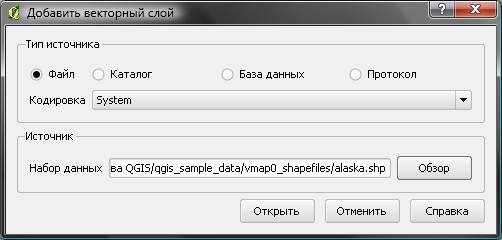
\includegraphics[clip=true, width=12cm]{addvectorlayerdialog}
   \caption{Ajouter une couche vecteur \nixcaption}\label{fig:addvectorlayer}
\end{center} 
\end{figure}

\begin{figure}[ht]
  \begin{center} 
  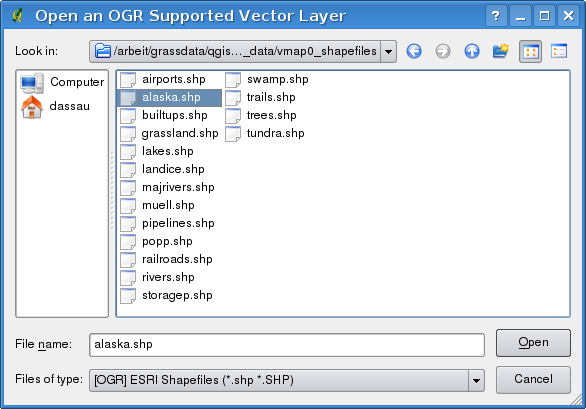
\includegraphics[clip=true, width=12cm]{shapefileopendialog}
  \caption{Fenêtre pour ouvrir une couche vecteur gérée par OGR \nixcaption}\label{fig:openshapefile}
\end{center}
\end{figure}

\begin{figure}[ht]
  \begin{center}
  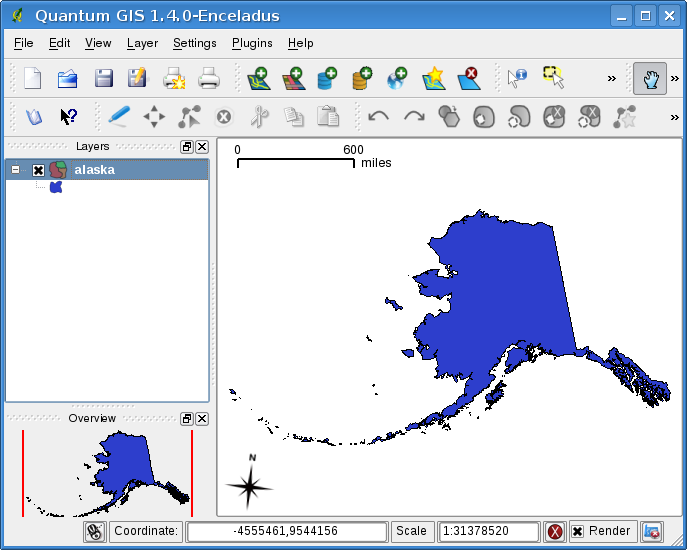
\includegraphics[clip=true, width=12cm]{shapefileloaded}
    \caption{\qg avec le Shapefile de l'Alaska chargé \nixcaption}\label{fig:loadedshapefile}
\end{center}
\end{figure}

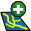
\includegraphics[width=0.7cm]{mActionAddNonDbLayer} Pour charger un shapefile, lancer \qg et cliquez sur \toolbtntwo{mActionAddNonDbLayer}{Ajouter une couche vecteur} dans la barre d'outil\index{shapefile!chargement} ou taper simplement \keystroke{V}. Ce même outil peut être utilisé pour charger tous les formats gérés par la bibliothèque OGR.
\par
L'outil ouvre alors une fenêtre de dialogue standard (voir Figure \ref{fig:openshapefile}) qui vous permet de naviguer dans les répertoires et les fichiers et charger le shapefile ou tout autre format géré.
La boîte de sélection \selectstring{Fichiers de type \dots} vous permet de présélectionner un format de fichier géré par OGR.
\par
Si vous le souhaitez, vous pouvez également sélectionner le type de codage du shapefile.
\par
Sélectionner un shapefile dans la liste puis cliquer sur \button{Ouvrir} le charge dans \qg. La figure \ref{fig:loadedshapefile} montre \qg après avoir chargé le fichier \filename{alaska.shp}.

%\begin{Tip}\caption{\textsc{Layer Colors}}
\begin{Tip}\caption{\textsc{Couleurs de couches}}
%\qgistip{When you add a layer to the map, it is assigned a random color. When adding more than one layer at a time, different colors are assigned to each layer.}
Quand vous ajoutez une couche sur une carte, une couleur aléatoire lui est assignée. En ajoutant plusieurs couches en une fois, différentes couleurs sont assignées à chacune des couches.
\end{Tip}

%Once loaded, you can zoom around the shapefile using the map navigation tools.
%To change the symbology of a layer, open the \dialog{Layer Properties} dialog by double clicking on the layer name or by right-clicking on the name in the legend and choosing \dropmenuopt{Properties} from the popup menu. See Section \ref{sec:symbology} for more information on setting symbology of vector layers.
Une fois chargée, vous pouvez zoomer sur le shapefile en utilisant les outils de navigation sur la carte.
Pour changer la symbologie d'une couche, ouvrez la fenêtre \dialog{Propriétés de la Couche} en double-cliquant sur le nom de la couche ou en faisant un clic droit sur son nom dans la légende et en choisissant \dropmenuopt{Propriétés} dans le menu qui apparait. Pour plus de détails sur les paramètres de la symbologie des couches vectorielles, référez-vous à la Section \ref{sec:symbology}.

\begin{Tip}\caption{\textsc{Charger une couche et un projet depuis un lecteur externe sous \mac}}
Sous \mac, les lecteurs portables qui sont montés à ôté du disque dur primaire n'apparaissent pas dans Fichier -> Ouvrir un Projet comme attendu. Nous travaillons sur le support des fenêtres d'ouverture/enregistrement natifs d'OS X pour résoudre ce problème. Pour y pallier, vous pouvez taper \og /Volumes\fg dans la boîte de nom Fichier et appuyer sur Entrée. Vous pouvez ensuite parcourir les lecteurs externes et les montages réseaux.
\end{Tip}

%\subsection{Improving Performance}
\subsection{Améliorer les performances}

%To improve the performance of drawing a shapefile, you can create a spatial index. A \index{spatial index!shapefiles} spatial index will improve the  speed of both zooming and panning. Spatial indexes used by \qg have a \filename{.qix} extension.
Pour améliorer les performances de dessin d'un shapefile, vous pouvez créer un index spatial. Un \index{index spatial!shapefiles} index spatial améliorera à la fois la vitesse d'exécution du zoom et du déplacement panoramique. Les index spatiaux utilisés par \qg ont une extension \filename{.qix}.

%Use these steps to create the index:
Voici les étapes de création d'un index spatial :

\begin{itemize}[label=--]
%\item Load a shapefile.
\item Chargez un shapefile
%\item Open the \dialog{Layer Properties} dialog by double-clicking on the shapefile name in the legend or by right-clicking and choosing \dropmenuopt{Properties} from the popup menu.
\item Ouvrez la fenêtre \dialog{Propriétés de la Couche} en double-cliquant sur le nom de la couche dans la légende ou en faisant un clic droit et en choisissant \dropmenuopt{Propriétés} dans le menu qui apparait.
%\item In the tab \tab{General} click the \button{Create Spatial Index} button.
\item Dans l'onglet \tab{Général}, cliquez sur le bouton \button{Créez un index spatial}.
\end{itemize}

%\subsection{Loading a \map Layer}
%\index{vector layers!MapInfo}
\subsection{Charger une couche MapInfo}
\index{couches vecteur!MapInfo}

%To load a \map layer, click on the \toolbtntwo{mActionAddNonDbLayer}{Add a vector layer} toolbar bar button or type \keystroke{V}, change the file type filter to \selectstring{Files of Type}{[OGR] \map (*.mif *.tab *.MIF *.TAB)} and select the layer you want to load.
Pour charger une couche MapInfo, cliquez sur \toolbtntwo{mActionAddNonDbLayer}{Ajouter une couche vecteur} dans la barre d'outils ou tapez \keystroke{V}, changez le type de filtre pour\\ \selectstring{Fichiers de type [OGR] \map (*.mif *.tab *.MIF *.TAB)} et sélectionnez la couche que vous souhaitez charger.

%\subsection{Loading an ArcInfo Coverage}
%\index{vector layers!ArcInfo Coverage}
\subsection{Charger une couverture ArcInfo binaire}
\index{couches vecteur!couverture ArcInfo binaire}
Pour charger une couverture binaire ArcInfo, il faut cliquer sur le bouton\\ \toolbtntwo{mActionAddNonDbLayer}{Ajouter une couche vecteur} ou taper \keystroke{V} pour ouvrir le dialogue correspondant. Sélectionner le \radiobuttonon{Directory} et \selectstring {Type}{Arc/Ingo Binary Coverage}. Naviguez jusqu'au dossier contenant vos fichiers puis choisissez-les.
\par
De manière similaire vous pouvez directement charger les fichiers vecteurs UK National Transfer Format ainsi que le format TIGER brut de l'US Census Bureau.

%\section{PostGIS Layers}
\section{Couches PostGIS}
%\index{vector layers!PostGIS|see{PostGIS}}
\index{couches vecteur!PostGIS|voir{PostGIS}}
%\index{PostGIS!layers}
\index{PostGIS!couches}
\label{label_postgis}

%PostGIS layers are stored in a \psq database. The advantages of \pg are the spatial indexing, filtering and query capabilities it provides. Using PostGIS, vector functions such as select and identify work more accurately than with OGR layers in \qg.
Les couches \pg sont stockées dans une base de données PostgreSQL. Les avantages de \pg sont les possibilités d'indexation spatiale, de filtre et de requête qu'il fournit. En utilisant PostGIS, les fonctions vecteur telles que la sélection ou l'identification fonctionnent avec plus d'exactitude qu'avec les couches OGR dans \qg.

%To use \pg layers you must:\index{PostgreSQL!loading layers}
Pour charger une couche PostGIS, vous devez :\index{PostgreSQL!charger des couches}

\begin{itemize}[label=--]
%\item Create a stored connection in \qg to the \psq database (if one is not already defined).\index{PostgreSQL!connection}
\item Dans \qg, créez une connexion enregistrée à une base de données \psq (si elle n'a pas été encore définie).\index{PostgreSQL!connexion}
%\item Connect to the database.
\item Connectez-vous à la base de données.
%\item Select the layer to add to the map.
\item Sélectionnez la couche à ajouter à la carte.
%\item Optionally provide a SQL \usertext{where} clause to define which features to load from the layer.
\item En option vous pouvez fournir une clause SQL \usertext{where} pour définir les entités de la couche à charger.
%\item Load the layer.
\item Charger la couche.
\end{itemize}

%\subsection{Creating a stored Connection}\index{PostgreSQL!connection}\label{sec:postgis_stored}
\subsection{Créer une connexion enregistrée} \index{PostgreSQL!connexion} \label{sec:postgis_stored}

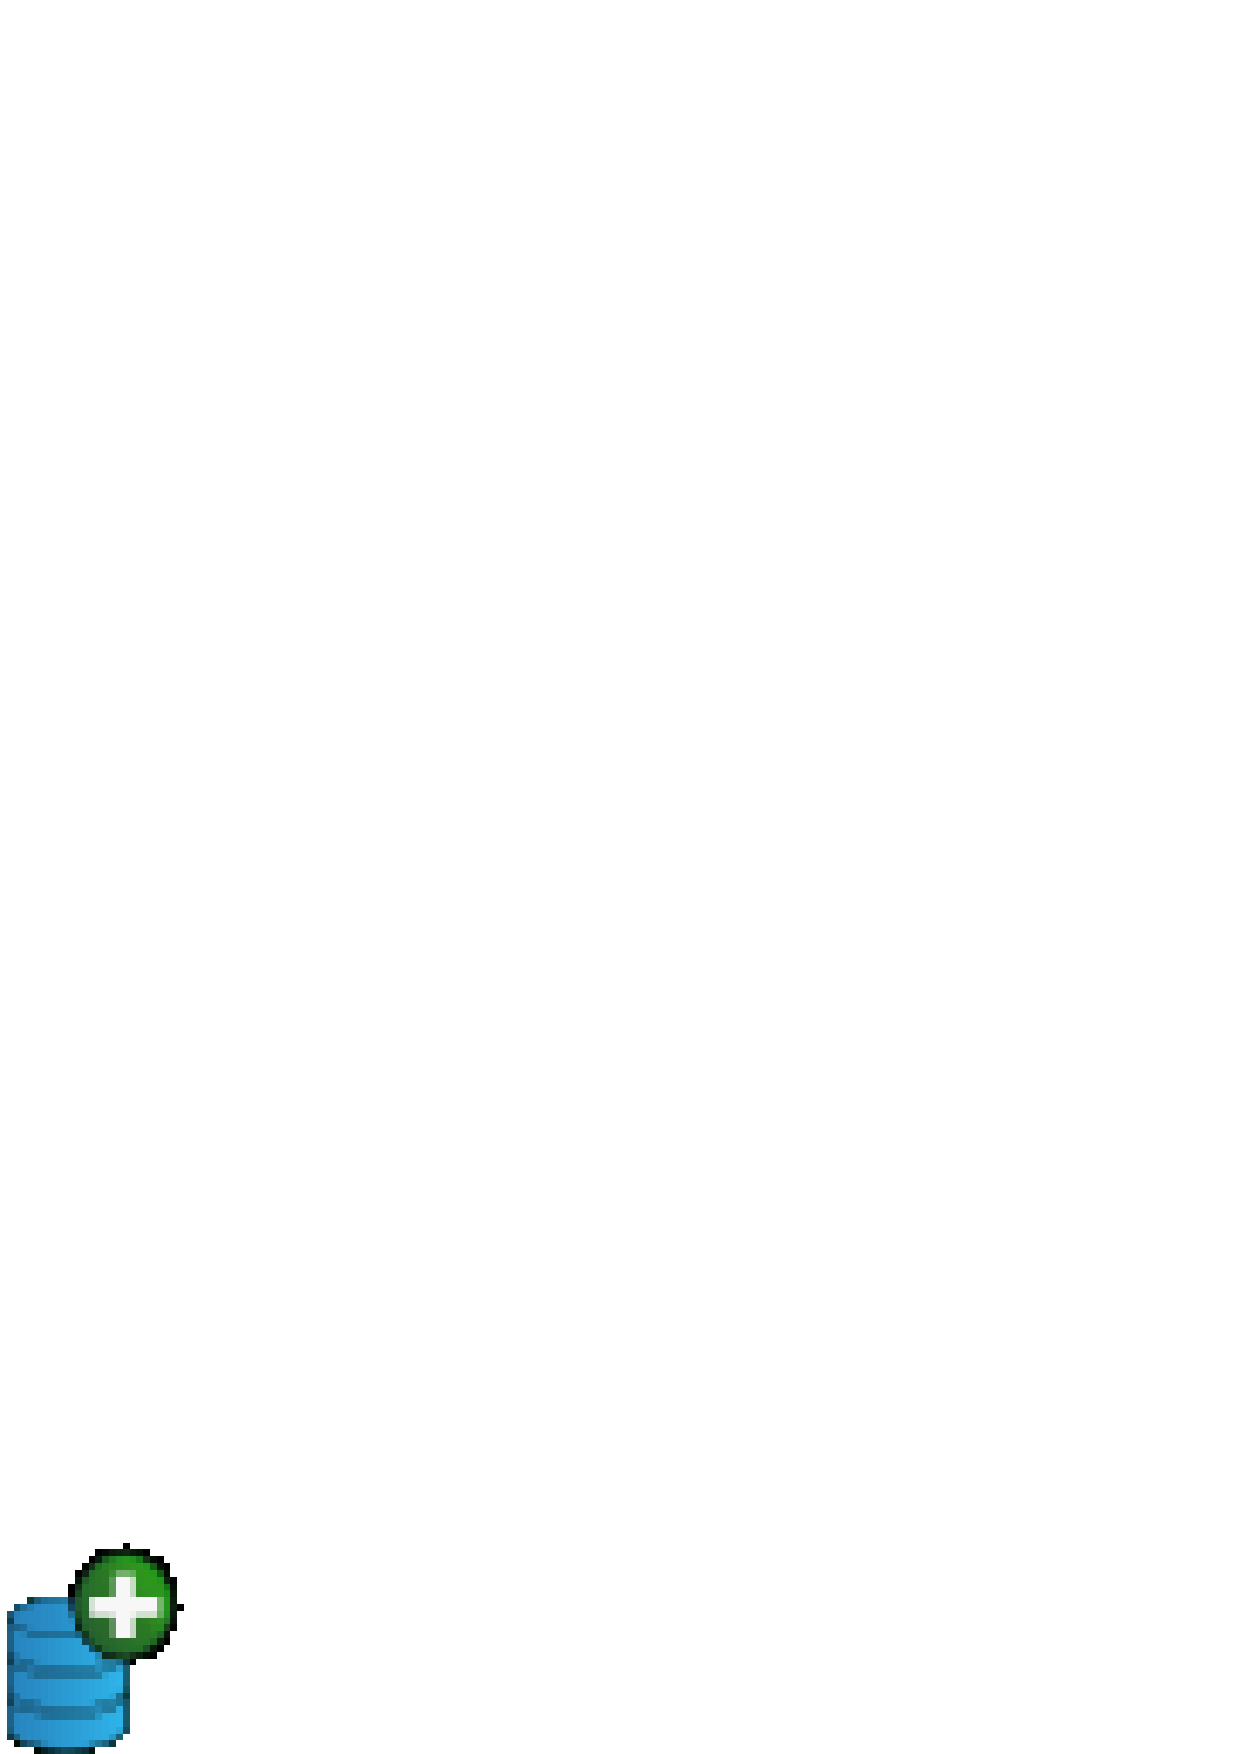
\includegraphics[width=0.7cm]{mActionAddLayer}
%The first time you use a \pg data source, you must create a connection to the \psq database that contains the data. Begin by clicking on the \toolbtntwo{mActionAddLayer}{Add a \pg Layer} toolbar button, selecting the \dropmenuopttwo{mActionAddLayer}{Add a \pg Layer...} option from the \mainmenuopt{Layer} menu or typing \keystroke{D}.
La première fois que utilisez une source de données PostGIS, vous devez créer une connexion à une base de données \psq qui contient les données. Commencez par cliquer sur le bouton \toolbtntwo{mActionAddLayer}{Ajouter une couche \pg} de la barre d'outils ou sélectionner l'option \dropmenuopttwo{mActionAddLayer}{Ajouter une couche PostGIS\dots} dans le menu \mainmenuopt{Couche} ou taper \keystroke{D}. Vous pouvez aussi ouvrir le dialogue \dialog{Ajouter une couche vecteur} et sélectionnez \radiobuttonon{Base de données}.
%The \dialog{Add \pg Table(s)} dialog will be displayed. To access the connection manager\index{PostgreSQL!connection manager}, click on the \button{New} button to display the \dialog{Create a New \pg Connection} dialog. The parameters required for a connection are shown in table \ref{tab:postgis_connection_parms}.
La fenêtre \dialog{Ajouter une ou plusieurs tables PostGIS} apparaît. Pour accéder au gestionnaire de connexion\index{PostgreSQL!gestionnaire de connexion}, cliquez sur le bouton \button{Nouveau} pour faire apparaitre la fenêtre\\ \dialog{Créer une nouvelle connexion PostGIS}. Les paramètres requis pour la connexion sont présentés dans le tableau \ref{tab:postgis_connection_parms}.

\begin{table}[ht]\index{PostgreSQL!connection parameters}
\centering
%\caption{PostGIS Connection Parameters}\label{tab:postgis_connection_parms}\medskip

\begin{tabular}{|l|p{11cm}|}
%\hline Name & A name for this connection. Can be the same as \textsl{Database}.\\
\hline Nom & Un nom pour cette connexion. Il peut être identique à \textsl{Base de données}.\\
%\hline Host \index{PostgreSQL!host} & Name of the database host. This must be a resolvable host name the same as would be used to open a telnet connection or ping the host. If the database is on the same computer as \qg, simply enter 'localhost' here.\\
\hline Hôte \index{PostgreSQL!host} & Nom pour l'hôte de la base de données. Il doit s'agir d'un nom existant, car il sera utilisé pour ouvrir une connexion Telnet ou interroger l'hôte. Si la base de données est sur le même ordinateur que \qg, mettez simplement \og localhost\fg. \\
%\hline Database \index{PostgreSQL!database} & Name of the database.\\
\hline Base de données \index{PostgreSQL!database} & Nom de la base de données.\\
%\hline Port \index{PostgreSQL!port}& Port number the \psq database server listens on. The default port is 5432.\\
\hline Port \index{PostgreSQL!port}& Numéro de port que le serveur de base de données \psq écoute. Le port par défaut est 5432.\\
%\hline Username \index{PostgreSQL!username}& User name used to login to the database.\\
\hline Nom d'utilisateur \index{PostgreSQL!username} & Nom d'utilisateur utilisé pour se connecter à la base de données.\\
%\hline Password \index{PostgreSQL!password}& Password used with \textsl{Username} to connect to the database.\\
\hline Mot de passe \index{PostgreSQL!password} & Mot de passe utilisé avec le \textsl{Nom d'utilisateur} pour se connecter à la base de données.\\
%\hline SSL mode \index{PostgreSQL!sslmode}& How the SSL connection will be negotiated with the server. These are the options: 
\hline Mode SSL \index{PostgreSQL!sslmode} & Comment sera négociée la connexion SSL avec le serveur. Voici les options :
\begin {itemize}[label=--]
%\item disable: only try an unencrypted SSL connection;
\item désactiver : essayer une connexion SSL non cryptée uniquement
%\item allow: try a non-SSL connection, if that fails, try an SSL connection;
\item permettre : essayer une connexion non-SSL. Si cela échoue, essayer une connexion SSL;
%\item prefer (the default): try an SSL connection, if that fails, try a non-SSL connection;
\item préferer (par défaut): essayer une connexion SSL. Si cela échoue une connexion non-SSL;
\item requiert: essayer seulement une connexion SSL
\end {itemize}
Il faut noter qu'une accélération massive du rendu des couches \pg peut être obtenue en désactivant le SSL dans l'éditeur de connexion. \\
\hline
\end{tabular}
\caption{Paramètres de connexion PostGIS}\label{tab:postgis_connection_parms}
\end{table}

%Optional you can activate follwing checkboxes:
Vous pouvez également activer les options suivantes :

\begin{itemize}[label=--]
%\item \checkbox{Save Password}
\item \checkbox{Sauvegarder le mot de passe}
%\item \checkbox{Only look in the geometry\_columns table}
\item \checkbox{Uniquement regarder la table geometry\_columns}
%\item \checkbox{Only look in the 'public' schema}
\item \checkbox{Uniquement regarder dans le schéma 'public'}
\end{itemize}

%Once all parameters and options are set, you can test the connection by clicking on the \button{Test Connect} button\index{PostgreSQL!connection!testing}.
Une fois que tous les paramètres et les options sont définis, vous pouvez tester la connexion en cliquant que le bouton  \button{Test de connexion}\index{PostgreSQL!connexion!test}.

%\begin{Tip}\caption{\textsc{\qg User Settings and Security}}\index{settings}\index{security}
\begin{Tip}\caption{\textsc{Paramètres utilisateur de \qg et Sécurité}}\index{paramètres}\index{sécurité}
%\qgistip{Your customized settings for \qg are stored based on the operating system. \nix, the settings are stored in your home directory in \filename{.qt/qgisrc}. \win, the settings are stored in the registry. Depending on your computing environment, storing passwords in your \qg settings may be a security risk.}
Vos paramètres personnalisés pour \qg sont stockés différemment selon le système d'exploitation. \nix, les paramètres sont stockés dans votre répertoire home dans \filename{.qt/qgisrc}. \win, les paramètres sont stockés dans la base de registre. Selon votre environnement informatique, stocker vos mots de passe dans vos paramètres \qg peut présenter des risques vis-à-vis de la sécurité.
\end{Tip}

%\subsection{Loading a \pg Layer}\index{PostgreSQL!loading layers}
\subsection{Charger une couche PostGIS}\index{PostgreSQL!charger des couches}

%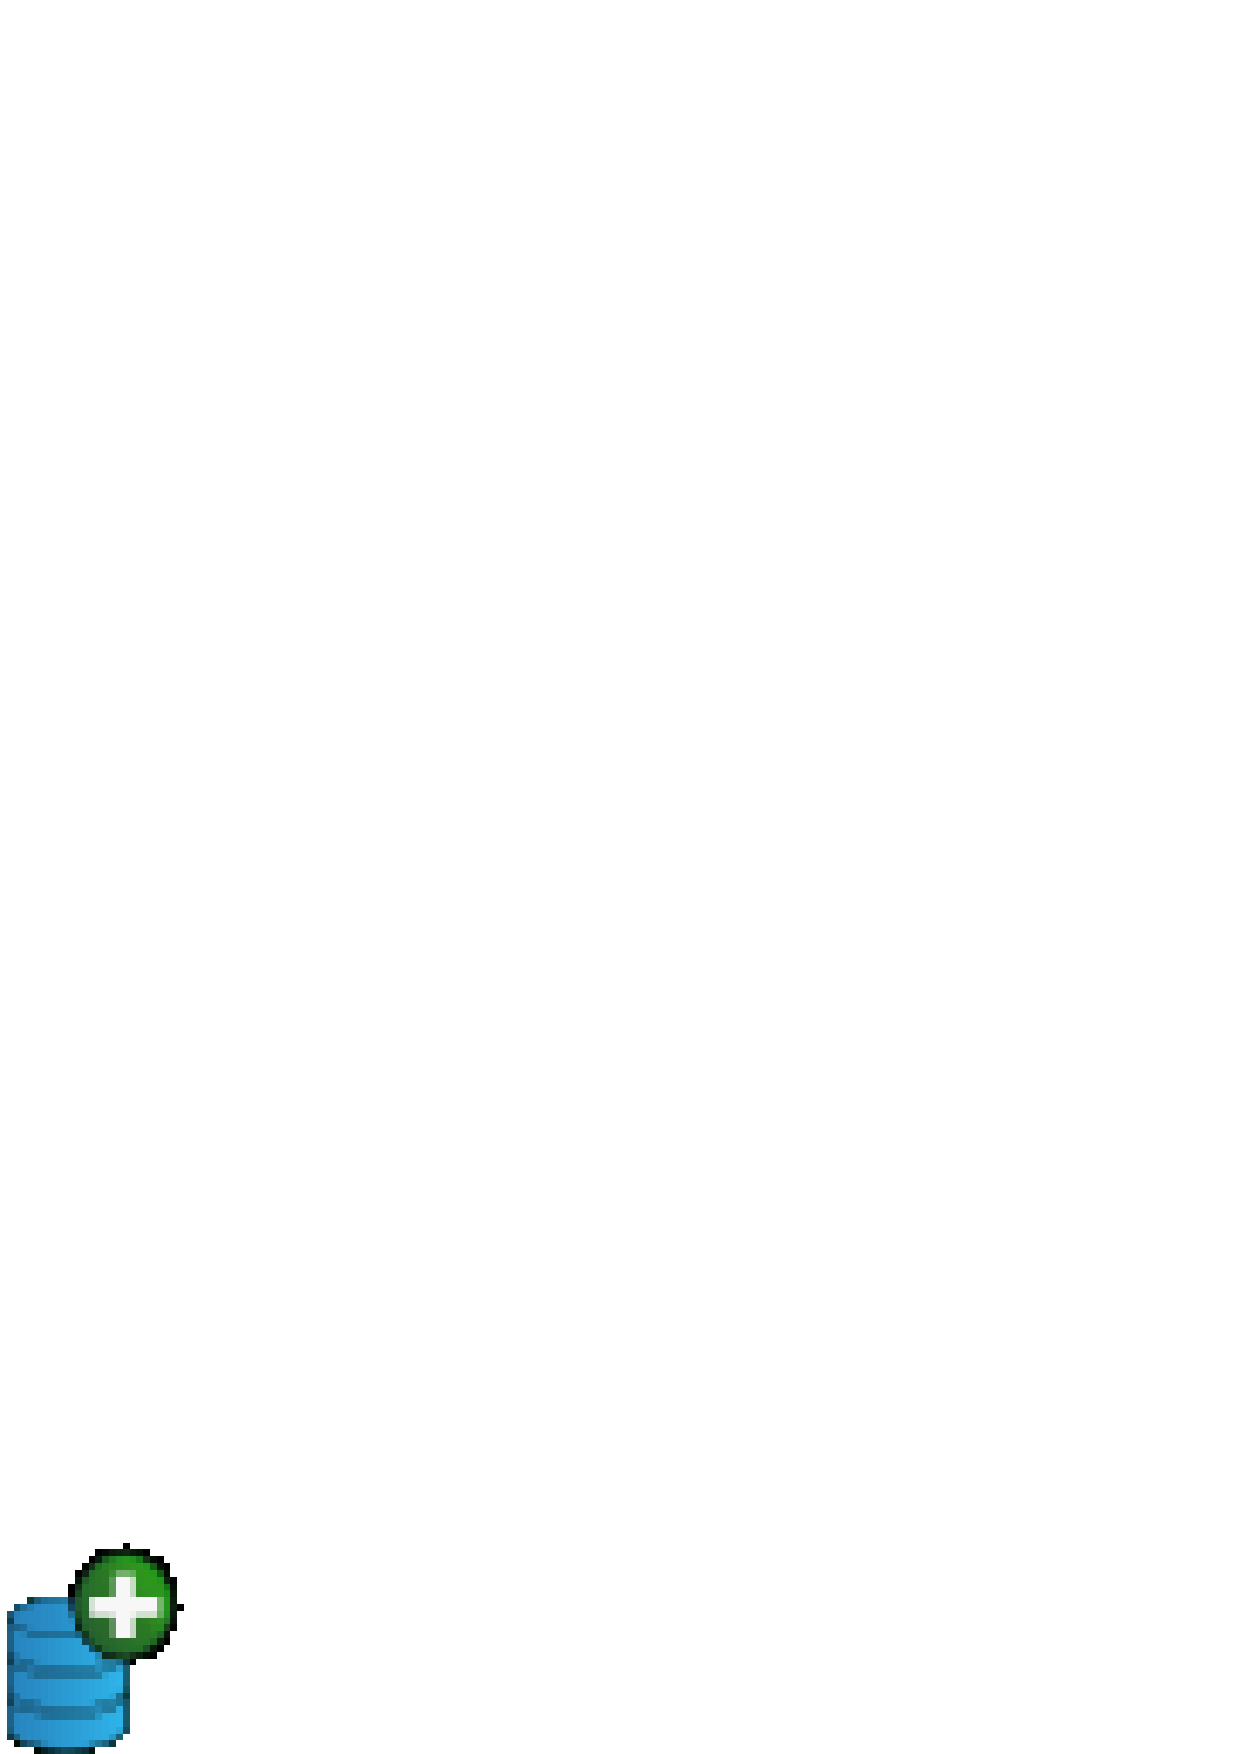
\includegraphics[width=0.7cm]{mActionAddLayer} Once you have one or more connections defined, you can load layers from the \psq database. Of course this requires having data in PostgreSQL. See Section \ref{sec:loading_postgis_data} for a discussion on importing data into the database.
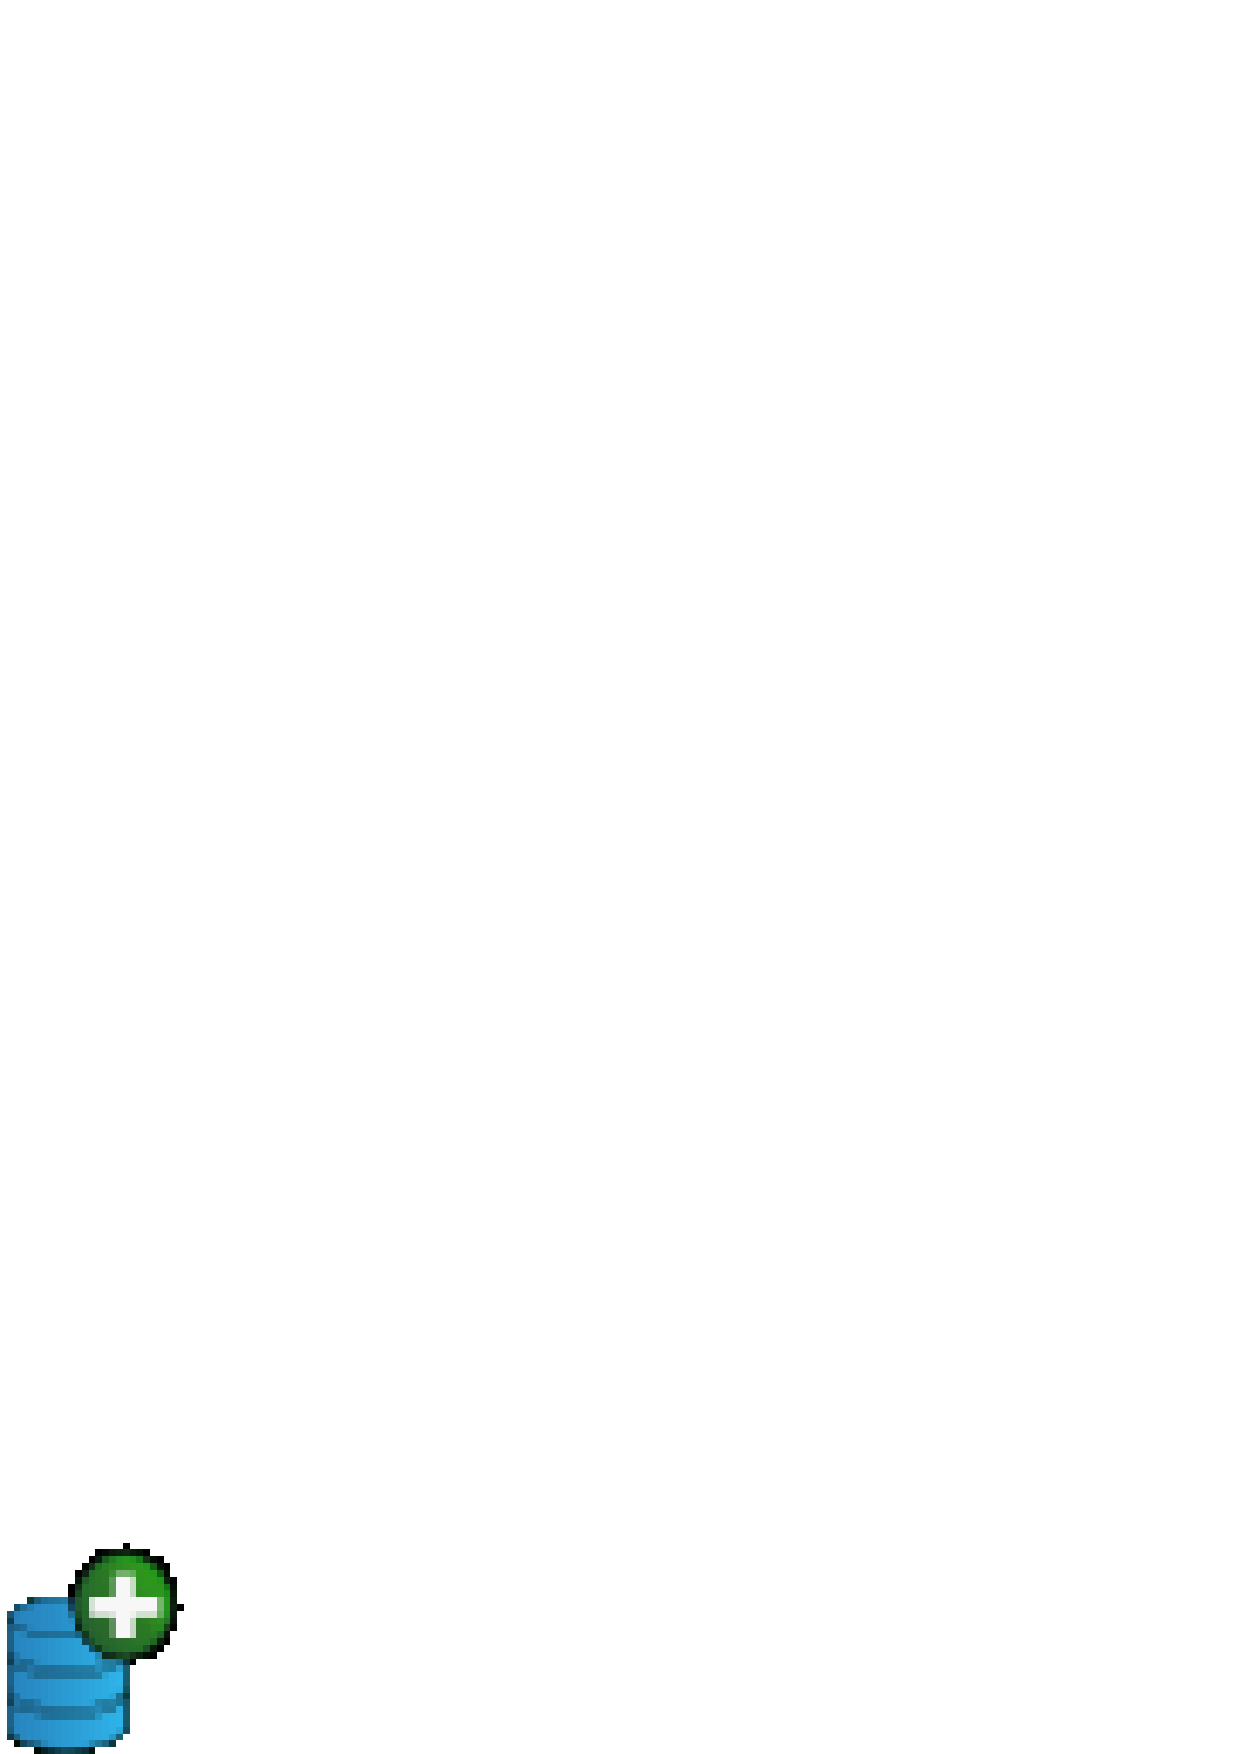
\includegraphics[width=0.7cm]{mActionAddLayer} Une fois une ou plusieurs connexions définies, vous pouvez charger des couches de la base de données PostgreSQL. Bien sûr, cela nécessite d'avoir des données dans PostgreSQL. Référez-vous à la Section \ref{sec:loading_postgis_data} pour plus de détails concernant l'importation de données dans la base de données.

%To load a layer from PostGIS, perform the following steps:
Pour charger une couche PostGIS, suivez ces étapes :

\begin{itemize}[label=--]
%\item If the \dialog{Add \pg Table(s)} dialog is not already open, click on the \toolbtntwo{mActionAddLayer}{Add a \pg Layer} toolbar button.
\item Si la fenêtre \dialog{Ajouter une ou plusieurs tables PostGIS} n'est pas ouverte, cliquez sur le bouton \toolbtntwo{mActionAddLayer}{Ajouter une couche PostGIS} de la barre d'outils.
%\item Choose the connection from the drop-down list and click \button{Connect}.
\item Choisissez la connexion dans la liste déroulante et cliquez sur \button{Connecter}.
%\item Find the layer you wish to add in the list of available layers.
\item Trouvez la couche que vous souhaitez ajouter dans la liste des couches disponibles.
%\item Select it by clicking on it. You can select multiple layers by holding down the \keystroke{shift} key while clicking. See Section \ref{sec:query_builder} for information on using the \psq Query Builder to further define the layer.
\item Sélectionnez la en cliquant dessus. Vous pouvez sélectionner plusieurs couches en gradant la touche \keystroke{shift} enfoncée quand vous cliquez. Référez-vous à la Section \ref{sec:query_builder} pour plus d'informations sur l'utilisation du Constructeur de requête de \psq pour mieux définir la couche.
%\item Click on the \button{Add} button to add the layer to the map.
\item Cliquez sur le bouton \button{Ajouter} pour ajouter la couche à la carte.
\end{itemize}

%\begin{Tip}\caption{\textsc{PostGIS Layers}}
\begin{Tip}\caption{\textsc{Couches PostGIS}}
%\qgistip{Normally a \pg layer is defined by an entry in the geometry\_columns table. From version \OLD % should be 0.9.0 on, \qg can load layers that do not have an entry in the geometry\_columns table. This includes both tables and views. Defining a spatial view provides a powerful means to visualize your data. Refer to your \psq manual for information on creating views.}
Normalement, une couche \pg est définie par une entrée dans la table geometry\_columns. Depuis la version 0.11.0, \qg peut charger des couches qui n'ont pas d'entrée dans la table geometry\_columns. Ceci concerne aussi bien les tables que les vues. Définir une vue spatiale fournit un moyen puissant pour visualiser vos données. Référez-vous à votre manuel \psq pour plus d'informations sur la création des vues.
\end{Tip}

%\subsection{Some details about \psq layers}\label{sec:postgis_details}
%\index{PostgreSQL!layer details}
\subsection{Quelques éléments de détail à propos des couches PostgreSQL} \label{sec:postgis_details}
\index{PostgreSQL!détails sur les couches}

%This section contains some details on how \qg accesses \psq layers. Most of the time \qg should simply provide you with a list of database tables that can be loaded, and load them on request. However, if you have trouble loading a \psq table into \qg, the information below may help you understand any \qg messages and give you direction on changing the \psq table or view definition to allow \qg to load it.
Cette section contient quelques détails sur la manière dont \qg accède aux couches PostgreSQL. La plupart du temps, \qg devrait simplement fournir une liste de tables de base de données qui peuvent être chargées et les charge à la demande. Cependant, si vous avez des problèmes pour charger une table \psq dans \qg, les informations données ci-dessous peuvent vous aider à comprendre les messages de \qg et vous donnez une indication sur comment changer la table ou la vue \psq pour qu'elle se charge dans \qg.

%\qg requires that \psq layers contain a column that can be used as a unique key for the layer. For tables this usually means that the table needs a primary key, or a column with a unique constraint on it. \qg additionally requires that this column be of type int4 (an integer of size 4 bytes). If a table lacks these items, the oid column will be used instead. Performance will be improved if the column is indexed (note that primary keys are automatically indexed in PostgreSQL).
\qg demande que les couches \psq aient un champ qui peut être utilisé comme clé unique pour la couche. Pour les tables, cela signifie qu'elles doivent avoir une clé primaire ou un champ ayant une contrainte d'unicité. De plus, \qg impose que cette colonne soit de type int4 (un entier de 4 bites). Alternativement la colonne ctid peut être utilisée comme clé primaire. Si une table ne respecte pas ces conditions, le champ oid sera utilisé à la place. Les performances seront améliorées si le champ est indexé (notez que les clés primaires sont automatiquement indexées dans PostgreSQL).

%If the \psq layer is a view, the same requirements exists, but views don't have primary keys or columns with unique constraints on them. In this case \qg will try to find a column in the view that is derived from a table column that is suitable. If one cannot be found, \qg will not load the layer. If this occurs, the solution is to alter the view so that it does include a suitable column (a type of int4 and either a primary key or with a unique constraint, preferably indexed).
Si la couche \psq est une vue, les mêmes conditions s'appliquent, mais elles n'ont pas de clé primaire ou de champ ayant une contrainte d'unicité. Dans ce cas, \qg essayera de trouver un champ de la vue issu d'un champ une table qui convienne en parcourant la définition SQL de la vue. Cependant, il y a certains aspects du SQL que \qg ignore tel que l'utilisation d'alias ou de colonnes générées par des fonctions. S'il ne peut pas en trouver, \qg ne chargera pas la couche. Si cela arrive, la solution consiste à modifier la vue de telle sorte qu'elle inclut un champ qui convienne (de type int4 et ayant soit une clé primaire soit une contrainte d'unicité, de préférence indexée).

%\subsection{Importing Data into PostgreSQL}\label{sec:loading_postgis_data}\index{PostGIS!SPIT!importing data}
\subsection{Importer des données dans PostgreSQL} \label{sec:loading_postgis_data}\index{PostGIS!SPIT!importer des données}

\minisec{shp2pgsql}
%Data can be imported into \psq using a number of methods. \pg includes a utility called \filename{shp2pgsql} that can be used to import shapefiles into a \pg enabled database. For example, to import a shapefile named \filename{lakes.shp} into a \psq database named \usertext{gis\_data}, use the following command:
De multiples méthodes existent pour importer des données dans PostgreSQL. \pg incluent un utilitaire nommé \filename{shp2pgsql} qui peut être utilisé pour importer des shapefiles dans des bases de données disposant de PostGIS. Par exemple, pour importer le shapefile \filename{lakes.shp} dans une base de données \psq nommée \usertext{gis\_data}, utiliser la commande suivante :

\begin{verbatim}
  shp2pgsql -s 2964 lakes.shp lakes_new | psql gis_data
\end{verbatim}

%This creates a new layer named \usertext{lakes\_new} in the \usertext{gis\_data} database. The new layer will have a spatial reference identifier (SRID) of 2964. See Section \ref{label_projections} for more information on spatial reference systems and projections.
Ceci crée une nouvelle couche nommée \usertext{lakes\_new} dans la base de données usertext{gis\_data}. La nouvelle couche aura l'identifiant de référence spatiale (SRID) 2964. Référez-vous à la Section \ref{label_projections} pour plus d'informations sur les systèmes de référence spatiale et les projections.
\begin{Tip}
%\caption{\textsc{Exporting datasets from PostGIS}\index{PostGIS!Exporting}}
\caption{\textsc{Exporter des jeux de données depuis PostGIS}\index{PostGIS!Exporter}}
%\qgistip{Like the import-tool \filename{shp2pgsql} there is also a tool to export PostGIS-datasets as shapefiles: \filename{pgsql2shp}. This is shipped within your \pg distribution.}
Comme l'outil d'importation \filename{shp2pgsql}, il y a également un outil d'exportation de jeux de données \pg en shapefile : \filename{pgsql2shp}. Cet outil est inclus dans la distribution de PostGIS.
\end{Tip}

%\minisec{SPIT Plugin}
\minisec{Extension SPIT}
%
\includegraphics[width=0.7cm]{spiticon} \qg comes with a plugin named SPIT (Shapefile to \pg Import Tool)\index{PostGIS!SPIT}. SPIT can be used to load multiple shapefiles at one time and includes support for schemas. To use SPIT, open the Plugin Manager from the \mainmenuopt{Plugins} menu, check the box next to the \checkbox{SPIT plugin} and click \button{OK}. The SPIT icon will be added to the plugin toolbar\index{PostGIS!SPIT!loading}.

\includegraphics[width=0.7cm]{spiticon.png} \qg est distribué avec une extension nommée SPIT (Shapefile to \pg Import Tool)\index{PostGIS!SPIT}. SPIT peut être utilisé pour charger plusieurs shapefiles en une fois et inclut la gestion des schémas. Pour utiliser SPIT, ouvrez le Gestionnaire d'extensions depuis le menu \mainmenuopt{Plugins}, cochez la case adjacente à \checkbox{SPIT plugin} et cliquez sur \button{OK}. L'icône SPIT sera ajoutée à la barre d'outils\index{PostGIS!SPIT!charger}.

%To import a shapefile, click on the \toolbtntwo{spiticon}{SPIT} tool in the toolbar to open the \dialog{SPIT - Shapefile to \pg Import Tool} dialog. Select the \pg database you want to connect to and click on \button{Connect}. Now you can add one or more files to the queue by clicking on the \button{Add} button. To process the files, click on the \button{OK} button. The progress of the import as well as any errors/warnings will be displayed as each shapefile is processed.
Pour importer un shapefile, cliquez sur le bouton \toolbtntwo{spiticon}{SPIT} dans la barre d'outils pour ouvrir la fenêtre \dialog{SPIT - Outil d'importation de Shapefile dans PostGIS}. Sélectionnez la base de données à laquelle vous voulez vous connecter et cliquez sur le bouton \button{Connecter}. Vous pouvez alors ajouter un ou plusieurs fichiers à la liste en cliquant sur le bouton \button{Ajouter}. Pour traiter les fichiers, appuyez sur le bouton \button{OK}. La progression de l'importation aussi bien que les erreurs ou les alertes s'afficheront pour chaque shapefile.

%\begin{Tip}\caption{\textsc{Importing Shapefiles Containing \psq Reserved Words}}\index{PostGIS!SPIT!reserved words}
\begin{Tip}\caption{\textsc{Importer des shapefiles contenant des mots réservés de PostgreSQL}}\index{PostGIS!SPIT!mots réservés}
%\qgistip{If a shapefile is added to the queue containing fields that are reserved words in the \psq database a dialog will popup showing the status of each field. You can edit the field names\index{PostGIS!SPIT!editing field names} prior to import and change any that are reserved words (or change any other field names as desired). Attempting to import a shapefile with reserved words as field names will likely fail.}
Si un shapefile est ajouté à la liste et que des noms de champs correspondent à des mots réservés dans une base de données PostgreSQL, une fenêtre apparaitra et montrera le statut de chaque champ. Vous pouvez éditer les noms des champs\index{PostGIS!SPIT!éditer des noms de champ} avant l'importation et changer ceux qui correspondent à un mot réservé (ou faire les changements désirés). Toute tentative d'importer un shapefile ayant un champ contenant un mot réservé devrait vraisemblablement échouer.
\end{Tip}

\minisec{ogr2ogr}
%Beside \filename{shp2pgsql} and \filename{SPIT} there is another tool for feeding geodata in PostGIS: \filename{ogr2ogr}. This is part of your GDAL installation.
En plus de \filename{shp2pgsql} et \filename{SPIT}, un autre outil est fourni pour importer des données géographiques dans \pg : \filename{ogr2ogr}. Il est inclus dans GDAL.
%To import a shapefile into PostGIS, do the following:
Pour importer un shapefile dans PostGIS, tapez la commande suivante :
\begin{verbatim}
  ogr2ogr -f "PostgreSQL" PG:"dbname=postgis host=myhost.de user=postgres \
  password=topsecret" alaska.shp
\end{verbatim}

%This will import the shapefile \filename{alaska.shp} into the PostGIS-database \usertext{postgis} using the user \usertext{postgres} with the password \usertext{topsecret} on host \server{myhost.de}.
Ceci va importer le shapefile \filename{alaska.shp} dans la base de données \pg \usertext{postgis} en utilisant l'utilisateur \usertext{postgres} avec le mot de passe \usertext{topsecret} sur l'hôte \server{myhost.de}.

%Note that OGR must be built with \psq to support PostGIS. You can see this by typing
Notez qu'OGR doit être compilé avec \psq pour gérer PostGIS. Vous pouvez vérifier en tapant :
\begin{verbatim}
ogrinfo --formats | grep -i post
\end{verbatim}

%If you like to use PostgreSQL's \filename{COPY}-command instead of the default \filename{INSERT INTO} method you can export the following environment-variable (at least available on \nix and \osx):
Si vous préférez utiliser la commande \psq \filename{COPY} au lieu de la méthode par défaut, \filename{INSERT INTO}, vous pouvez exporter la variable d'environnement suivante (au moins sur \nix et \osx) :
\begin{verbatim}
  export PG_USE_COPY=YES
\end{verbatim}

%\filename{ogr2ogr} does not create spatial indexes like \filename{shp2pgsl} does. You need to create them manually using the normal SQL-command \filename{CREATE INDEX} afterwards as an extra step (as described in the next section \ref{label_improve}).
\filename{ogr2ogr} ne crée pas d'index spatial comme le fait \filename{shp2pgsl}. Vous devez effectuer une étape supplémentaire et le créer manuellement après en utilisant la commande SQL classique \filename{CREATE INDEX} (comme cela est détaillé dans la section suivante \ref{label_improve}).

%\subsection{Improving Performance} \label{label_improve}
\subsection{Améliorer les performances} \label{label_improve}

%Retrieving features from a \psq database can be time consuming, especially over a network. You can improve the drawing performance of \psq layers by ensuring that a \index{PostGIS!spatial index} spatial index exists on each layer in the database. \pg supports creation of a \index{PostGIS!spatial index!GiST} GiST (Generalized Search Tree) index to speed up spatial searches of the data.
Récupérer des entités depuis une base de données \psq peut être long, surtout par un réseau. Vous pouvez améliorer les performances de dessin de couches \psq en vous assurant qu'un \index{PostGIS!index spatial} index spatial existe pour chaque couche dans la base de données. \pg gère la création d'un index \index{PostGIS!index spatial!GiST} GiST (Generalized Search Tree) pour accélérer les recherches spatiales sur les données.

%The syntax for creating a GiST\footnote{GiST index information is taken from the \pg documentation available at \url{http://postgis.refractions.net}} index is:
La syntaxe pour créer un index GiST\footnote{les informations de l'index GiST proviennent de la documentation de \pg disponible sur \url{http://postgis.refractions.net}} est la suivante :

\begin{verbatim}
    CREATE INDEX [indexname] ON [tablename]
      USING GIST ( [geometryfield] GIST_GEOMETRY_OPS );
\end{verbatim}

%Note that for large tables, creating the index can take a long time. Once the index is created, you should perform a \usertext{VACUUM ANALYZE}. See the \pg documentation \cite{PostGISweb} for more information.
Notez que pour de grandes tables, créer un index peut prendre du temps. Une fois cet index créé, vous devriez faire une \usertext{VACUUM ANALYZE}. Référez-vous à la documentation de \cite{PostGISweb} pour plus d'informations.

%The following is an example of creating a GiST index:
Voici un exemple de création d'un index GiST :
\begin{verbatim}
gsherman@madison:~/current$ psql gis_data
Welcome to psql 8.3.0, the \psq interactive terminal.

Type:  \copyright for distribution terms
        \h for help with SQL commands
        \? for help with psql commands
        \g or terminate with semicolon to execute query
        \q to quit

gis_data=# CREATE INDEX sidx_alaska_lakes ON alaska_lakes
gis_data-# USING GIST (the_geom GIST_GEOMETRY_OPS);
CREATE INDEX
gis_data=# VACUUM ANALYZE alaska_lakes;
VACUUM
gis_data=# \q
gsherman@madison:~/current$
\end{verbatim}

\subsection{Couches vecteurs dépassants les 180\degres{} de longitude}
\index{vector layers!crossing}

Beaucoup de logiciels de SIG ne traitent pas les cartes vecteurs  ayant un système de référence géographique dépassant la ligne des 180\degres{} de longitude. Il en résulte que sous \qg on verra 2 emplacements distincts et éloignés qui devraient être proches l'un de l'autre. Sur la figure \ref{fig:vector_not_wrapping} le petit point tout à gauche sur le canevas cartographique (Chatham Island) devrait être dans la grille, à droite des îles principales de Nouvelle-Zélande.

\begin{figure}[ht]
   \begin{center}
   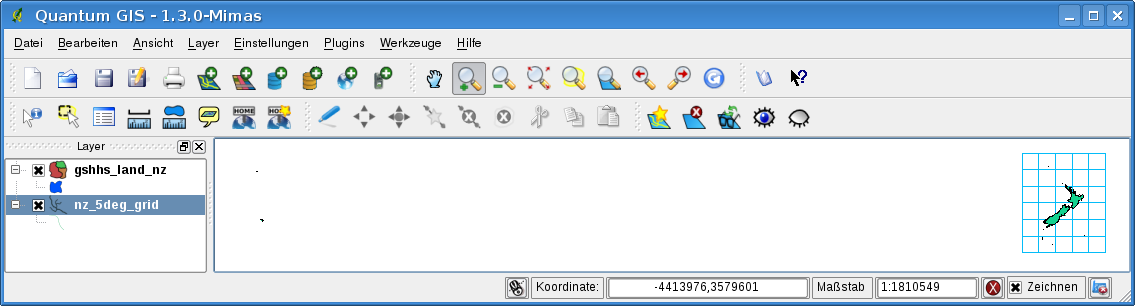
\includegraphics[clip=true, width=\textwidth]{vectorNotWrapping}
   \caption{Carte en lat/lon dépassant les 180\degres{} de longitude \nixcaption}
   \label{fig:vector_not_wrapping}
\end{center}
\end{figure}

Une solution est de transformer les valeurs longitudinales en utilisant \pg et la fonction \textbf{ST\textunderscore Shift\textunderscore Longitude}
\footnote{\url{http://postgis.refractions.net/documentation/manual-1.4/ST_Shift_Longitude.html}}. Cette fonction lit chaque point/sommet de chacune des entités dans une géométrie et si la coordonnée de longitude est inférieure à 0\degres{} elle lui ajoute 360\degres{}. Le résultat est une version de 0\degres{} -- 360\degres{} version des données sur une carte centré à 180\degres{}.

\begin{figure}[ht]
   \begin{center}
   
   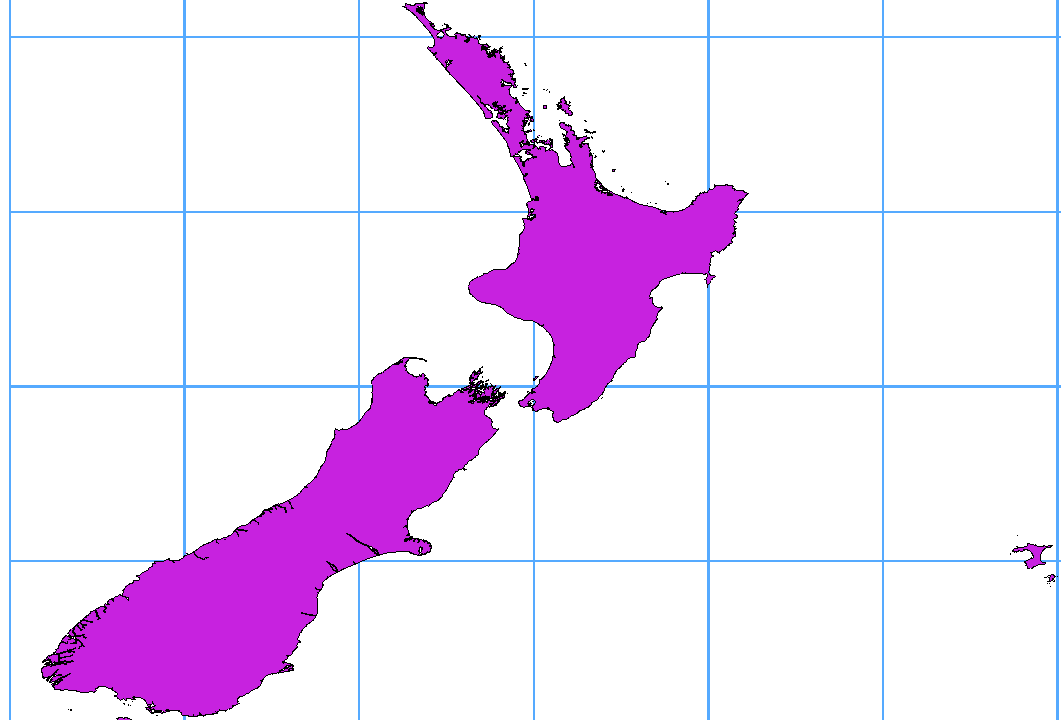
\includegraphics[clip=true, width=9cm]{vectorWrapping}
   \caption{Carte dépassant la ligne des 180\degres{} de longitude après application de la fonction ST\textunderscore Shift\textunderscore Longitude}
\label{fig:vector_wrapping}
\end{center}
\end{figure}

\minisec{Usage}

\begin{itemize}[label=--]
\item Importer des données vers \pg (\ref{sec:loading_postgis_data}) en utilisant par exemple l'extension de gestion de \pg (PostGIS Manager) ou l'extension SPIT
\item Utiliser l'interface en ligne de commande \pg pour exécuter la commande suivante (c'est un exemple où \og TABLE\fg est bien le nom de votre table PostGIS) \\ 
\texttt{gis\_data=\# update TABLE set the\_geom=ST\_shift\_longitude(the\_geom);} 
\item Si tout ce passe bien, vous devriez recevoir une confirmation sur le nombre d'entités qui ont été mise à jour, puis vous pouvez charger la carte et voir la différence (Figure \ref{fig:vector_wrapping})
\end{itemize}

\section{Couches SpatiaLite} 
\index{SpatiaLite layers!properties dialog}
\index{vector layers!SpatlaLIte|see{SpatiaLite}}
\index{SpatiaLite!layers}
\label{label_spatialite} 

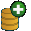
\includegraphics[width=0.7cm]{mActionAddSpatiaLiteLayer}
La première fois que vous chargerez une base Spatialite, commencez par cliquer sur le bouton \toolbtntwo{mActionAddSpatiaLiteLayer}{Ajouter une couche SpatiaLite} ou en sélectionnant l'option\\ \dropmenuopttwo{mActionAddSpatiaLiteLayer}{Ajouter une couche SpatiaLite\dots} depuis le menu \mainmenuopt{Couche} ou en tapant \keystroke{L}. Ceci fait apparaitre une fenêtre qui vous permet soit de vous connecter à une base déjà connue de \qg, que vous pouvez choisir dans une liste déroulante, ou définissant une nouvelle connexion. Pour ce faire, cliquez sur \button{Nouveau} et utilisez le navigateur de fichier pour pointer votre base SpatiaLite qui se termine par une extension \filename{.sqlite }.

%\section{The Vector Properties Dialog}\label{sec:vectorprops}
%\index{vector layers!properties dialog}
\section{La fenêtre Propriété des couches vecteur}\label{sec:vectorprops}
\index{couches vecteur!fenêtre propriété}

%The \dialog{Layer Properties} dialog for a vector layer provides information about the layer, symbology settings and labeling options. If your vector layer has been loaded from a \psq / \pg datastore, you can also alter the underlying SQL for the layer - either by hand editing the SQL on the \tab{General} tab or by invoking the \dialog{Query Builder} dialog on the \tab{General} tab. To access the \dialog{Layer Properties} dialog, double-click on a layer in the legend or right-click on the layer and select \dropmenuopt{Properties} from the popup menu.
La fenêtre \dialog{Propriétés de la couche} pour une couche vecteur fournit des informations sur la couche, les paramètres de représentation et les options d'étiquetage. Si votre couche a été chargée depuis une base \ppg, vous pouvez également modifier la requête SQL d'appel de la couche, soit manuellement en éditant le SQL dans l'onglet \tab{Général} soit en appelant la fenêtre \dialog{Constructeur de requête} depuis l'onglet \tab{Général}. Pour accéder à la fenêtre \dialog{Propriétés de la couche}, double-cliquez sur la couche dans la légende ou faites un clic droit sur la couche et sélectionnez \dropmenuopt{Propriétés} dans le menu qui apparait.

\begin{figure}[ht]
  \begin{center}
  %\caption{Vector Layer Properties Dialog \nixcaption}\label{fig:vector_symbology}\smallskip
  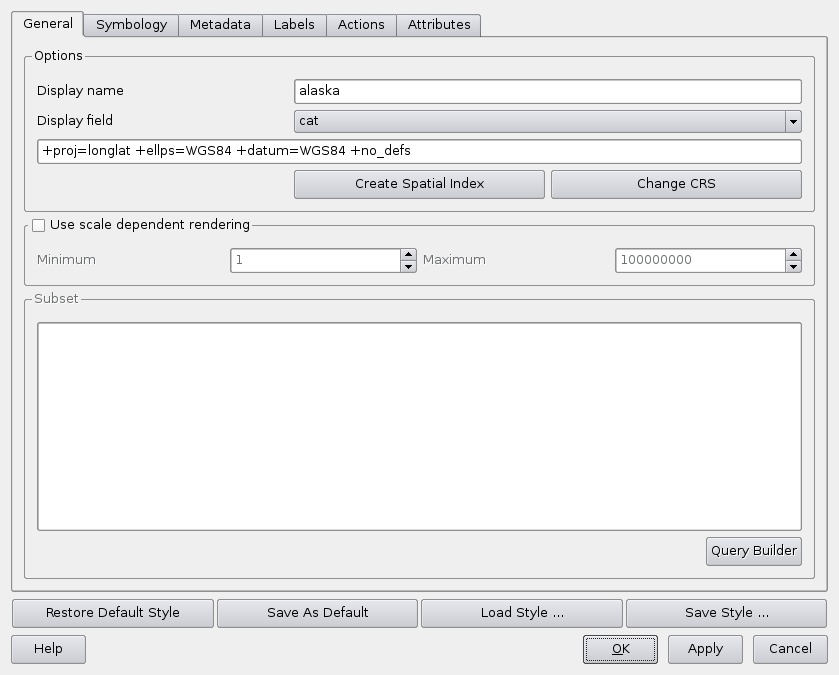
\includegraphics[clip=true, width=12cm]{vectorLayerSymbology}
  \caption{Fenêtre Propriétés d'une couche vecteur \nixcaption}\label{fig:vector_symbology}
\end{center}
\end{figure}

%\subsection{General Tab}\label{vectorgeneraltab}
\subsection{Onglet Général}\label{vectorgeneraltab}
%The \tab{General} tab is essentially like that of the raster dialog. It allows you to change the display name, set scale dependent rendering options, create a spatial index of the vector file (only for OGR supported formats and PostGIS) and view or change the projection of the specific vetor layer.
L'onglet \tab{Général} des couches vecteur est très proche de celui des couches raster. Il vous permet de changer le nom affiché, définir des rendus différents selon l'échelle, créer un index spatial du fichier vecteur (uniquement pour les formats gérés par OGR et \pg) et visualiser ou changer la projection de la couche.

%The \button{Query Builder} button allows you to create a subset of the features in the layer - but this button currently only is available when you open the attribute table and select the \button{Advanced ...} button.
Le bouton \button{Constructeur de requête} vous permet de créer un sous-ensemble d'entité au sein de la couche - mais ce bouton de fonctionne actuellement que lorsque vous ouvrez la table attributaire et cliquez sur le bouton \button{\dots} à côté de la recherche avancée.

%\subsection{Symbology Tab}\label{sec:symbology}
%\index{vector layers!symbology}
\subsection{Onglet Convention des signes}\label{sec:symbology}
\index{couches vecteur!symbologie}

%\qg supports a number of symbology renderers to control how vector features are displayed. Currently the following renderers are available:
\qg gère différents types de représentation cartographique pour contrôler la manière pour les entités vectorielles seront affichées. Actuellement, voici les possibilités :

\begin{description}
%\item[Single symbol] - a single style is applied to every object in the layer.\index{vector layers!renderers!single symbol}
\item[Symbole unique :]  un style unique est appliqué à tous les objets de la couche.\index{couches vecteur!rendus!symbole unique}
%\item[Graduated symbol] - objects within the layer are displayed with different symbols classified by the values of a particular field.\index{vector layers!renderers!graduated symbol}
\item[Symbole gradué :]  les objets de la couche sont représentés avec des symboles différents selon la valeur qu'ils ont dans un champ définit.\index{couches vecteur!rendus!symbole gradué}
%\item[Continuous color] - objects within the layer are displayed with a spread of colours classified by the numerical values within a specified field.\index{vector layers!renderers!continuous color}
\item[Couleur continue :] les objets de la couche sont représentés avec une échelle de couleurs classées selon les valeurs numériques d'un champ définit.\index{couches vecteur!rendus!couleur continue}
%\item[Unique value] - objects are classified by the unique values within a specified field with each value having a different symbol.\index{vector layers!renderers!unique value}
\item[Valeur unique :]  les objets sont classés par valeur unique dans un champ définit et à chaque valeur correspond un symbole différent.\index{couches vecteur!rendus!valeur unique}
\end{description}

%To change the symbology for a layer, simply double click on its legend entry and the vector \dialog{Layer Properties} dialog will be  shown.\index{symbology!changing}
Pour changer la symbologie d'une couche, double-cliquez simplement dessus dans la légende et la fenêtre de \dialog{Propriétés de la couche} apparaîtra.\index{symbologie!changer}

\begin{figure}[p]
\centering
  %\subfigure[Single symbol] {\label{subfig:single_symbol}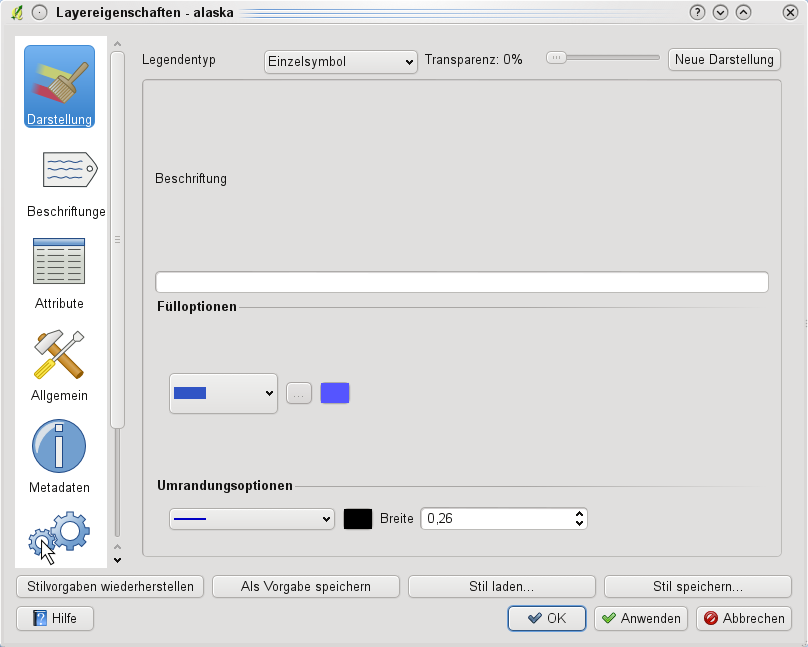
\includegraphics[clip=true, width=0.4\textwidth]{vectorClassifySingle}}\goodgap
  \subfloat[Symbole unique] {\label{subfig:single_symbol}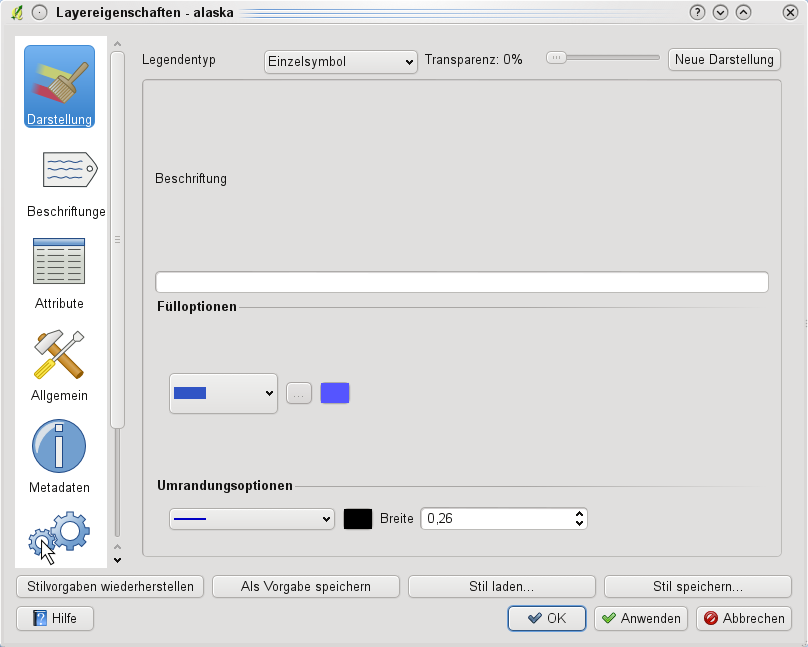
\includegraphics[clip=true, width=0.48\textwidth]{vectorClassifySingle}}
  %\subfigure[Graduated symbol] {\label{subfig:graduated_symbol}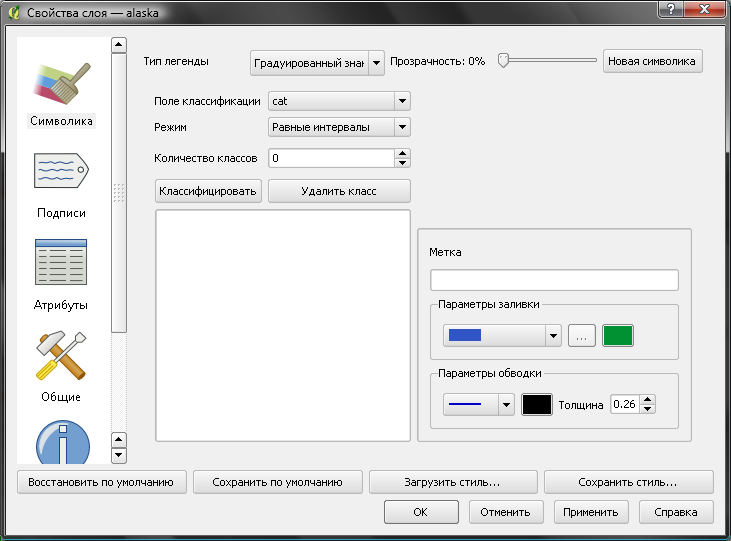
\includegraphics[clip=true, width=0.4\textwidth]{vectorClassifyGraduated}}\\
\hspace{0.1cm}
  \subfloat[Symbole gradué] {\label{subfig:graduated_symbol}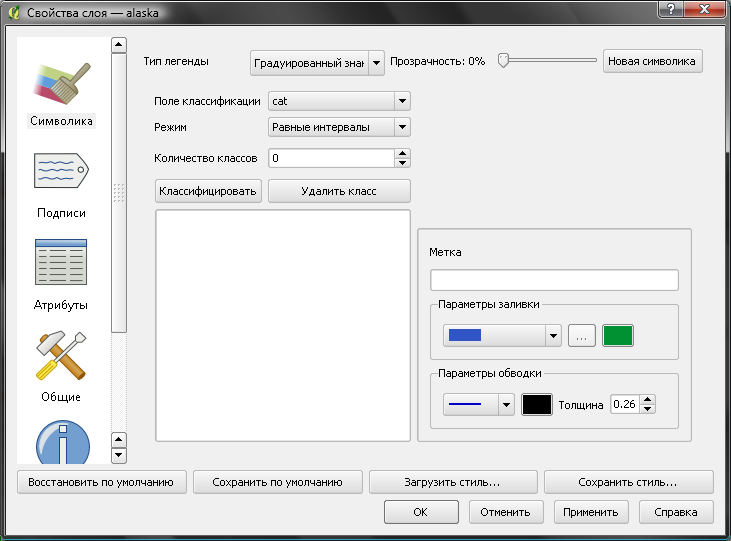
\includegraphics[clip=true, width=0.48\textwidth]{vectorClassifyGraduated}}\\
  %\subfigure[Continous color] {\label{subfig:cont_color}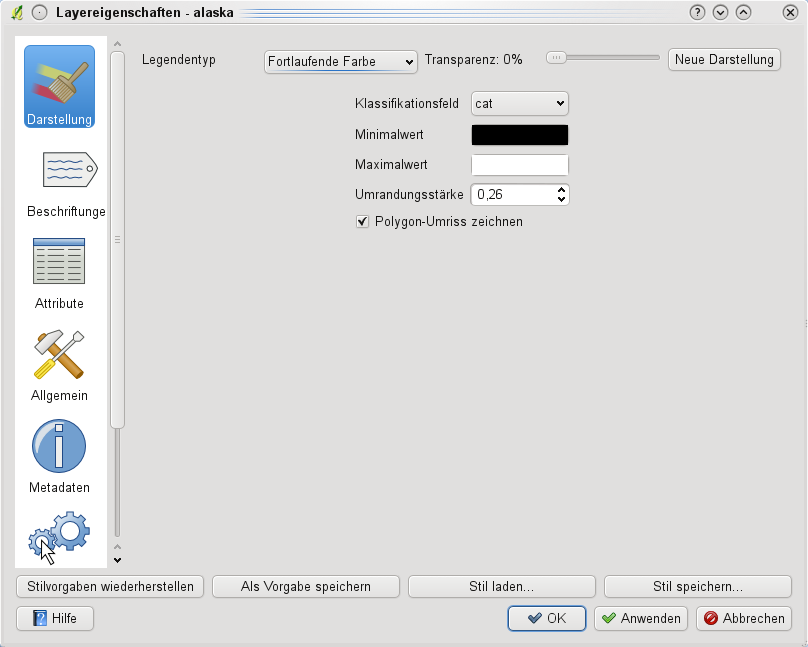
\includegraphics[clip=true, width=0.4\textwidth]{vectorClassifyContinous}}\goodgap
  \subfloat[Couleur continue] {\label{subfig:cont_color}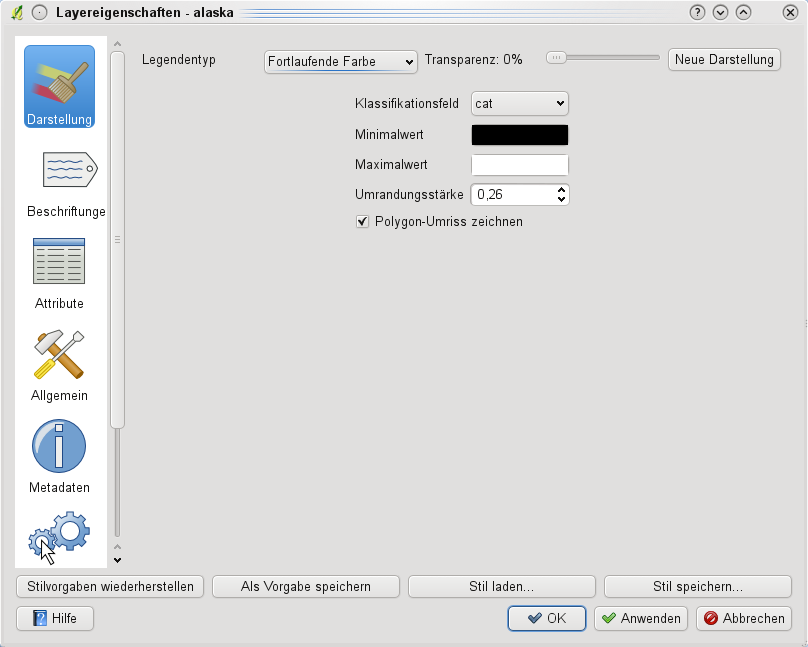
\includegraphics[clip=true, width=0.48\textwidth]{vectorClassifyContinous}}
  %\subfigure[Unique value] {\label{subfig:unique_val}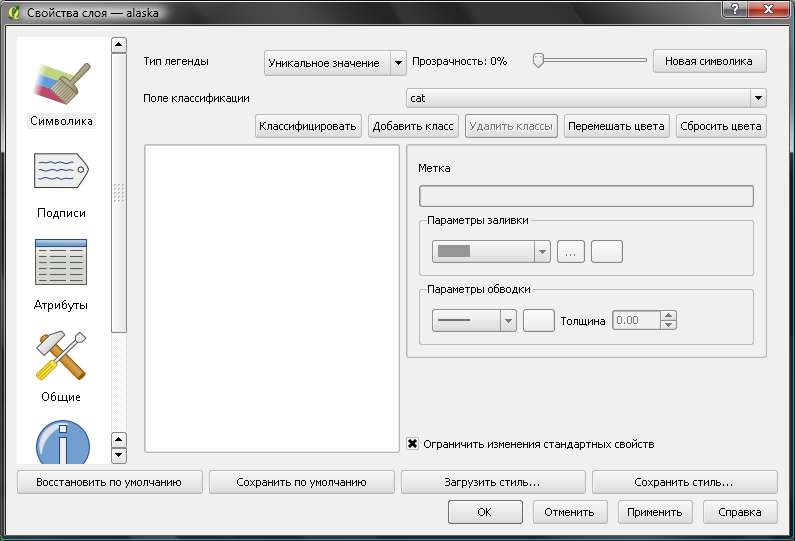
\includegraphics[clip=true, width=0.4\textwidth]{vectorClassifyUnique}}
  \hspace{0.1cm}
  \subfloat[Valeur unique] {\label{subfig:unique_val}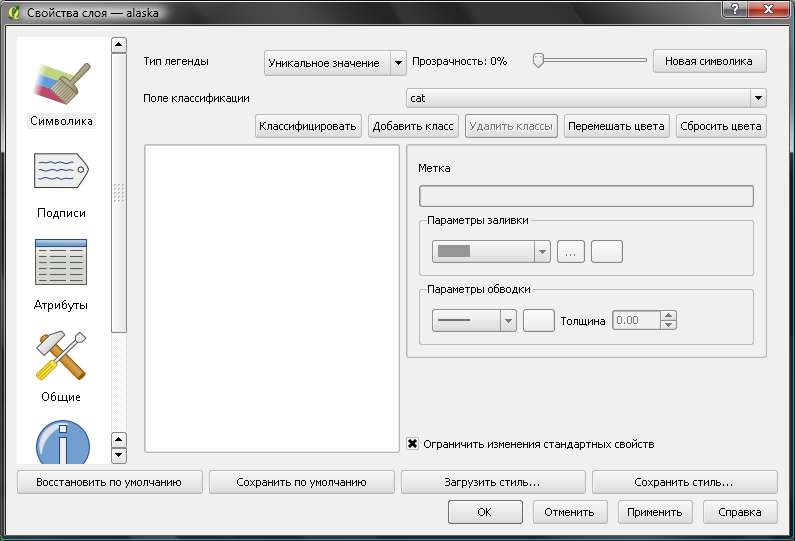
\includegraphics[clip=true, width=0.48\textwidth]{vectorClassifyUnique}}
  \caption{Options de symbolisation \nixcaption}
\end{figure}

% FIXME: outdated
% Since \usertext{version v0.9} there is a function to use image files stored on
% your computer as fill pattern for vector layers.

%\minisec{Style Options} \label{sec:style_options} \index{vector layers!styles}
\minisec{Options de style} \label{sec:style_options}\index{couches vecteur!styles}
%Within this dialog you can style your vector layer. Depending on the selected rendering option you have the possibility to also classify your mapfeatures.
Dans cette fenêtre vous pouvez donner un style à votre couche vecteur. Selon l'option de rendu sélectionnée, vous avez la possibilité de classer vos entités.

%At least the following styling options apply for nearly all renderers:
Les options de style suivantes s'appliquent quasiment à tous les types de rendus :
\begin{description}
%\item[Outline style] - pen-style for your outline of your feature. you can also set this to 'no pen'.
\item[Style du contour :] style de la ligne qui fait le contour de vos entités. Vous pouvez également le définir à \og no pen\fg, pas de contour
%\item[Outline color] - color of the ouline of your feature
\item[Couleur du contour :] couleur du contour de vos entités
%\item[Outline width] - width of your features
\item[Épaisseur du contour :] épaisseur du contour de vos entités
%\item[Fill color] - fill-color of your features.
\item[Couleur de remplissage :] couleur de remplissage de vos entités
%\item[Fill style] - Style for filling. Beside the given brushes you can select \selectstring{Fill style}{? texture} and click the \browsebutton button for selecting your own fill-style. Currently the fileformats \filename{*.jpeg, *.xpm, and *.png} are supported.
\item[Style de remplissage :] Style pour le remplissage. En plus des pinceaux proposés, vous pouvez sélectionner \selectstring{Fill style ? texture} et cliquez sur le \browsebutton bouton pour sélectionner votre propre style de remplissage. Actuellement, les formats de fichier \filename{*.jpeg, *.xpm et *.png}
\end{description}

%Once you have styled your layer you also could save your layer-style to a separate file (with \filename{*.qml}-ending). To do this, use the button \button{Save Style \ldots}. No need to say that \button{Load Style \ldots} loads your saved layer-style-file.
Une fois que vous avez défini le style de votre couche, vous pouvez le sauvegarder dans un fichier séparé (avec l'extension \filename{*.qml}). Pour faire cela, utilisez le bouton \button{Sauvegarder le style \ldots} Inutile de dire que \button{Charger le style \ldots} charge vos fichiers sauvegardés.

%If you wish to always use a particular style whenever the layer is loaded, use the \button{Save As Default} button to make your style the default. Also, if you make changes to the style that you are not happy with, use the \button{Restore Default Styel} button to revert to your default style.
Si vous voulez utiliser en permanence un style particulier chaque fois que la couche est chargée, utilisez le bouton \button{Sauvegarder comme défaut} pour en faire le style par défaut. Aussi, si le style ne vous plait pas et que vous le modifiez, utilisez le bouton \button{Restaurer le style par défaut} pour en faire votre style par défaut.

%\minisec{Vector transparency} \label{sec:vect_transparency} \index{vector layers!transparency}
\minisec{Transparence d'une couche vecteur} \label{sec:vect_transparency} \index{couches vecteur!transparence}
%\qg \CURRENT allows to set a transparency for every vector layer. This can be done with the slider \slider{Transparency}{0}{20mm} inside the \tab{symbology} tab (see fig. \ref{fig:vector_symbology}). This is very useful for overlaying several vector layers.
\qg \CURRENT permet de définir une transparence pour chaque couche vecteur. Ceci peut-être fait avec le curseur \slider{Transparence} de l'onglet \tab{Convention des signes} (voir fig. \ref{fig:vector_symbology}). Ceci est très utile pour superposer plusieurs couches vecteur.

%\subsection{Metadata Tab}
\subsection{Onglet Métadadonnées}

%The \tab{Metadata} tab contains information about the layer, including specifics about the type and location, number of features, feature type, and the editing capabilities. The \guiheading{Layer Spatial Reference System} section, providing projection information, and the \guiheading{Attribute field info} section, listing fields and their data types, are displayed on this tab. This is a quick way to get information about the layer.
L'onglet \tab{Métadadonnées} contient les informations sur la couche dont le type et la localisation, le nombre d'entités, le type des entités et les possibilités d'éditions. Les sections \guiheading{Système spatial de référence de la couche} qui fournit les informations sur la projection et \guiheading{Information de champ d'attribut} qui liste les champs et leur type sont affichées dans cet onglet. Cet onglet constitue un moyen rapide d'obtenir des informations sur une couche.

%\subsection{Labels Tab}
\subsection{Onglet Étiquettes}

%The \tab{Labels} tab allows you to enable labeling features and control a number of options related to fonts, placement, style, alignment and buffering.
L'onglet \tab{Étiquettes} vous permet d'activer la fonctionnalité d'étiquetage et de gérer un certain nombre d'options liées à la police de caractère, au placement, au style, à l'alignement et au buffering.

%We will illustrate this by labelling the lakes shapefile of the \filename{qgis\_example\_dataset}:
Nous allons illustrer tout cela en étiquetant le shapefile des lacs du jeu de données\\ \filename{qgis\_example\_dataset} :

\begin{enumerate}
%\item Load the Shapefile \filename{alaska.shp} and GML file \filename{lakes.gml} in \qg.
\item Charger le shapefile \filename{alaska.shp} et le fichier GML \filename{lakes.gml} dans \qg
%\item Zoom in a bit to your favorite area with some lake.
\item Zoommez légèrement sur votre coin préféré avec quelques lacs
%\item Make the \filename{lakes} layer active.
\item Rendez active la couche \filename{lakes}
%\item Open the \dialog{Layer Properties} dialog.
\item Ouvrez la fenêtre \dialog{Propriétés de la couche}
%\item Click on the \tab{Labels} tab.
\item Cliquez sur l'onglet \tab{Étiquettes}
%\item Check the \checkbox{Display labels} checkbox to enable labeling.
\item Cochez la case \checkbox{Afficher les étiquettes} pour activer l'étiquetage
%\item Choose the field to label with. We'll use \selectstring{Field containing label}{NAMES}.
\item Choisissez le champ à utiliser pour les étiquettes. Ici, nous utiliserons le\\ \selectstring{Champ contenant une étiquette}{NAMES}
%\item Enter a default for lakes that have no name. The default label will be used each time \qg encounters a lake with no value in the \guilabel{NAMES} field.
\item Choisissez un libellé par défaut pour les lacs n'ayant pas de nom. Ce libellé sera utilisé chaque fois que \qg rencontre un lac n'ayant pas de valeur dans le champ \guilabel{NAMES}
\item Si des étiquettes s'étendent sur plusieurs lignes, cochez \checkbox{Etiquettes multilignes ?} \qg cherchera un retour à la ligne dans le champ de l'étiquette pour insérer une rupture en accord. Un véritable retour à la ligne est un caractère \textbf{unique} \textbackslash n, (et non pas 2 caractères séparés comme un antislash \textbackslash ~suivi par un n)
%\item Click \button{Apply}.
\item Cliquez sur \button{Appliquer}
\end{enumerate}

%Now we have labels. How do they look? They are probably too big and poorly placed in relation to the marker symbol for the lakes.
Maintenant, nous avons des étiquettes. De quoi ont-elles l'air ? Elles sont probablement trop grandes et mal placées par rapport au symbole marqueur des lacs.

%Select the \tab{Font} entry and use the \button{Font} and \button{Color} buttons to set the font and color. You can also change the angle and the placement of the text-label.
Sélectionnez l'entrée \tab{Police} et utilisez les boutons \button{Police} et \button{Couleur} pour définir la police et la couleur. Vous pouvez également changer l'angle et le placement de l'étiquette.

%To change the position of the text relative to the feature:
Pour changer la position du texte par rapport à l'entité :

\begin{enumerate}
%\item Click on the \tab{Font} entry.
\item Cliquez sur l'entrée \tab{Police}
%\item Change the placement by selecting one of the radio buttons in the \classname{Placement} group. To fix our labels, choose the \radiobuttonon{Right} radio button.
\item Changer le placement en sélectionnant l'un des boutons radio dans le groupe \classname{Placement}. Pour corriger nos étiquettes, choisissez le bouton radio \radiobuttonon{Droite}
%\item the \classname{Font size units} allows you to select between \radiobuttonon{Points} or \radiobuttonon{Map units}.
\item La \classname{Taille de la police des unités} vous permet de choisir entre  des \radiobuttonon{Points} ou des \radiobuttonon{Unités de carte}
%\item Click \button{Apply} to see your changes without closing the dialog.
\item Cliquez sur \button{Appliquer} pour visualiser les changements sans fermer la fenêtre
\end{enumerate}

%Things are looking better, but the labels are still too close to the marker. To fix this we can use the options on the \tab{Position} entry. Here we can add offsets for the X and Y directions. Adding an X offset of 5 will move our labels off the marker and make them more readable. Of course if your marker symbol or font is larger, more of an offset will be required.
Ça à l'air plus joli, mais les étiquettes sont encore trop proches des marqueurs. Pour corriger cela, nous pouvons utiliser les options de l'entrée \tab{Position}. Ici, nous pouvons ajouter un décalage dans les directions X et Y. Ajouter un décalage de 5 en X déplacera vos étiquettes et les rendra plus lisibles. Bien sûr si vos symboles marqueurs ou votre police sont plus grands un décalage plus important sera nécessaire.

%The last adjustment we'll make is to \tab{buffer} the labels. This just means putting a backdrop around them to make them stand out better. To buffer the lakes labels:
Un dernier ajustement reste à faire sur les étiquettes : un \tab{tampon}. Il s'agit de créer un fond autour des étiquettes pour les faire mieux ressortir. Pour faire un tampon sur les étiquettes des lacs :

\begin{enumerate}
%\item Click the \tab{Buffer} tab.
\item Cliquez sur l'entrée \tab{Tampon}
%\item Click the \checkbox{Buffer Labels?} checkbox to enable buffering.
\item Cliquez sur la case à cocher \checkbox{Tampon d'éitquette ?} pour activer le tampon
%\item Choose a size for the buffer using the spin box.
\item Choisissez une taille de tampon en utilisant les flèches
%\item Choose a color by clicking on \button{Color} and choosing your favorite from the color selector. You can also set some transparency for the  buffer if you prefer.
\item Choisissez une couleur en cliquant sur \button{Couleur} puis choisissez votre couleur favorite grâce au sélecteur. Si vous le souhaitez, vous pouvez également ajouter un peu de transparence au tampon
%\item Click \button{Apply} to see if you like the changes.
\item Cliquez sur \button{Appliquer} pour voir si les changements vous plaisent
\end{enumerate}

%If you aren't happy with the results, tweak the settings and then test again by clicking \button{Apply}.
Si le résultat ne vous plaît pas, ajustez les paramètres et re-testez en cliquant sur \button{Appliquer}

%A buffer of 1 points seems to give a good result. Notice you can also specify the buffer size in map units if that works out better for you.
Le tampon d'une taille d'un point semble donner un bon résultat. Notez que vous pouvez également spécifier une taille de tampon en unités de la carte si cela vous convient mieux.

%The remaining entries inside the \tab{Label} tab allow you control the appearance of the labels using attributes stored in the layer. The entries beginning with \tab{Data defined} allow you to set all the parameters for the labels using fields in the layer.
Les autres entrées de l'onglet \tab{Étiquettes} vous permettent de contrôler l'apparence des étiquettes en utilisant les attributs stockés dans la couche. Les entrées commençantes par \tab{Data defined} vous permettent de définir tous les paramètres des étiquettes en utilisant des champs de la couche.

%Not that the \tab{Label} tab provides a \classname{preview-box} where your selected label is shown.
Notez que l'onglet \tab{Étiquettes} propose une \classname{Prévisualisation} montrant une de vos étiquettes.

%\subsection{Actions Tab}\index{actions}\label{label_actions}
\subsection{Onglet Actions}\index{actions}\label{label_actions}

%\qg provides the ability to perform an action based on the attributes of a feature. This can be used to perform any number of actions, for example, running a program with arguments built from the attributes of a feature or passing parameters to a web reporting tool.
\qg est capable d'effectuer des actions basées sur les attributs d'une entité. Il peut s'agir de nombreuses actions, par exemple exécuter un programme avec des arguments construits à partir des attributs d'une entité, ou encore, passer des paramètres à un outil de publication de rapports sur internet.

%Actions are useful when you frequently want to run an external application or view a web page based on one or more values in your vector layer. An example is performing a search based on an attribute value. This concept is used in the following discussion.
Les actions sont utiles si vous voulez exécuter fréquemment une application externe ou charger une page web basée sur une ou plusieurs valeurs de votre couche vecteur. Un exemple d'application serait d'effectuer une recherche basée sur une valeur d'attribut. C'est l'idée utilisée dans les paragraphes qui suivent.

%\minisec{Defining Actions}\index{actions!defining}
\minisec{Définir des actions}\index{actions!définir}

%Attribute actions are defined from the vector \dialog{Layer Properties} dialog. To define an action, open the vector \dialog{Layer Properties} dialog and click on the \tab{Actions} tab. Provide a descriptive name for the action. The action itself must contain the name of the application that will be executed when the action is invoked. You can add one or more attribute field values as arguments to the application. When the action is invoked any set of characters that start with a \% followed by the name of a field will be replaced by the value of that field. The special characters \%\% \index{\%\%}will be replaced by the value of the field that was selected from the identify results or attribute table (see Using Actions below).  Double quote marks can be used to group text into a single argument to the program, script or command. Double quotes will be ignored if preceded by a backslash.
Les actions sur les attributs sont définies dans la fenêtre \dialog{Propriétés de la couche} des couches vecteur. Pour définir une action, ouvrez la fenêtre de \dialog{Propriétés de la couche} et cliquez sur l'onglet \tab{Actions}. Donnez un nom descriptif à l'action. L'action elle-même doit contenir le nom de l'application qui sera exécutée quand l'action sera invoquée. Vous pouvez ajouter un ou plusieurs champs d'attributs comme argument pour l'application. Quand l'action est invoquée n'importe quelle chaîne de caractère précédée de \% et correspondant au nom d'un champ sera remplacé par la valeur de ce champ. Le caractère spécial \%\% \index{\%\%} sera remplacé par la valeur d'un champ qui a été sélectionné par le résultat d'un Identifier ou dans la table d'attributs (voir Utiliser les actions, ci-dessous). Des guillemets peuvent être utilisés pour grouper du texte en un seul argument pour le programme, le script ou la commande. Les guillemets seront ignorés s'ils sont précédés d'un antislash.

%If you have field names that are substrings of other field names (e.g., \usertext{col1} and \usertext{col10}) you should indicate so, by surrounding the field name (and the \% character) with square brackets (e.g., \usertext{[\%col10]}). This will prevent the \usertext{\%col10} field name being mistaken for the \usertext{\%col1} field name with a \usertext{0} on the end. The brackets will be removed by \qg when it substitutes in the value of the field. If you want the substituted field to be surrounded by square brackets, use a second set like this: \usertext{[[\%col10]]}.
Si vous avez des noms de champs qui sont contenus dans d'autres noms de champs (par exemple, \usertext{col1} et \usertext{col10}), vous devez l'indiquer en entourant le nom de champ (le caractère \%) par des crochets (par exemple \usertext{[\%col10]}). Ceci évitera de prendre le nom de champ \usertext{\%col10} pour \usertext{\%col1} avec un \usertext{0} à la fin. Les crochets seront retirés quand \qg substituera le nom par la valeur du champ. Si vous voulez que le champ à substituer soit entouré de crochets, utilisez un deuxième jeu de crochets comme ici : \usertext{[[\%col10]]}.

%The \dialog{Identify Results} dialog box includes a {\em (Derived)} item that contains information relevant to the layer type. The values in this item can be accessed in a similar way to the other fields by using preceeding the derived field name by \usertext{(Derived).}. For example, a point layer has an \usertext{X} and \usertext{Y} field and the value of these can be used in the action with \usertext{\%(Derived).X} and \usertext{\%(Derived).Y}. The derived attributes are only available from the \dialog{Identify Results} dialog box, not the \dialog{Attribute Table} dialog box.
La fenêtre \dialog{Résultats identifiés} inclut une entrée {\em (Dérivé)} qui contient des informations pertinentes selon le type de couche. Les valeurs de cette entrée sont accessibles de la même manière que les autres champs en ajoutant \usertext{(Derived).} avant le nom du champ. Par exemple, une couche de points à un champ \usertext{X} et \usertext{Y} et leur valeur peut être utilisée dans l'action avec \usertext{\%(Derived).X} et \usertext{\%(Derived).Y}. Les attributs dérivés sont disponibles uniquement depuis la fenêtre \dialog{Résultats identifiés} et pas la \dialog{Table d'attributs}.

%Two example actions are shown below:\index{actions!examples}
Deux exemples d'action sont proposés ci-dessous : \index{actions!exemples}

\begin{itemize}[label=--]
  \item \usertext{konqueror http://www.google.com/search?q=\%nam}
  \item \usertext{konqueror http://www.google.com/search?q=\%\%}
\end{itemize}

%In the first example, the web browser konqueror is invoked and passed a URL to open. The URL performs a Google search on the value of the \usertext{nam} field from our vector layer. Note that the application or script called by the action must be in the path or you must provided the full path. To be sure, we could rewrite the first example as: \usertext{/opt/kde3/bin/konqueror http://www.google.com/search?q=\%nam}. This will ensure that the konqueror application will be executed when the action is invoked.
Dans le premier exemple, le navigateur internet konqueror est lancé avec une URL. L'URL effectue une recherche Google sur la valeur du champ \usertext{nam} de la couche vecteur. Notez que l'application ou le script appelé par l'action doit être dans le path sinon vous devez fournir le chemin complet vers l'application. Pour être certain, nous pouvons réécrire le premier exemple de cette manière : \usertext{/opt/kde3/bin/konqueror http://www.google.com/search?q=\%nam}. Ceci assurera que l'application konqueror sera exécutée quand l'action sera invoquée.

%The second example uses the \%\% notation which does not rely on a particular field for its value. When the action is invoked, the \%\% will be replaced by the value of the selected field in the identify results or attribute table.
Le deuxième exemple utilise la notation \%\% dont la valeur ne dépend pas d'un champ en particulier. Quand l'action est invoquée, \%\% sera remplacé par la valeur du champ sélectionné dans les résultats de l'identification ou dans la table d'attributs.

%\minisec{Using Actions}\index{actions!using}\label{label_usingactions}
\minisec{Utiliser les actions}\index{actions!utiliser}\label{label_usingactions}
%Actions can be invoked from either the \dialog{Identify Results} dialog or an \dialog{Attribute Table} dialog. (Recall that these dialogs can be opened by clicking \toolbtntwo{mActionOpenTable}{Identify Features} or \toolbtntwo{mActionOpenTable}{Open Table}.)
Les actions peuvent être invoquées soit depuis la fenêtre \dialog{Résultats identifiés} soit depuis la \dialog{Table d'attributs}. (Rappelez-vous que ces fenêtres s'ouvrent en cliquant sur\\ \toolbtntwo{mActionOpenTable}{Identifier les données} ou \toolbtntwo{mActionOpenTable}{Ouvrir la table d'attributs}.)
%To invoke an action, right click on the record and choose the action from the popup menu. Actions are listed in the popup menu by the name you assigned when defining the actions. Click on the action you wish to invoke.
Pour invoquer une action, faites un clic droit sur un enregistrement et choisissez l'action depuis le menu qui apparaît. Les actions sont listées dans le menu par le nom que vous leur avez donné en les définissant. Cliquez ensuite sur l'action que vous souhaitez invoquer.

%If you are invoking an action that uses the \%\% notation, right-click on the field value in the \dialog{Identify Results} dialog or the \dialog{Attribute Table} dialog that you wish to pass to the application or script.
Si vous invoquez une action qui utilise la notation \%\%, faites un clic droit sur la valeur du champ que vous souhaitez passer en argument à l'application ou au script dans la fenêtre \dialog{Résultats identifiés} ou la \dialog{Table d'attributs}.

%Here is another example that pulls data out of a vector layer and inserts them into a file using bash and the \usertext{echo} command (so it will only work \nix or perhaps \osx). The layer in question has fields for a species name \usertext{taxon\_name}, latitude \usertext{lat} and longitude \usertext{long}. I would like to be able to make a spatial selection of a localities and export these field values to a text file for the selected record (shown in yellow in the \qg map area). Here is the action to achieve this:
Voici un autre exemple qui récupère des données d'une couche vecteur et qui les insère dans un fichier utilisant bash et la commande \usertext{echo} (cela ne marchera que sur \nix et peut-être \osx). La couche en question à des champs pour le nom d'espèce \usertext{taxon\_name}, la latitude \usertext{lat} et la longitude \usertext{long}. Je souhaiterais faire une sélection spatiale des localités et exporter ces valeurs des enregistrements sélectionnés dans un fichier texte (ils apparaissent en jaune sur la carte dans \qg). Voici l'action qui permettra de le faire :

\begin{verbatim}
  bash -c "echo \"%taxon_name %lat %long\" >> /tmp/species_localities.txt"
\end{verbatim}

%After selecting a few localities and running the action on each one, opening the output file will show something like this:
Après avoir sélectionné quelques localités et lancé l'action sur chacune, le fichier de destination ressemblera à ça :

\begin{verbatim}
  Acacia mearnsii -34.0800000000 150.0800000000
  Acacia mearnsii -34.9000000000 150.1200000000
  Acacia mearnsii -35.2200000000 149.9300000000
  Acacia mearnsii -32.2700000000 150.4100000000
\end{verbatim}

%As an exercise we create an action that does a Google search on the \filename{lakes} layer. First we need to determine the URL needed to perform a search on a keyword. This is easily done by just going to Google and doing a simple search, then grabbing the URL from the address bar in your browser. From this little effort we see that the format is: \url{http://google.com/search?q=qgis}, where \usertext{qgis} is the search term. Armed with this information, we can proceed:
Comme exercice, nous allons créer une action qui réalise une recherche Google sur la couche \filename{lakes}. Tout d'abord, nous avons besoin de déterminer l'URL nécessaire pour effectuer une recherche sur un mot clé. Il suffit simplement d'aller sur Google et faire une recherche simple puis récupérer l'URL dans la barre d'adresse de votre navigateur. De cela, nous en déduisons la formulation : \url{http://google.com/search?q=qgis}, où \usertext{qgis} est le terme recherché. À partir de tout cela, nous pouvons poursuivre :

\begin{enumerate}
%\item Make sure the \filename{lakes} layer is loaded.
\item Assurez-vous que la couche \filename{lakes} est chargée
%\item Open the \dialog{Layer Properties} dialog by double-clicking on the layer in the legend or right-click and choose \dropmenuopt{Properties} from the popup menu.
\item Ouvrez la fenêtre \dialog{Propriétés de la couche} en double cliquant sur la couche dans la légende ou en faisant un clic droit et en choisissant \dropmenuopt{Propriétés} dans le menu qui apparaît
%\item Click on the \tab{Actions} tab.
\item Cliquez sur l'onglet \tab{Actions}
%\item Enter a name for the action, for example \usertext{Google Search}.
\item Entrez un nom pour l'action, par exemple \usertext{Recherche Google}
%\item For the action, we need to provide the name of the external program to run. In this case, we can use Firefox. If the program is not in your path, you need to provide the full path.
\item Pour l'action, nous devons fournir le nom du programme externe à lancer. Dans ce cas, nous allons utiliser Firefox. Si le programme n'est pas dans votre path, vous devez fournir le chemin complet
%\item Following the name of the external application, add the URL used for doing a Google search, up to but not included the search term:  \url{http://google.com/search?q=}
\item A la suite du nom de l'application externe, ajoutez l'URL utilisée pour faire la recherche Google, jusqu'au terme de recherche, mais sans l'ajouter :\\ \url{http://google.com/search?q=}
%\item The text in the \guilabel{Action} field should now look like this:\\
%\usertext{firefox \url{http://google.com/search?q=}}
\item Le texte dans le champ \guilabel{Action} devrait ressembler à ça :\\
\usertext{firefox \url{http://google.com/search?q=}}
%\item Click on the drop-down box containing the field names for the \usertext{lakes} layer. It's located just to the left of the \button{Insert Field} button.
\item Cliquez sur le menu déroulant contenant les noms des champs pour la couche \usertext{lakes}. Il est situé juste à gauche du bouton \button{Insérer un champ}
%\item From the drop-down box, select \selectstring{}{NAMES} and click \button{Insert Field}.
\item Dans le menu déroulant, sélectionnez \selectstring{NAMES} et cliquez sur \button{Insérer un champ}
%\item Your action text now looks like this:\\
%\usertext{firefox \url{http://google.com/search?q=\%NAMES}}
\item Le texte de votre action devrait maintenant ressembler à ça :\\
\usertext{firefox \url{http://google.com/search?q=\%NAMES}}
%\item Fo finalize the action click the \button{Insert action} button..
\item Pour finaliser l'action, cliquez sur le bouton \button{Insérer une action}
\end{enumerate}

%This completes the action and it is ready to use. The final text of the action should look like this:
L'action est donc entièrement définie et prête à être utilisée. Le texte final de l'action devrait correspondre à ça :

\begin{center}
\usertext{firefox \url{http://google.com/search?q=\%NAMES}}
\end{center}

%We can now use the action. Close the \dialog{Layer Properties} dialog and zoom in to an area of interest. Make sure the \filename{lakes} layer is active and identify a lake. In the result box you'll now see that our action is visible:
Nous pouvons maintenant utiliser l'action. Fermez la fenêtre \dialog{Propriétés de la couche} et zoomez sur une zone d'intérêt. Assurez-vous que la couche \filename{lakes} est active puis identifiez un lac. Dans la fenêtre de résultats, vous constatez que notre action est maintenant visible :

\begin{figure}[H]
  \begin{center}
  %\caption{Select feature and choose action \nixcaption}\label{fig:identify_action}\smallskip
  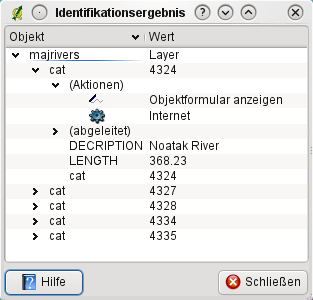
\includegraphics[clip=true, width=8cm]{action_identifyaction}
  \caption{Sélectionnez une entité et choisissez une action \nixcaption}\label{fig:identify_action}
\end{center}
\end{figure}

%When we click on the action, it brings up Firefox and navigates to the URL \url{http://www.google.com/search?q=Tustumena}. It is also possible to add further attribute fields to the action. Therefore you can add a ``+'' to the end of the action text, select another field and click on \button{Insert Field}. In this example there is just no other field available that would make sense to search for.
Quand vous cliquez sur l'action, cela ouvre Firefox et charge l'URL \url{http://www.google.com/search?q=Tustumena}. Il est également possible d'ajouter d'autres champs attributs à l'action. Pour faire cela, vous pouvez ajouter un \og +\fg à la fin du texte de l'action, sélectionnez un autre champ et cliquez sur \button{Insérer un champ}. Dans cet exemple, la recherche sur un autre champ n'aurait pas de sens.

%You can define multiple actions for a layer and each will show up in the \dialog{Identify Results} dialog. You can also invoke actions from the attribute table by selecting a row and right-clicking, then choosing the action from the popup menu.
Vous pouvez définir de multiples actions pour une couche et chacune apparaitra dans la fenêtre \dialog{Résultats identifiés}. Vous pouvez également invoquer des actions depuis la table d'attributs en sélectionnant une colonne et en faisant un clic droit puis en choisissant l'action dans le menu qui apparaît.

%You can think of all kinds of uses for actions. For example, if you have a point layer containing locations of images or photos along with a file name, you could create an action to launch a viewer to display the image. You could also use actions to launch web-based reports for an attribute field or combination of fields, specifying them in the same way we did in our Google search example.
Vous pouvez imaginer toute sorte d'utilisations pour ces actions. Par exemple, si vous avait une couche de points contenant la localisation d'images ou de photos ainsi qu'un nom de fichier, vous pouvez créer une action qui lancera un visualisateur pour afficher les images. Vous pouvez également utiliser les actions pour lancer des rapports sur internet pour un champ attributaire ou une combinaison de champs, en les spécifiant de la même manière que pour une recherche

%\subsection{Attributes Tab}\index{attributes}\label{label_attributes}
\subsection{Onglet attributs}\index{attributs}\label{label_attributes}
%Within the \tab{Attributes} tab the attributes of the selected dataset can be manipulated. The buttons \toolbtntwo{mActionNewAttribute}{New Column} and \toolbtntwo{mActionDeleteAttribute}{Delete Column} can be used, when the dataset is \toolbtntwo{mActionToggleEditing}{editing mode}. At the moment only columns from \pg layers can be removed and added. The OGR library supports to add new columns, but not to remove them, if you have a GDAL version >= 1.6 installed. 
Dans l'onglet \tab{Attributs}, il est possible de manipuler les attributs du jeu de données sélectionné. Les boutons \toolbtntwo{mActionNewAttribute}{Ajouter une colonne} et \toolbtntwo{mActionDeleteAttribute}{Supprimer une colonne} peuvent être utilisés lorsque le jeu de données est en mode édition. Actuellement, seules les colonnes des couches \pg peuvent être effacées ou ajoutées. La bibliothèque OGR, dans les versions $\geq$ à la 1.6, supporte l'ajout de nouvelles colonnes, mais pas la suppression.

%The \button{Toggle editing mode} button toggles this mode.
Le bouton \button{Basculer en mode édition} permet de passer dans ce mode.

%\minisec{edit widget}
\minisec{Outils d'édition}

\begin{figure}[H]
   \begin{center}
   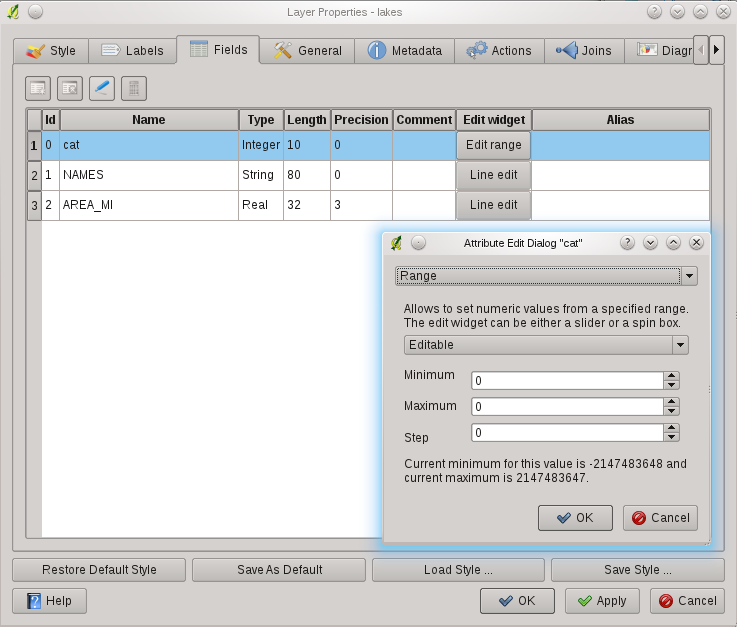
\includegraphics[clip=true, width=12cm]{editwidgetsdialog}
   \caption{Dialogue pour la sélection d'un widget d'édition pour une colonne attributaire \nixcaption}\label{fig:editwidget}
\end{center}
\end{figure}

%Within the \tab{Attributes} tab you also find an \texttt{edit widget} and a \texttt{value} column. These two columns can be used to define values or a range of values that are allowed to be added to the specific attribute table columns. They are used to produce different edit widgets in the attribute dialog. These widgets are:
Dans l'onglet \tab{Attributs} vous trouverez un colonne \texttt{Outils d'édition} et une colonne \texttt{valeur}. Ces deux colonnes peuvent être utilisées pour définir les valeurs ou les plages de valeurs permises lors de l'ajout d'attributs dans une colonne. Elles sont utilisées pour générer différents outils d'édition dans la fenêtre des attributs. Ces outils sont :
\begin{itemize}[label=--]
\item édition de ligne : un champ d'édition qui permet d'entrer du texte simple (ou de restreindre à des nombres pour des attributs de type numériques)
%\item Classification: Displays a combo box with the values used for classification, if you have chosen 'unique value' as legend type in the symbology tab of the properties dialog.
\item Classification : Affiche une boîte combo avec les valeurs utilisées pour la classification, si vous avez choisi \og valeur unique\fg comme type de légende dans la symbologie
%\item Range: Allows to set numeric values from a specific range. The edit widget can be either a slider or a spin box.
\item Portée : Permet d'indiquer des valeurs numériques depuis une portée spécifiée. L'outil d'édition peut être une barre coulissante ou une spinbox
%\item Unique value: The user can select one of the values already used in the attribute table. If editable is activated, a line edit is shown with autocompletion support, otherwise a combo box is used.
\item valeurs uniques : l'utilisateur peut sélectionner une des valeurs déjà utilisées dans la table attributaire. Si l'édition est activée, une ligne est affichée avec le support de l'autocomplétition, autrement une boîte est utilisée
%\item File name: Simplifies the selection by adding a file chooser dialog.
\item nom de fichier : Simplifie la sélection par l'ajout d'un dialogue de sélection de fichier.
%\item Value map: a combo box with predefined items. The value is stored in the attribute, the description is shown in the comboo box. You can define values manually or load them from a layer or a csv file. 
\item Carte de valeur : une boîte combo avec des objets prédéfinis. La valeur peut être stocké dans l'attribut, la description est montrée dans la boîte combo. Vous pouvez définir les valeurs manuellement ou les charger depuis une couche ou un fichier csv
%\item Enumeration: Opens a combo box with values that can be used within the columns type. This is currently only supported by the postgres provider.
\item Enumération : Ouvre une boîte combo avec des valeurs qui peut être utilisé dans le tpe des colonnes. Seul le prestataire postgres le supporte pour l'instant
%\item Immutable: The immutable attribute column is read-only. The user is not able to modify the content. 
\item Immuable : L'attribut immuable est en lecture seule, l'utilisateur ne peut pas modifié le contenu
\end{itemize}

\subsection{Diagramme}\label{sec:diagram}
\index{couches vecteurs!diagramme}
L'onglet \tab{Diagramme} permet d'ajouter une couche de graphiques sur une couche vecteur. Pour activer cette fonctionnalité, ouvrez le gestionnaire d'extension pour y sélectionner l'extension Diagramme Incrusté. Après ça, un nouvel onglet apparaît dans les \dialog{Propriétés de couches} vecteurs où les paramètres de diagrammes peuvent être saisis (voir figure~\ref{fig:diagramtab}).

\begin{figure}[ht]
   \begin{center}
   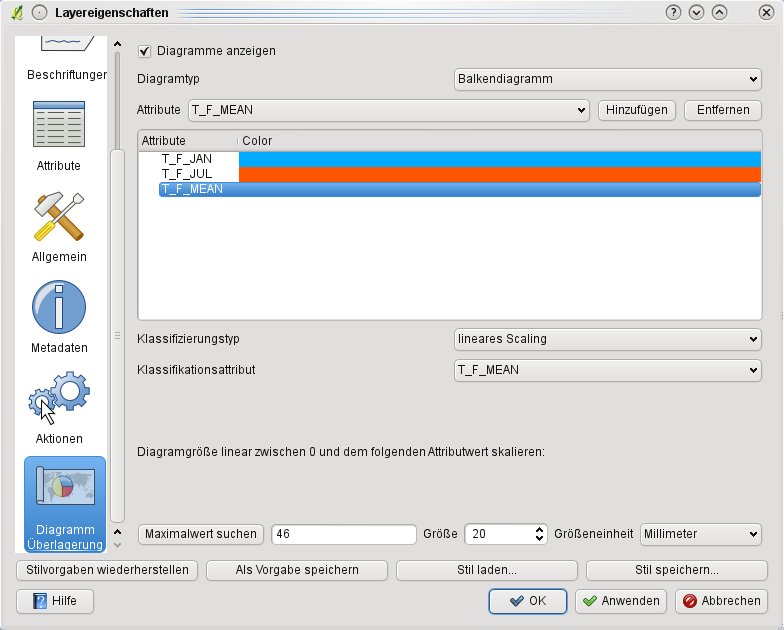
\includegraphics[clip=true, width=12cm]{diagram_tab}
   \caption{Dialogue des propriétés de diagrammes \nixcaption}\label{fig:diagramtab}
\end{center}
\end{figure}

L'implémentation actuelle des diagrammes permet de visualiser des graphiques sous forme de camemberts, de barres ou de lignes selon la valeur d'un attribut de classification. Nous allons vous montrer un exemple en incrustant dans les frontières de l'Alaska des données concernant la température issues d'une couche vecteur portant sur le climat. Toutes ces couches sont disponibles dans l'échantillon de données \qg (voir section~\ref{label_sampledata}).

\begin{enumerate}
\item Cliquez sur l'icône \toolbtntwo{mActionAddOgrLayer}{Ajouter une couche vecteur}, parcourez le répertoire de l'échantillon \qg et chargez \filename{alaska.shp} and \filename{climate.shp}
\item Double-cliquez sur la couche \filename{climate} dans la légende pour ouvrir la fenêtre de\\ \dialog{Propriétés de la Couche}
\item Cliquez sur l'onglet de \tab{Diagramme Incrusté} et sélectionnez \button{Diagramme en barre} comme type de diagramme
\item Nous cherchons à représenter les valeurs de trois colonnes \filename{T\_F\_JAN, T\_F\_JAN} and \filename{T\_F\_MEAN}. Sélectionnez d'abord \filename{T\_F\_JAN} dans la liste des attributs puis cliquez sur \button{Ajouter attribut} ensuite \filename{T\_F\_JUL} et enfin \filename{T\_F\_MEAN}
\item Pour une mise à l'échelle linéaire de la taille du diagramme, nous définissons \filename{T\_F\_JUL} comme étant l'attribut de classification
\item Maintenant cliquez sur \button{Trouver la valeur maximale}, choisissez une valeur de taille et une unité puis cliquez sur \button{Appliquer} pour afficher le diagramme dans la fenêtre principale
\item Vous pouvez adapter la taille du diagramme ou changer la couleur des attributs en double-cliquant sur les valeurs colorimétriques dans la liste attributaire. La figure~\ref{fig:climatediagram} vous donnes une impression du résultat
\item Et pour finir cliquez \button{Ok}.
\end{enumerate}

\begin{figure}[ht]
   \begin{center}
   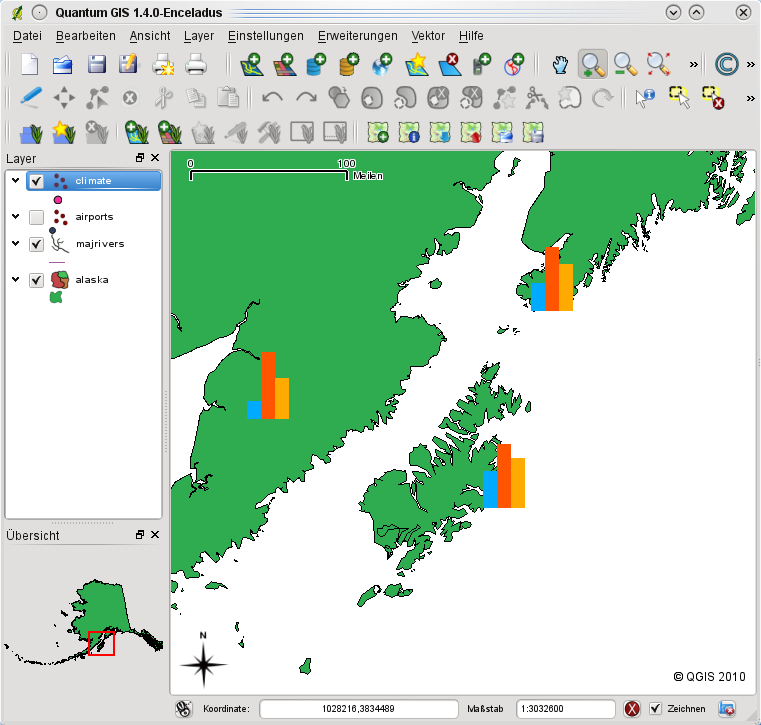
\includegraphics[clip=true, width=12cm]{climate_diagram}
   \caption{Diagramme des températures superposé sur une carte \nixcaption}\label{fig:climatediagram}
\end{center}
\end{figure}

%\section{Editing}\index{editing}
\section{Éditer}\index{éditer}

%\qg supports basic capabilities for editing vector geometries.  Before reading any further you should note that at this stage editing support is still preliminary. Before performing any edits, always make a backup of the dataset you are about to edit.
Les capacités d'édition de \qg sur les géométries vecteur sont basiques. Avant d'aller plus loin, notez que la gestion de l'édition dans \qg reste encore préliminaire. Avant d'effectuer des éditions, créez toujours une sauvegarde du jeu de données que vous allez éditer.

%\textbf{Note} - the procedure for editing GRASS layers is different - see Section \ref{grass_digitising} for details.
\textbf{Note} - la procédure pour éditer des couches GRASS est différente - voir Section \ref{grass_digitising} pour plus de détails.

%\begin{Tip}[ht]\caption{\textsc{Concurrent Edits}}
%\qgistip{This version of \qg does not track if somebody else is editing a
%feature at the same time as you. The last person to save their edits wins.
%}
%\end{Tip}

\begin{Tip}[ht]\caption{\textsc{Éditions concurrentes}}
Cette version de \qg ne vérifie pas si quelqu'un d'autre est en train d'éditer une entité en même temps que vous, la dernière personne qui enregistre gagne.
\end{Tip}

%\subsubsection{Setting the Snapping Tolerance and Search Radius}\label{snapping_tolerance}
\subsubsection{Définir le rayon de tolérance d'accrochage et de recherche}\label{snapping_tolerance}

%Before we can edit vertices, it is very important to set the snapping tolerance and search radius to a value that allows us an optimal editing of the vector layer geometries.
Avant de pouvoir éditer des sommets, il est très important de fixer la tolérance d'accrochage et le rayon de recherche à des valeurs qui nous permettent d'éditer les géométries vecteur de manière optimale.

%\minisec{Snapping tolerance}
\minisec{Tolérance d'accrochage}

%Snapping tolerance is the distance \qg uses to \usertext{search} for the closest vertex and/or segment you are trying to connect when you set a new vertex or move an existing vertex. If you aren't within the snap tolerance, \qg will leave the vertex where you release the mouse button, instead of snapping it to an existing vertex and/or segment.
La tolérance d'accrochage est la distance que \qg utilise pour \usertext{chercher} le sommet ou le segment le plus près que vous cherchez à connecter lorsque vous créez un nouveau sommet ou en déplacez un existant. Si vous n'êtes pas dans la tolérance d'accrochage, \qg va laisser le vertex à l'endroit où vous lâchez le bouton de la souris, au lieu de l'accrocher à un sommet ou un segment existant.

\begin{enumerate}
%\item A general, project wide snapping tolerance can be defined choosing \mainmenuopt{Settings} > \dropmenuopttwo{mActionOptions}{Options}. In the \tab{Digitizing} tab you can select between to vertex, to segment or to vertex and segment as default snap mode. You can also define a default snapping tolerance and a search radius for vertex edits. Remember the tolerance is in layer units. In our digitizing project (working with the Alaska dataset), the units are in feet. Your results may vary, but something on the order of 300ft should be fine at a scale of 1:10 000 should be a reasonable setting.
\item Une tolérance générale, commune à tout le projet, peut-être définie dans \mainmenuopt{Préférences} > \dropmenuopttwo{mActionOptions}{Options}. Dans l'onglet \tab{Numérisation}, vous pouvez choisir le mode d'accrochage par défaut : sur un sommet, sur un segment ou sur un sommet ou un segment. Vous pouvez également définir une tolérance d'accrochage par défaut et un rayon de recherche pour les éditions de sommets. La tolérance peut être définie dans l'unité de la couche ou en pixel, l'avantage du pixel est qu'elle n'a pas à être changée pour tenir compte des zooms. Dans notre projet de numérisation (le travail sur le jeu de données Alaska), les unités sont en pieds. Le résultat peut varier, mais une tolérance de l'ordre de 300 pieds devrait être convenable pour une échelle de 1:\numprint{10000}\ieme
%\item A layer based snapping tolerance can be defined by choosing \mainmenuopt{Settings} > \dropmenuopttwo{mActionOptions}{Project Properties\dots}. In the \tab{General} tab, section \classname{Digitize} you can click on \button{Snapping options\dots} to enable and adjust snapping mode and tolerance on a layer basis (see Figure~\ref{fig:snappingoptions}).
\item Une tolérance d'accrochage liée à une couche peut être définie dans \mainmenuopt{Préférences} > \dropmenuopttwo{mActionOptions}{Propriétés du projet\dots}. Dans l'onglet \tab{Général}, section \classname{Numériser}, vous pouvez cliquer sur \button{Options d'accrochage\dots} pour activer et ajuster le mode d'accrochage et la tolérance pour chaque couche  (voir Figure~\ref{fig:snappingoptions})
\end{enumerate}

%Note that this layer based snapping overrides the global snapping option set in the Digitizing tab. So if you need to edit one layer, and snap its vertices to another layer, then enable snapping only on the \usertext{snap to} layer, then decrease the global snapping tolerance to a smaller value.  Furthermore, snapping will never occur to a layer which is not checked in the snapping options dialog, regardless of the global snapping tolerance. So be sure to mark the checkbox for those layers that you need to snap to.

Veuillez noter que l'accrochage défini pour cette couche est prioritaire par rapport à celui défini dans les options générales. Si vous avez besoin d'éditer une couche en vous accrochant à une autre, il vous faut donc activer l'accrochage uniquement sur la couche à accrocher et réduire la tolérance générale d'accrochage à une valeur moindre. De plus, l'accrochage ne se produira jamais sur une couche dont l'accrochage n'a pas été activé, qu'importe l'option générale. Assurez-vous de cocher la case idoine sur les couches que vous voulez pouvoir utiliser.

\begin{figure}[H]
  \begin{center}
  %\caption{Edit snapping options on a layer basis \nixcaption}\label{fig:snappingoptions}\smallskip
  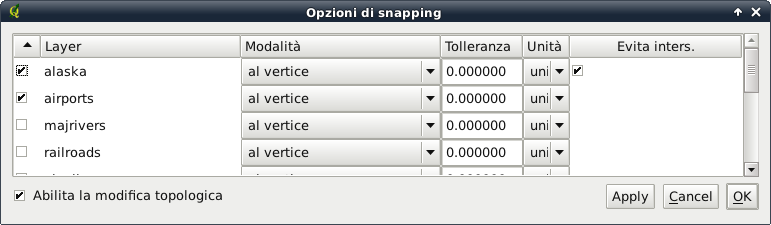
\includegraphics[clip=true, width=12cm]{editProjectSnapping}
  \caption{Édition des options d'accrochage pour chaque couche \nixcaption}\label{fig:snappingoptions}
\end{center}
\end{figure}

%\minisec{Search radius}
\minisec{Rayon de recherche}

%Search radius is the distance \qg uses to \usertext{search} for the closest vertex you are trying to move when you click on the map. If you aren't within the search radius, \qg won't find and select any vertex for editing and it will pop up an annoying warning to that effect. Snap tolerance and search radius are set in map units so you may find you need to experiment to get them set right. If you specify too big of a tolerance, \qg may snap to the wrong vertex, especially if you are dealing with a large number of vertices in close proximity. Set search radius too small and it won't find anything to move.
Le rayon de recherche est la distance que \qg utilise pour \usertext{chercher} le sommet le plus proche que vous souhaitez déplacer quand vous cliquez sur la carte. Si vous n'êtes pas dans le rayon de recherche, \qg ne trouvera ni ne sélectionnera de sommet à éditer et une fenêtre d'alerte désagréable apparaitra. La tolérance d'accrochage et le rayon de recherche sont définis dans les unités de la carte, vous allez peut-être avoir besoin d'expérimenter différentes valeurs avant de trouver la bonne. Si vous spécifiez une tolérance trop grande, \qg risque d'accrocher le mauvais sommet, surtout si vous avez un grand nombre de sommets à proximité. Définissez un rayon de recherche trop petit et \qg ne trouvera rien à déplacer.

%The search radius for vertex edits in layer units can be defined in the \tab{Digitizing} tab under \mainmenuopt{Settings} > \dropmenuopttwo{mActionOptions}{Options}. The same place where you define the general, project wide snapping tolerance.
Le rayon de recherche pour l'édition des sommets dans l'unité de la couche peut être défini dans l'onglet \tab{Numérisation} de \mainmenuopt{Préférences} > \dropmenuopttwo{mActionOptions}{Options}. Au même endroit que vous définissez la tolérance d'accrochage pour tout le projet.

% \subsection{Zooming and Panning}
\subsection{Zoomer et se déplacer}

% Before editing a layer, you should zoom in to your area of interest. This
% avoids waiting while all the vertex markers are rendered across the entire
% layer.

Avant d'éditer une couche, vous devriez zoomer sur la zone qui vous intéresse. Cela évite de devoir attendre que tous les sommets soient calculés sur l'ensemble de la couche.

% Apart from using the \toolbtntwo{mActionPan}{pan} and
% \toolbtntwo{mActionZoomIn}{zoom-in}/\toolbtntwo{mActionZoomOut}{zoom-out}
% icons on the toolbar with the mouse, navigating can also be done with the
% mouse wheel, spacebar and the arrow keys.

Au lieu d'utiliser les icones \toolbtntwo{mActionPan}{Se déplacer dans la carte} et \toolbtntwo{mActionZoomIn}{zoom +}/\toolbtntwo{mActionZoomOut}{zoom -} de la barre d'outils avec la souris, la navigation peut également se faire avec la roulette de la souris, la barre espace et les flèches du clavier.

% \minisec{Zooming and panning with the mouse wheel}
\minisec{Zoomer et bouger avec la souris}

% While digitizing you can press the mouse wheel to pan inside of the main
% window and you can roll the mouse wheel to zoom in and out on the map. For
% zooming place the mouse cursor inside the map area and roll it forward (away
% from you) to zoom in and backwards (towards you) to zoom out. The mouse cursor position
% will be the center of the zoomed area of interest. You can customize the behavior
% of the mouse wheel zoom using the \tab{Map tools} tab under the
% \mainmenuopt{Settings} >\dropmenuopt{Options} menu.

Lorsque vous numérisez vous pouvez appuyer sur la roulette de la souris pour vous déplacer dans la fenêtre principale et la faire rouler pour zoomer la carte. Pour vous rapprocher, faites rouler la molette vers l'avant tandis que si vous voulez vous éloigner vous devrez la faire rouler vers vous. La position du curseur sera le centre la zone affichée. Vous pouvez personnaliser le zoom en utilisant l'onglet \tab{Outils cartographiques} dans le menu \mainmenuopt{Préférences} >\dropmenuopt{Options}.

% \minisec{Panning with the arrow keys}
\minisec{Se déplacer avec les touches du clavier}

% Panning the Map during digitizing is possible with the arrow keys. Place
% the mouse cursor inside the map area and click on the right arrow key to
% pan east, left arrow key to pan west, up arrow key to pan north and down
% arrow key to pan south.

Il est possible de se déplacer sur la carte en utilisant les flèches du clavier. Placez votre curseur sur la carte et appuyez sur la flèche de droite pour vous déplacer vers l'Est, la flèche de gauche pour aller à l'Ouest, la flèche du haut pour le Nord et celle du bas pour le Sud.

% You can also use the spacebar to temporarily cause mouse movements to pan
% then map. The PgUp and PgDown keys on your keyboard will cause the map
% display to zoom in or out without interrupting your digitising session.

Vous pouvez utiliser la barre d'espace pour que les mouvements de la souris se traduisent par un déplacement sur la carte. Les touches PgUp et PgDown vous permettront de zoomer sans devoir interrompre votre numérisation.

%\subsection{Topological editing}
\subsection{Édition topologique}

%Besides layer based snapping options the \tab{General} tab in menu \mainmenuopt{Settings} -> \dropmenuopttwo{mActionOptions}{Project Properties\dots} also provides some topological functionalities. In the Digitizing option group you can \checkbox{Enable topological editing} and/or activate \checkbox{Avoid intersections of new polygons}.
En plus des options d'accrochage pour chaque couche, l'onglet \tab{Général} du menu\\ \mainmenuopt{Préférences} > \dropmenuopttwo{mActionOptions}{Propriétés du projet\dots} propose quelques fonctionnalités topologiques. Dans le groupe d'options de Numérisation, vous pouvez \checkbox{Activer l'édition topologique} et/ou activer\\ \checkbox{Éviter les intersections de nouveaux polygones}.

%\minisec{Enable topological editing}
\minisec{Activer l'édition topologique}

%The option \checkbox{Enable topological editing} is for editing and maintaining common boundaries in polygon mosaics. \qg "detects" a shared boundary in a polygon mosaic and you only have to move the vertex once and \qg will take care about updating the other boundary.
L'option \checkbox{Activer l'édition topologique} permet d'éditer en gardant des limites communes entre les polygones. \qg "détecte" une limite commune entre les polygones et vous avez simplement à déplacer le sommet une fois et \qg s'occupera de mettre à jour l'autre limite.

%\minisec{Avoid intersections of new polygons}
\minisec{Éviter les intersections de nouveaux polygones}

%The second topological option called \checkbox{Avoid intersections of new polygons} avoids overlaps in polygon mosaics. It is for quicker digitizing of adjacent polygons. If you already have one polygon, it is possible with this option to digitise the second one such that both intersect and qgis then cuts the second polygon to the common boundary. The advantage is that users don't have to digitize all vertices of the common boundary.
La deuxième option topologique, \checkbox{Éviter les intersections de nouveaux polygones}, permet d'éviter des recouvrements entre les polygones. Cela permet de numériser des polygones adjacents plus rapidement. Si vous avez déjà un polygone, avec cette option, vous pouvez numériser le second de manière à ce qu'ils intersectent et \qg coupera le second polygone aux limites communes. L'avantage est que les utilisateurs n'ont pas à numériser tous les sommets des limites communes.

%\subsection{Editing an Existing Layer}
\subsection{Numériser une couche existante}
\index{couches vecteur!numériser}
\index{numeriser!une couche existante}
\label{sec:edit_existing_layer}

%By default, \qg loads layers read-only: This is a safeguard to avoid accidentally editing a layer if there is a slip of the mouse. However, you can choose to edit any layer as long as the data provider supports it, and the underlying data source is writable (i.e. its files are not read-only).
Par défaut, \qg charge les couches en lecture seule : c'est une sécurité pour éviter d'éditer accidentellement une couche si la souris a glissé. Cependant, vous pouvez choisir d'éditer une couche du moment que le fournisseur de données le gère et que la source de données est éditable (c.-à-d. fichiers qui ne sont pas en lecture seule). 
%Layer editing is most versatile when used on PostgreSQL/PostGIS data sources.
L'édition d'une couche est plus flexible lorsqu'il s'agit de sources de données PostgreSQL/PostGIS.

% In general, editing vector layers is divided into a digitizing and an advanced
% digitizing toolbar, described in Section \ref{sec:advanced_edit}. You can
% select and unselect both under \mainmenuopt{Settings} > \dropmenuopt{Toolbars}.
% Using the basic digitizing tools you can perform the following functions:

En général, l'édition des couches vecteurs est répartie dans une barre de numérisation et une barre de numérisation avancée telle que décrite dans la section \ref{sec:advanced_edit}. Vous pouvez sélectionner les deux dans \mainmenuopt{Préférences} > \dropmenuopt{Barre d'Outils}. En utilisant les outils basiques de numérisation, vous pouvez accomplir les actions suivantes :

%\begin{Tip}[ht]\caption{\textsc{Data Integrity}}
\begin{Tip}[ht]\caption{\textsc{Intégrité des données}}
%\qgistip{It is always a good idea to back up your data source before you start editing. While the authors of \qg have made every effort to preserve the integrity of your data, we offer no warranty in this regard.}
Sauvegarder vos données avant de se lancer dans une édition est toujours une bonne idée. Bien que les auteurs de \qg ont fait beaucoup d'efforts pour préserver l'intégrité de vos données, nous n'offrons aucune garantie.
\end{Tip}
%traduction
\begin{table}[ht]\index{vector layers!basic editing tools}
\centering

\begin{tabular}{|l|p{5.5cm}|l|p{5.5cm}|}
\hline \textbf{Icon} & \textbf{Purpose} & \textbf{Icon} & \textbf{Purpose} \\
\hline 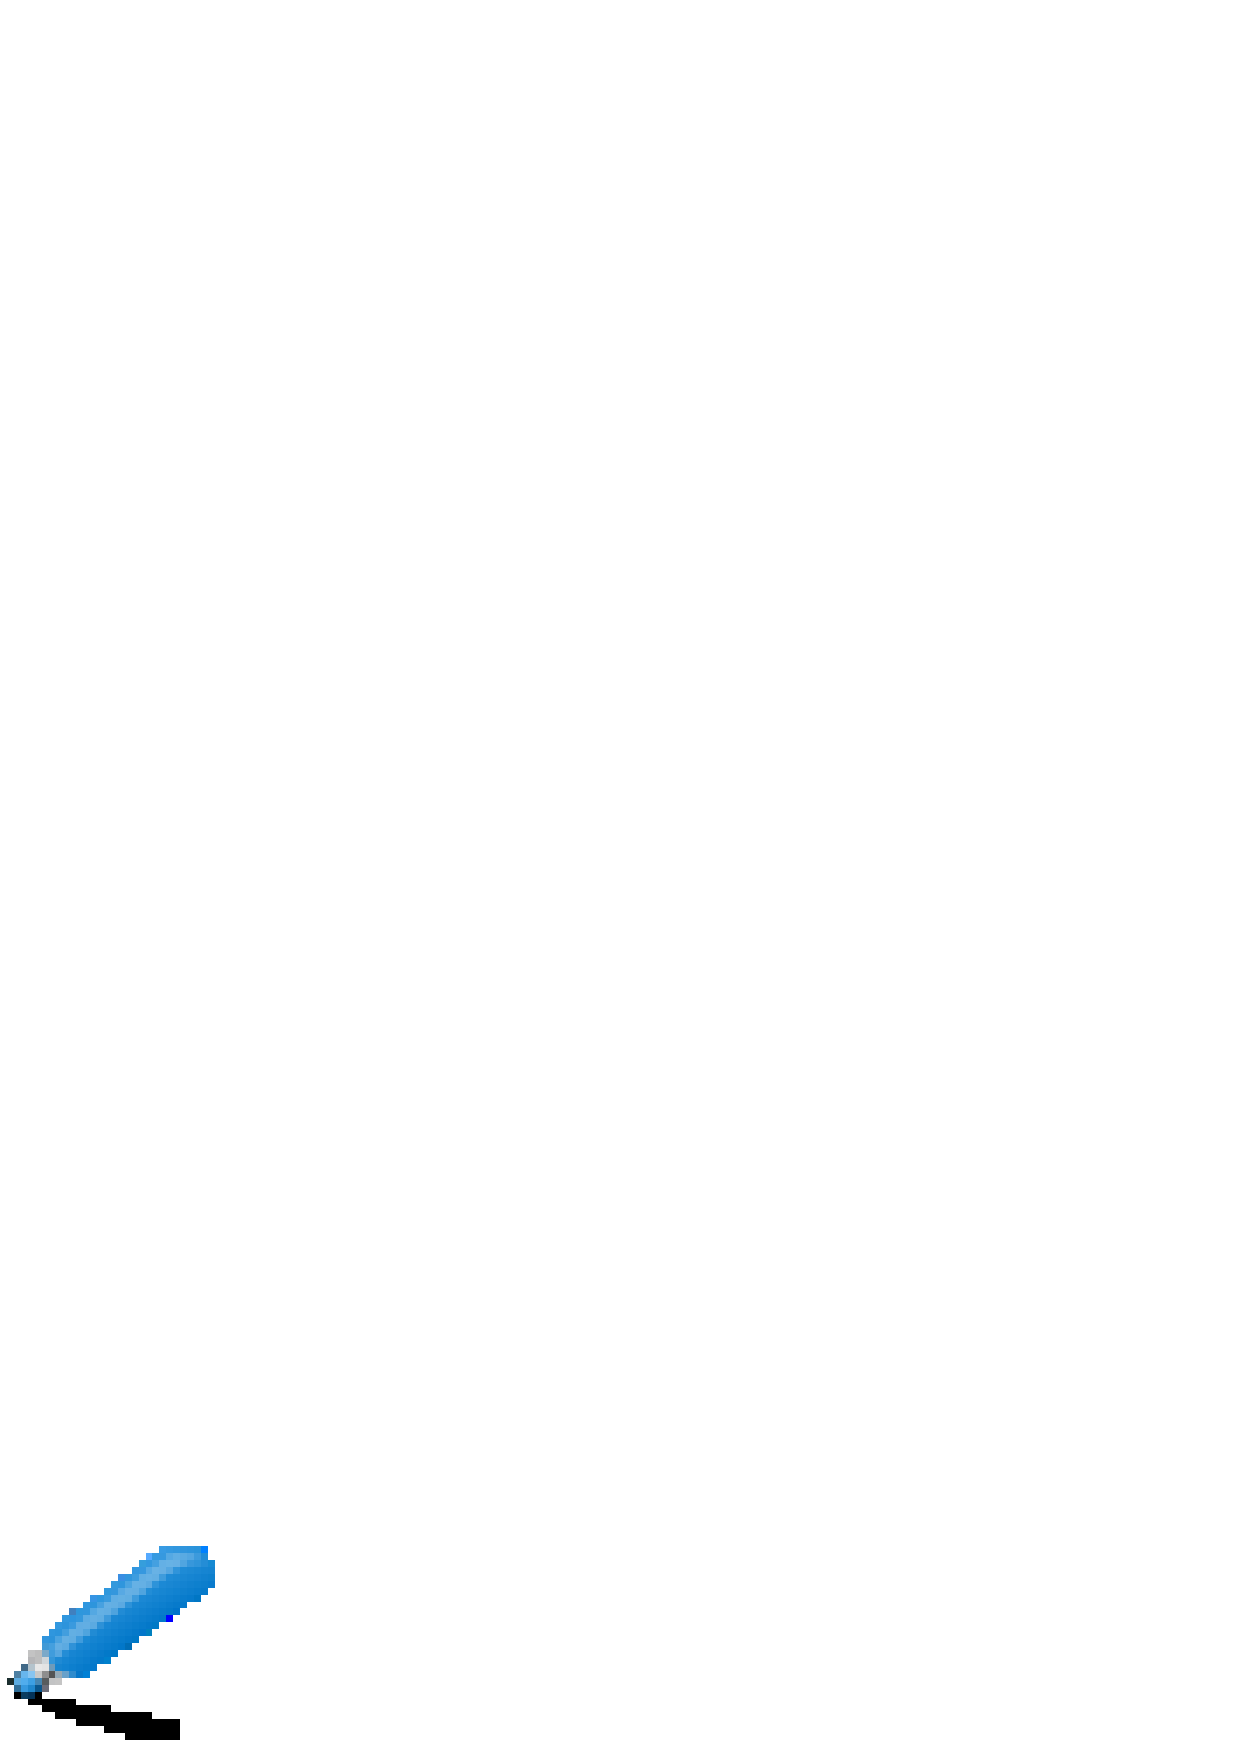
\includegraphics[width=0.7cm]{mActionToggleEditing}
   & Basculer en mode édition
   & 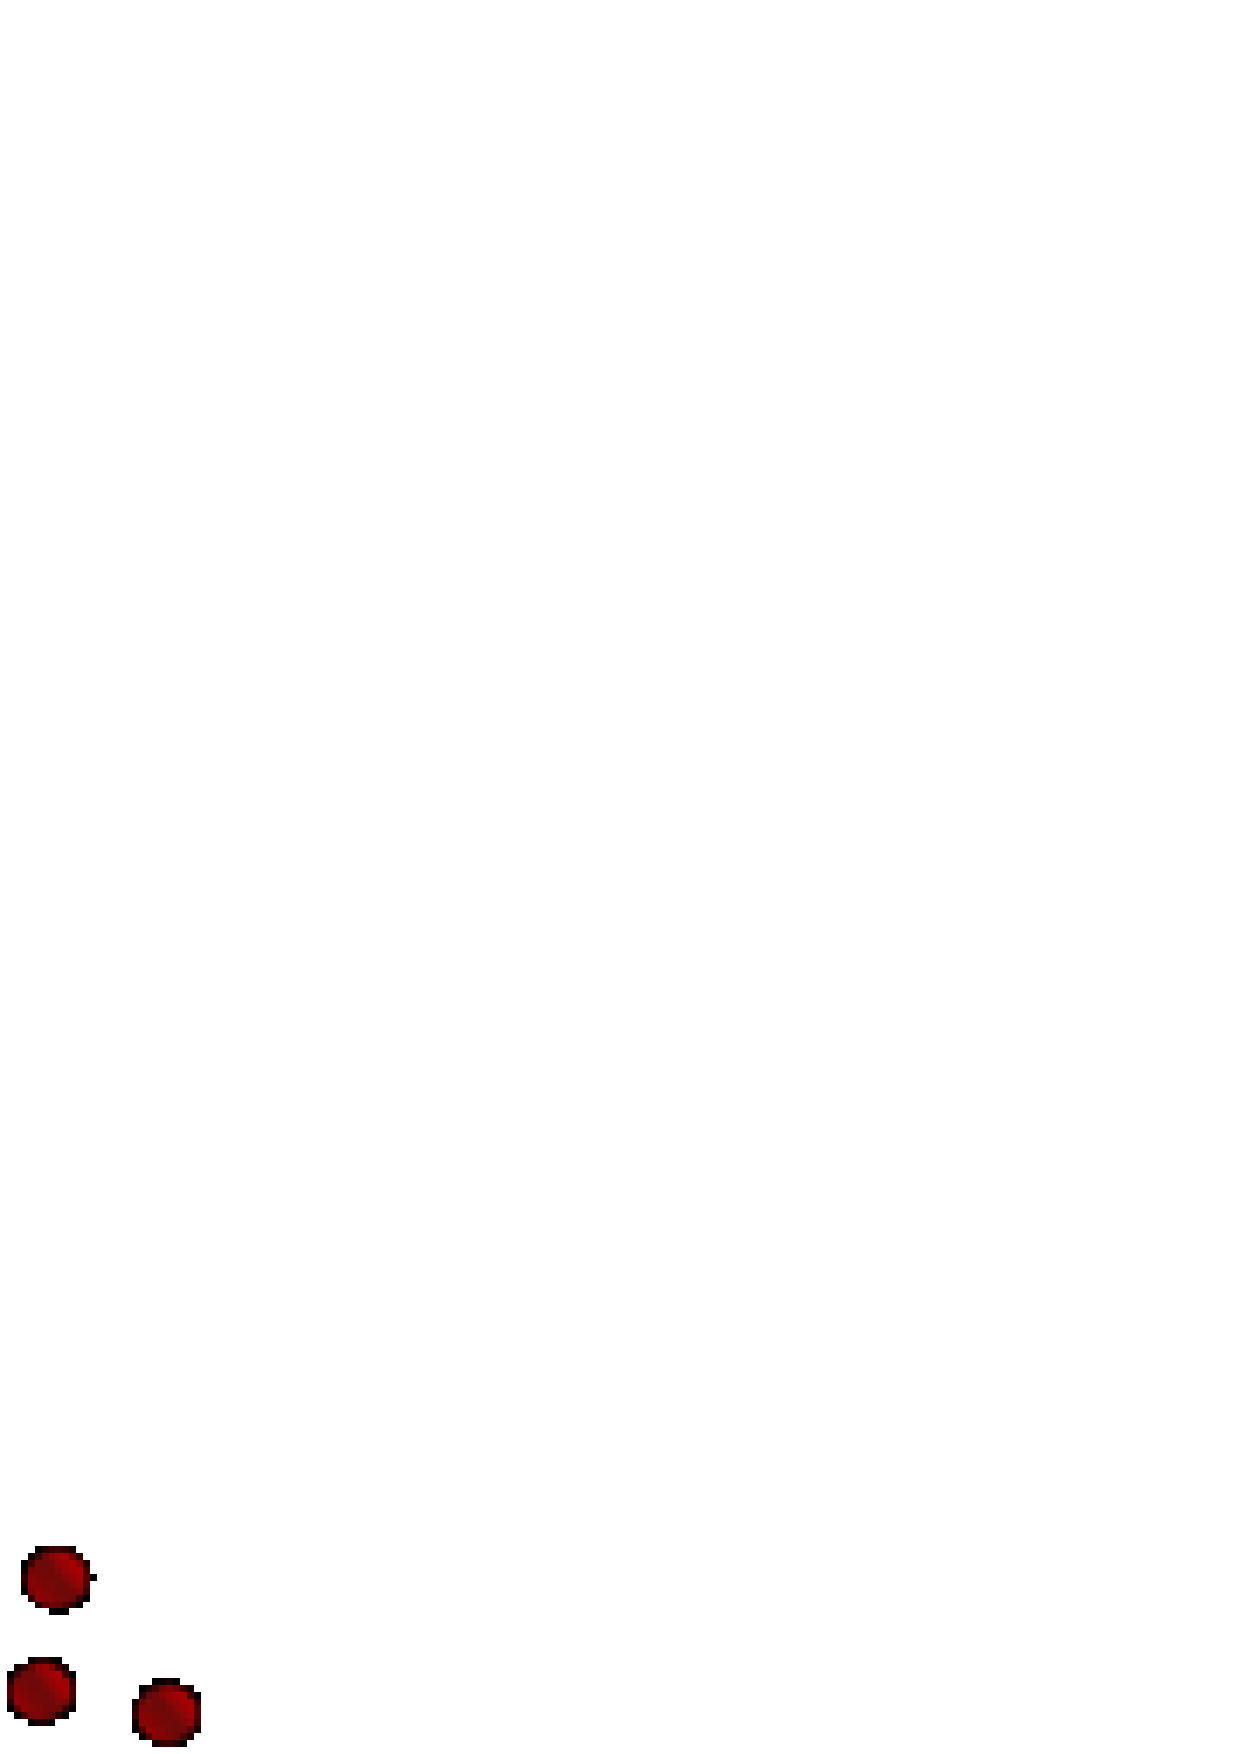
\includegraphics[width=0.7cm]{mActionCapturePoint}
   & Ajouter une entité: Créer un point \\
\hline 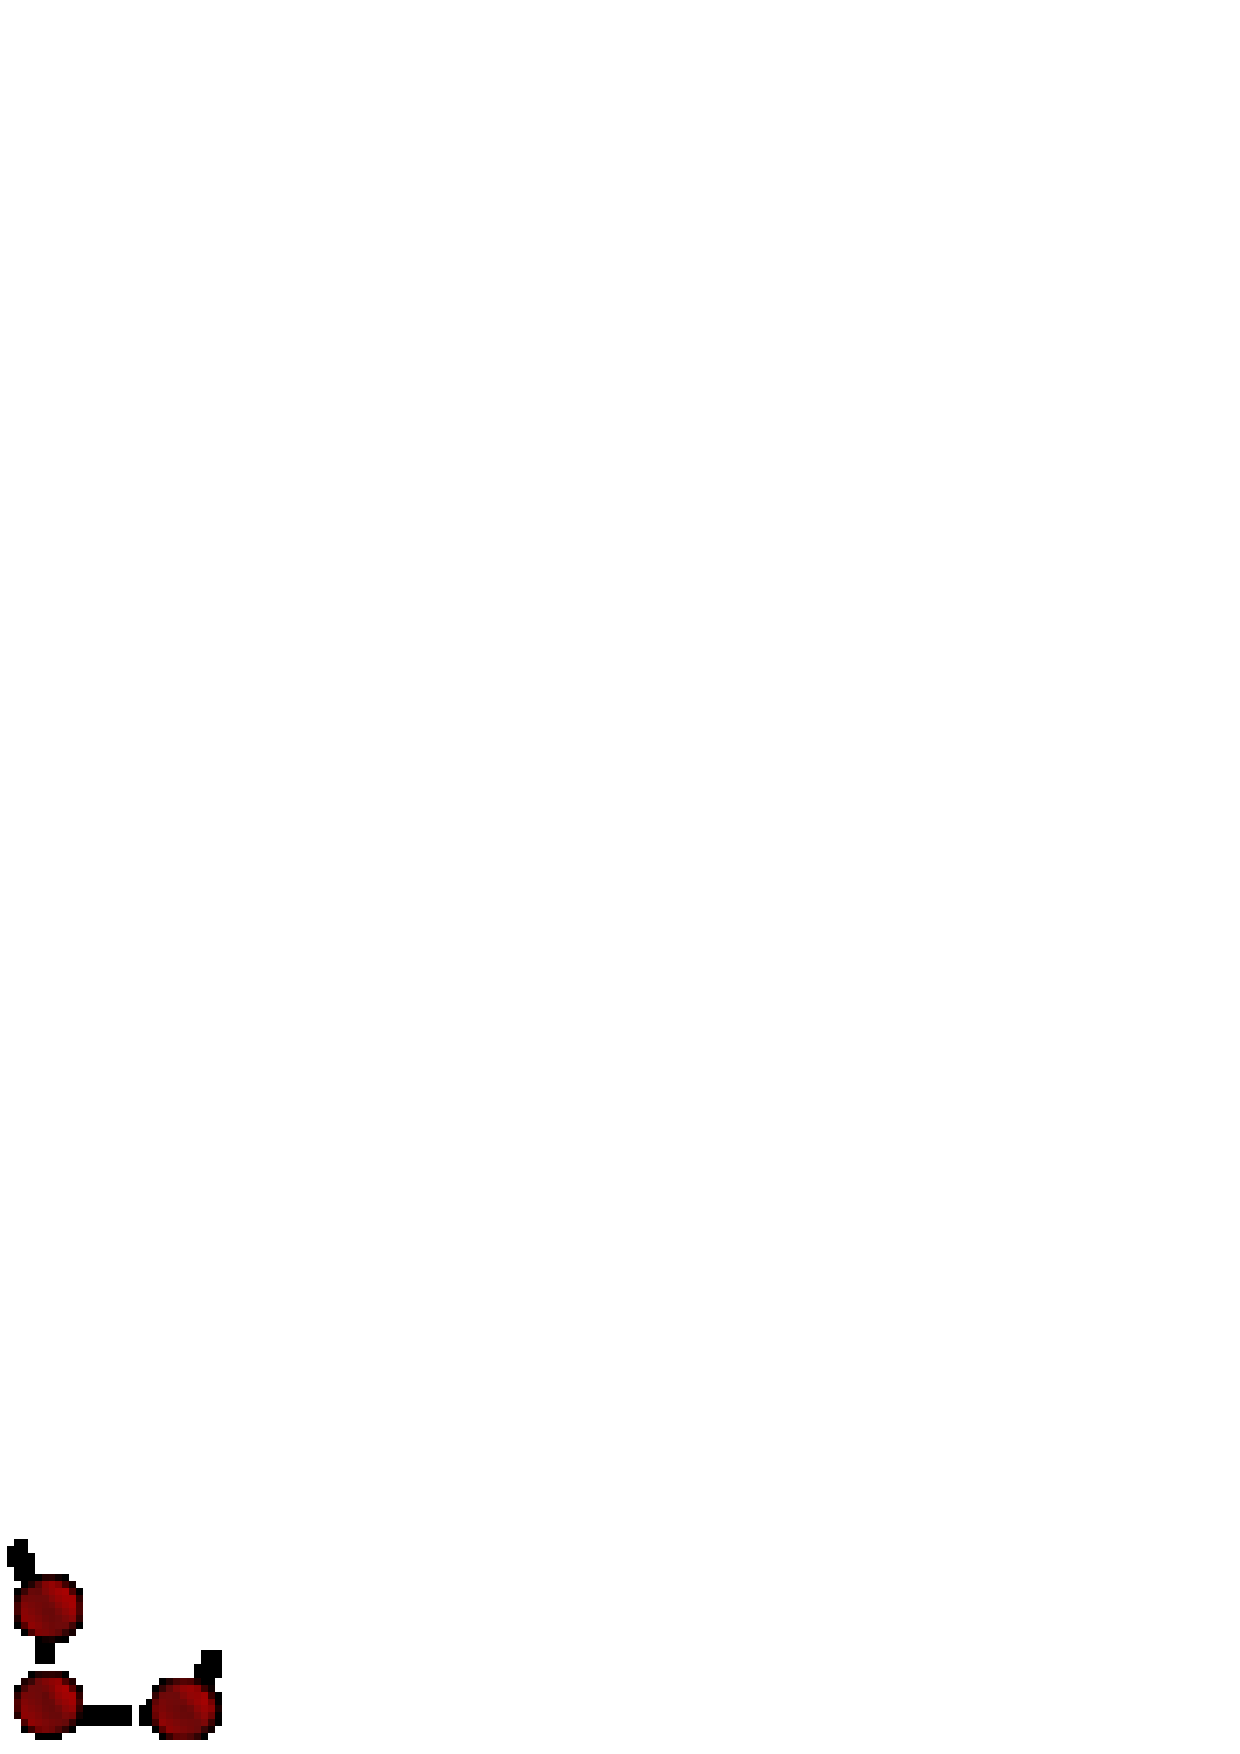
\includegraphics[width=0.7cm]{mActionCaptureLine}
   & Ajouter une entité: Créer une Ligne
   & 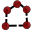
\includegraphics[width=0.7cm]{mActionCapturePolygon}
   & Ajouter une entité: Créer un polygone \\
\hline 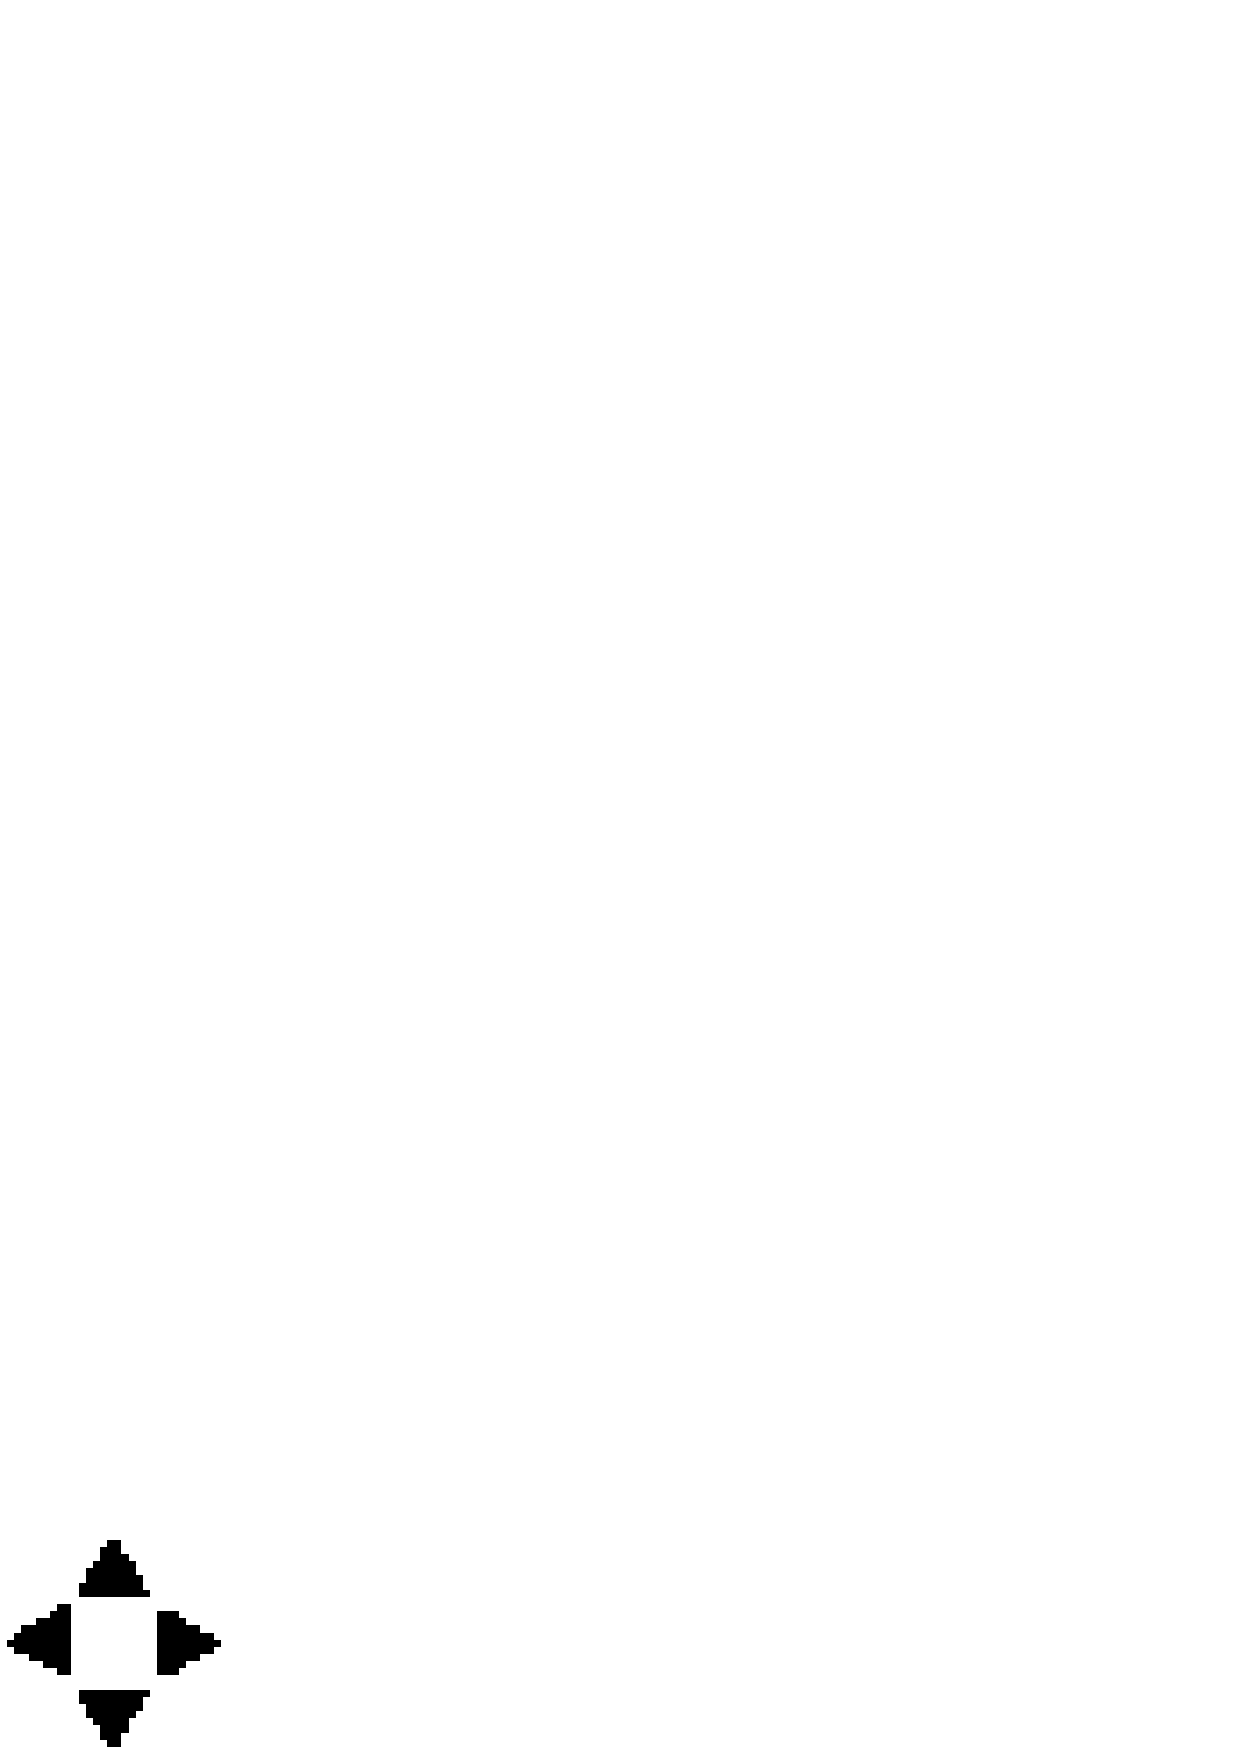
\includegraphics[width=0.7cm]{mActionMoveFeature}
   & Déplacer une entité
   & 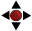
\includegraphics[width=0.7cm]{mActionMoveVertex}
   & Déplacer un sommet\\
\hline 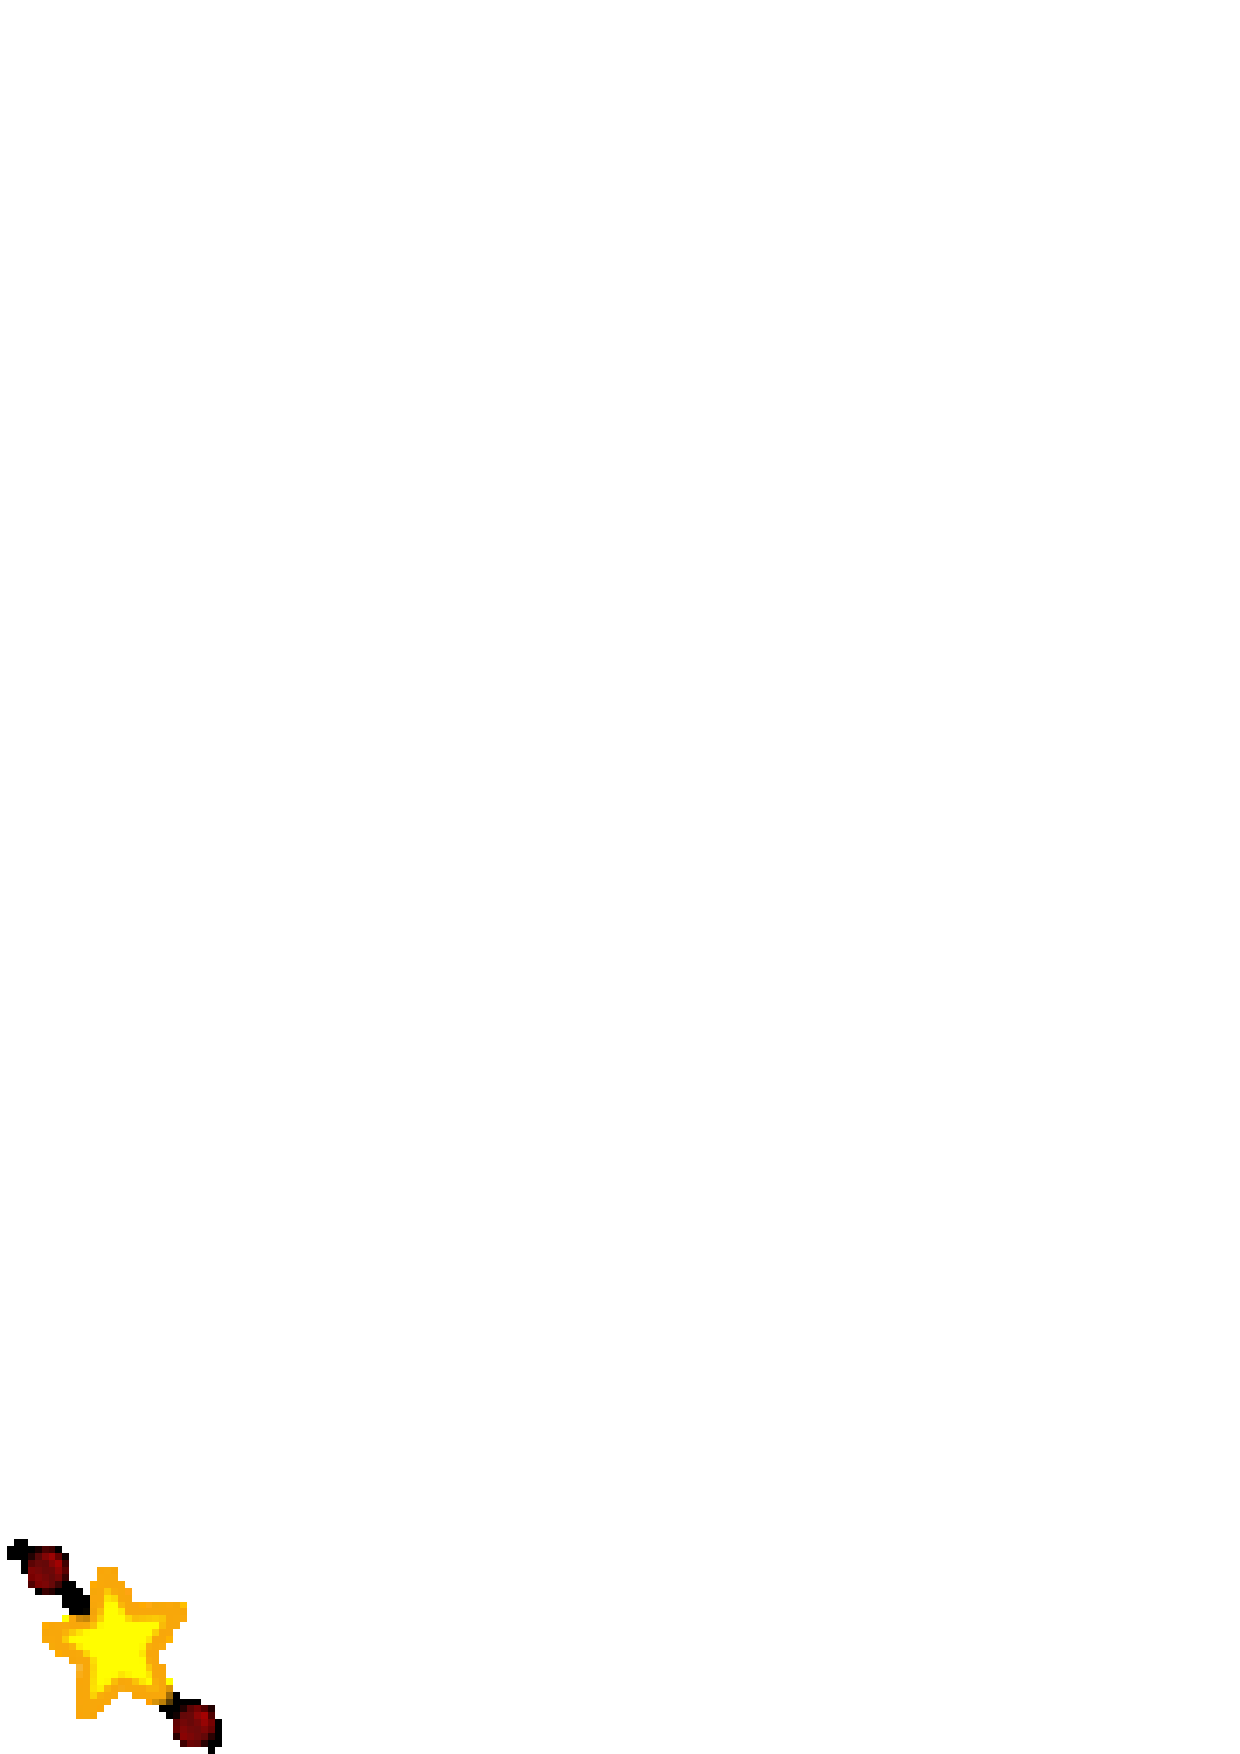
\includegraphics[width=0.7cm]{mActionAddVertex}
   & Ajouter un sommet
   & 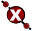
\includegraphics[width=0.7cm]{mActionDeleteVertex}
   & Effacer un sommet \\
\hline 
\includegraphics[width=0.7cm]{mActionDeleteSelected}
   & Effacer la sélection
   & 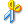
\includegraphics[width=0.7cm]{mActionEditCut}
   & Couper une entité \\
\hline 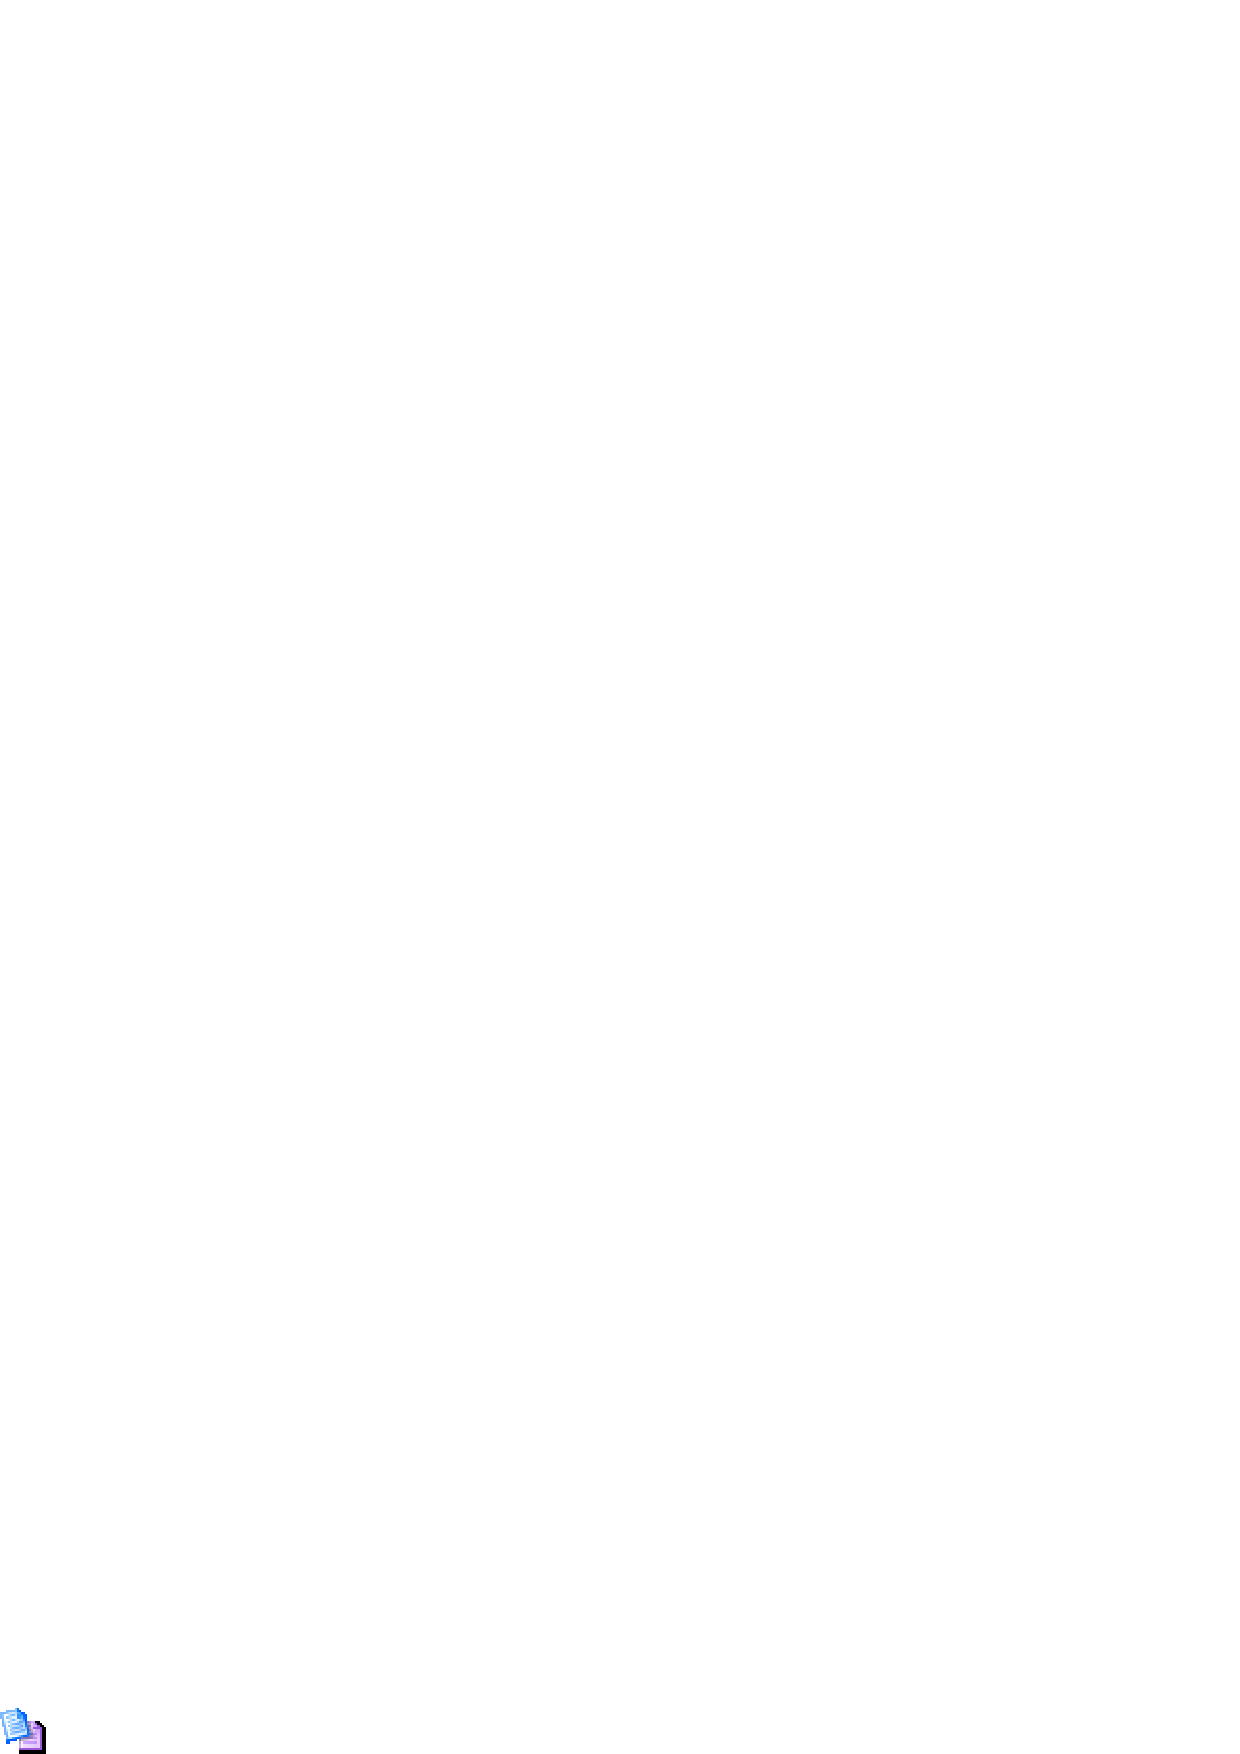
\includegraphics[width=0.7cm]{mActionEditCopy}
   & Copier une entité 
   & 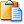
\includegraphics[width=0.7cm]{mActionEditPaste} 
   & Coller une entité \\
\hline
\end{tabular}
\caption{Vector layer basic editing toolbar}\label{tab:vector_editing}
\end{table}

% All editing sessions start by choosing the
% \dropmenuopttwo{mActionToggleEditing}{Toggle editing} option.
% This can be found in the context menu after right clicking on the legend
% entry for that layer.\index{Allow Editing}

Toutes les sessions d'édition débutent par la sélection de l'option\\ \dropmenuopttwo{mActionToggleEditing}{Basculer en mode édition}. Elle se trouve dans le menu contextuel après un clic droit sur la couche voulue.

% Alternately, you can use the \index{Toggle Editing}
% \toolbtntwo{mActionToggleEditing}{Toggle editing} button from the digitizing
% toolbar to start or stop the editing mode.\index{editing!icons} Once the
% layer is in edit mode, markers will appear at the vertices, and additional
% tool buttons on the editing toolbar will become available.

Alternativement, vous pouvez utiliser le bouton \index{Basculer en mode édition}\toolbtntwo{mActionToggleEditing}{Basculer en mode édition} dans la barre de numérisation pour débuter ou terminer une session d'édition.\index{numerisation!icones} Une fois que la couche est éditable, les marqueurs vont apparaître sur les sommets et de nouveaux outils seront disponibles dans la barre d'outils.

%\begin{Tip}[ht]\caption{\textsc{Save Regularly}}
\begin{Tip}[ht]\caption{\textsc{Fréquence de sauvegarde}}
%\qgistip{Remember to toggle \toolbtntwo{mActionToggleEditing}{Toggle editing} off regularly. This allows you to save your recent changes, and also confirms that your data source can accept all your changes.}
N'oubliez pas de cliquer sur \toolbtntwo{mActionToggleEditing}{Basculer en mode édition} régulièrement. Cela vous permet de sauvegarder les changements récents, mais également de confirmer que votre source de données accepte tous vos changements.
\end{Tip}

%All editing sessions start by choosing the \dropmenuopttwo{mActionToggleEditing}{Toggle editing} option. This can be found in the context menu after right clicking on the legend entry for that layer.\index{Allow Editing} Alternately, you can use the \index{Toggle Editing} \toolbtntwo{mActionToggleEditing}{Toggle editing} button from the toolbar to start or stop the editing mode.\index{editing!icons} Once the layer is in edit mode, markers will appear at the vertices, and additional tool buttons on the editing toolbar will become available.
Toute session d'édition commence par un clic sur \dropmenuopttwo{mActionToggleEditing}{Basculer en mode édition}. Ceci se trouve dans le menu contextuel qui apparaît après un clic droit sur la couche dans la légende.\index{Autoriser l'édition} Sinon, vous pouvez utiliser le bouton \index{Basculer en mode édition} \toolbtntwo{mActionToggleEditing}{Basculer en mode édition} de la barre d'outils pour lancer ou stopper l'édition. \index{éditer!icônes} Une fois la couche en mode édition, les marqueurs apparaissent sur les sommets et de nouveaux outils de la barre d'outils édition sont disponibles.

%\minisec{Adding Features}
%\index{vector layers!adding!feature}
\minisec{Ajouter et déplacer des entités}
\index{couches vecteur!déplacer!entités}

%Before you start adding features, use the \toolbtntwo{mActionPan}{pan} and \toolbtntwo{mActionZoomIn}{zoom-in}/\toolbtntwo{mActionZoomOut}{zoom-out} tools to first navigate to the area of interest.
Avant de commencer à ajouter des entités, utiliser les outils \toolbtntwo{mActionPan}{Se déplacer dans la carte} et \toolbtntwo{mActionZoomIn}{zoom +}/\toolbtntwo{mActionZoomOut}{zoom -} pour naviguer vers la zone d'intérêt.

%Then you can use the \toolbtntwo{mActionCapturePoint}{Capture point}, \toolbtntwo{mActionCaptureLine}{Capture line} or \toolbtntwo{mActionCapturePolygon}{Capture polygon} icons on the toolbar to put the \qg cursor into digitizing mode.
Vous pouvez utiliser \toolbtntwo{mActionCapturePoint}{Capturer le Point}, \toolbtntwo{mActionCaptureLine}{Capturer la Ligne} ou\\ \toolbtntwo{mActionCapturePolygon}{Capturer le Polygone} dans la barre d'outils pour mettre le curseur de \qg en mode numérisation.

%For each feature, you first digitize the geometry, then enter its attributes.
Pour chaque entité, vous numérisez d'abord la géométrie puis entrez les attributs.

%To digitize the geometry, left-click on the map area to create the first point of your new feature.
Pour numériser la géométrie, faites un clic gauche sur la zone de la carte pour créer le premier point de votre nouvelle entité.

%For lines and polygons, keep on left-clicking for each additional point you wish to capture.  When you have finished adding points, right-click anywhere on the map area to confirm you have finished entering the geometry of that feature.
Pour les lignes ou les polygones, continuer à faire des clics gauches pour chaque nouveau point que vous souhaitez capturer. Lorsque vous avez fini d'ajouter des points, faites un clic droit n'importe où sur la carte pour confirmer que vous avez fini d'entrer la géométrie de cette entité.

%The attribute window will appear, allowing you to enter the information for the new feature. Figure \ref{fig:vector_digitising} shows setting attributes for a fictitious new river in Alaska.
La fenêtre des attributs apparaît, ce qui vous permet d'entrer les informations sur la nouvelle entité. La figure \ref{fig:vector_digitising} montre les attributs d'édition pour une nouvelle rivière fictive en Alaska.

\begin{figure}[ht]
  \begin{center}
  %\caption{Enter Attribute Values Dialog after digitizing a new vector feature \nixcaption}\label{fig:vector_digitising}\smallskip
 
  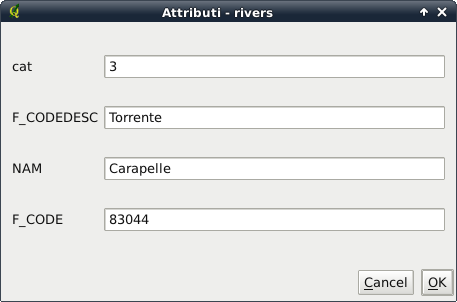
\includegraphics[clip=true, width=8cm]{editDigitizing}
  \caption{Fenêtre Entrez les valeurs d'attributs après la numérisation d'une nouvelle entité vecteur \nixcaption}\label{fig:vector_digitising}
\end{center}
\end{figure}

Avec l'icône \toolbtntwo{mActionMoveFeature}{Déplacer Entités}, vous pouvez déplacer des entités existantes.

%\begin{Tip}[ht]\caption{\textsc{Attribute Value Types}}
\begin{Tip}[ht]\caption{\textsc{Types des valeurs d'attribut}}
%\qgistip{At least for shapefile editing the attribue types are validated during the entry. Because of this, it is not possible to enter a number into the text-column in the dialog \dialog{Enter Attribute Values} or vica versa. If you need to do so, you should edit the attributes in a second step within the \dialog{Attribute table} dialog.}
Pour l'édition des shapefiles au moins, les types des attributs sont validés au moment de la saisie. À cause de cela, il n'est pas possible d'entrer un nombre dans un champ de type texte dans la fenêtre \dialog{Entrez les valeurs d'attributs} et vice-versa. Si vous avez besoin de le faire, vous devez éditer les attributs par la suite dans la fenêtre \dialog{Table d'attributs}.
\end{Tip}

%\minisec{Editing Vertices of a Feature}
%\index{vector layers!editing!vertex}
\minisec{Ajouter, déplacer et éditer les sommets d'un objet}
\index{couches vecteur!éditer!objet}

%For both PostgreSQL/PostGIS and shapefile-based layers, the vertices of features can be edited.
Pour les couches PostgreSQL/PostGIS et shapefile, on peut éditer les sommets des entités.

%Vertices can be directly edited, that is, you don't have to choose which feature to edit before you can change its geometry. In some cases, several features may share the same vertex and so the following rules apply when the mouse is pressed down near map features:
Les sommets peuvent être édités directement, ce qui signifie que vous n'avez pas à choisir quelle entité vous voulez éditer avant que vous puissiez changer sa géométrie. Dans certains cas, plusieurs entités peuvent partager le même sommet et voilà les règles qui s'appliquent lorsqu'un bouton de la souris est pressé proche d'une entité :

\begin{description}
%\item \textbf{Lines}    - The nearest line to the mouse position is used as the target feature. Then (for moving and deleting a vertex) the nearest vertex on that line is the editing target.
\item[Lignes :] La ligne la plus proche de la position de la souris est utilisée comme entité cible. Ensuite (pour déplacer ou supprimer un sommet) le sommet le plus proche sur cette ligne est la cible de l'édition.
%\item \textbf{Polygons} - If the mouse is inside a polygon, then it is the target feature; otherwise the nearest polygon is used. Then (for moving and deleting a vertex) the nearest vertex on that polygon is the editing target.
\item[Polygones :] Si la souris est à l'intérieur d'un polygone, celui-ci est l'entité ciblée ; autrement, le polygone le plus proche est utilisé. Ensuite (pour déplacer ou supprimer un sommet) le sommet le plus proche sur ce polygone est la cible de l'édition.
\end{description}

%You will need to set the property \mainmenuopt{Settings}>\dropmenuopttwo{mActionOptions}{Options}>\tab{Digitizing}>\selectnumber{Search Radius}{10} to a number greater than zero.  Otherwise \qg will not be able to tell which feature is being edited.
Vous aurez à définir le paramètre\\ \mainmenuopt{Préférences}>\dropmenuopttwo{mActionOptions}{Options}>\tab{Numérisation}>\selectnumber{Rayon de recherche}{10} à un nombre supérieur à zéro. Sinon \qg ne sera pas en mesure de dire quelle entité est éditée.

%You can add new vertices to a feature by using the \toolbtntwo{mActionAddVertex}{Add Vertex} icon on the toolbar.
Vous pouvez ajouter de nouveaux sommets à une entité en utilisant le bouton\\ \toolbtntwo{mActionAddVertex}{Ajouter un Sommet} de la barre d'outils. Notez qu'il n'y a aucun sens à ajouter des sommets à des entités de type ponctuelles !

% \begin{Tip}[ht]\caption{\textsc{Vertex Markers}}
% \qgistip{The current version of \qg supports two kinds of vertex-markers -
% a semi-transparent circle or a cross. To change the marker style, choose
% \dropmenuopttwo{mActionOptions}{Options} from the \mainmenuopt{Settings} menu
% and click on the \tab{Digitizing} tab and select the appropriate entry.
% }
% \end{Tip}

\begin{Tip}[ht]\caption{\textsc{Marqueurs de sommets}}
La version actuelle de \qg présente 2 types de marqueurs - un cercle semi-transparent ou une croix. Pour changer de style de marqueurs, allez dans le menu \dropmenuopttwo{mActionOptions}{Options} et cliquez sur l'onget \tab{Numérisation} et sélectionnez le symbole voulu dans la liste déroulante.
\end{Tip}

%In this version of \qg, vertices can only be added to an \textit{existing} line segment of a line feature.  If you want to extend a line beyond its end, you will need to move the terminating vertex first, then add a new vertex where the terminus used to be.
Dans cette version de \qg, les sommets peuvent uniquement être ajoutés à un segment de ligne \textit{existant}. Si vous voulez étendre une ligne au-delà de ses extrémités, vous devez d'abord déplacer le sommet terminal puis ajouter un nouveau sommet là où le sommet terminal était.

%You can move vertices using the \toolbtntwo{mActionMoveVertex}{Move Vertex} icon on the toolbar.
Vous pouvez déplacer des sommets en utilisant le bouton \toolbtntwo{mActionMoveVertex}{Déplacer le Sommet} de la barre d'outils.

% With the \toolbtntwo{mActionDeleteVertex}{Delete Vertex} icon on the toolbar
% you can delete vertices.\index{vector layers!deleting!vertex} Please note, it
% doesn't make sense to delete the vertex of a Point feature! Delete the whole
% feature instead.

Avec le bouton \toolbtntwo{mActionDeleteVertex}{Effacer un Sommet} vous pouvez supprimer des sommets.\index{vector layers!deleting!vertex}. Notez qu'il n'y a pas de sens à supprimer un sommet d'une entité ponctuelle ! Supprimer l'entité complète à la place.

%Similarly, a one-vertex line or a two-vertex polygon is also fairly useless and will lead to unpredictable results elsewhere in \qg, so don't do that.
De la même manière, une ligne avec un seul sommet ou un polygone à deux sommets n'ont pas d'intérêt et entraîneraient des comportements imprévisibles dans \qg, donc à éviter. 

%\textbf{Warning:} A vertex is identified for deletion as soon as you click the mouse near an eligible feature. To undo, you will need to toggle Editing off and then discard your changes. (Of course this will mean that other unsaved changes will be lost, too.)
\textbf{Attention :} Un sommet est identifié pour la suppression dès que vous cliquer à proximité d'une entité. Pour annuler cela, vous devez sortir du mode édition sans sauvegarder vos changements. (Bien entendu cela signifie que tous les changements non sauvegardés seront perdus).

%\minisec{Add Ring}
%\index{vector layers!add!ring}
\minisec{Ajouter un anneau}
\index{couches vecteur!ajouter!anneau}

%You can create ring polygons using the \toolbtntwo{mActionAddRing}{Add Ring} icon in the toolbar. This means inside an existing area it is possible to digitize further polygons, that will occur as a 'whole', so only the area in between the boundaries of the outer and inner polygons remain as a ring polygon.
Vous pouvez créez des polygones de type anneau en utilisant le bouton \toolbtntwo{mActionAddRing}{Ajouter Anneau} de la barre d'outils. Ceci signifie qu'il est possible de numériser des polygones à l'intérieur d'une entité existante, qui seront alors des 'trous' de sorte que seule la zone entre les limites externes et internes du polygone reste, créant un polygone anneau.

%\minisec{Add Island}
%\index{vector layers!add!island}
\minisec{Ajouter une île}
\index{couches vecteur!ajouter!île}

%You can \toolbtntwo{mActionAddIsland}{add island} polygons to a selected multipolygon. The new island polygon has to be digitized outside the selected multipolygon.
Vous pouvez \toolbtntwo{mActionAddIsland}{Ajouter une île} à un multipolygone sélectionné. Le nouveau polygone île soit être numérisé en dehors du multipolygone sélectionné.

%\minisec{Cutting, Copying and Pasting Features}
%\index{vector layers!cut!feature}
%\index{vector layers!copy!feature}
%\index{vector layers!paste!feature}
%\index{editing!cutting features}
%\index{editing!copying features}
%\index{editing!pasting features}
\minisec{Couper, Copier et Coller des entités}
\index{couches vecteur!couper!entité}
\index{couches vecteur!copier!entité}
\index{couches vecteur!coller!entité}
\index{éditer!couper des entités}
\index{éditer!copier des entités}
\index{éditer!coller des entités}

%Selected features can be cut, copied and pasted between layers in the same \qg project, as long as destination layers are set to  \toolbtntwo{mActionToggleEditing}{Toggle editing} beforehand.
Une entité sélectionnée peut être coupée, copiée et collée entre des couches d'un même projet \qg, du moment que les couches de destination sont \toolbtntwo{mActionToggleEditing}{Basculées en mode édition} au préalable.

%Features can also be pasted to external applications as text:  That is, the features are represented in CSV format with the geometry data appearing in the OGC Well-Known Text (WKT) format.
Les entités peuvent également être collées dans des applications externes au format texte. Les entités sont alors représentées au format CSV et leur géométrie apparaît dans le format OGC Well-Known Text (WKT).

%However in this version of \qg, text features from outside \qg cannot  be pasted to a layer within \qg. When would the copy and paste function come in handy? Well, it turns out that you can edit more than one layer at a time and copy/paste features between layers. Why would we want to do this?  Say we need to do some work on a new layer but only need one or two lakes, not the 5,000 on our \filename{big\_lakes} layer. We can create a new layer and use copy/paste to plop the needed lakes into it.
Cependant, dans cette version de \qg, les entités au format texte venant d'applications externes ne peuvent pas être collées à une couche dans \qg. En quoi les fonctions copier et coller sont-elles utiles ? Et bien il se trouve que vous pouvez éditer plus d'une couche à la fois et que vous pouvez alors utiliser les fonctions copier/coller entre les couches. Pourquoi voudrions-nous faire cela ? Imaginons que nous devions travailler sur une nouvelle couche, mais que nous avions besoin que d'un ou deux lacs, pas les 5 000 de notre couche \filename{big\_lakes}. Nous pouvons créer une nouvelle couche puis utiliser copier/coller pour y insérer les quelques lacs.

%As an example we are copying some lakes to a new layer:
Voici un exemple de copie de quelques lacs dans une nouvelle couche :

\begin{enumerate}
%\item Load the layer you want to copy from (source layer)
\item Chargez la couche dont vous voulez copier des entités (couche source)
%\item Load or create the layer you want to copy to (target layer)
\item Chargez ou créez la couche sur laquelle vous voulez coller des entités (couche cible)
%\item Start editing for target layer
\item Lancez l'édition pour la couche cible
%\item Make the source layer active by clicking on it in the legend
\item Assurez-vous que la couche source est active en cliquant dessus dans la légende
%\item Use the \toolbtntwo{mActionSelect}{Select} tool to select the feature(s) on the source layer
\item Utilisez l'outil \toolbtntwo{mActionSelect}{Sélection} pour sélectionner les entités dans la couche source
%\item Click on the \toolbtntwo{mActionEditCopy}{Copy Features} tool
\item Cliquez sur l'outil \toolbtntwo{mActionEditCopy}{Copier Entités}
%\item Make the destination layer active by clicking on it in the legend
\item Assurez-vous que la couche cible est active en cliquant dessus dans la légende
%\item Click on the \toolbtntwo{mActionEditPaste}{Paste Features} tool
\item Cliquez sur l'outil \toolbtntwo{mActionEditPaste}{Coller Entités}
%\item Stop editing and save the changes
\item Stoppez l'édition et sauvegardez les changements
\end{enumerate}

%What happens if the source and target layers have different schemas (field names and types are not the same)? \qg populates what matches and ignores the rest. If you don't care about the attributes being copied to the target layer, it doesn't matter how you design the fields and data types. If you want to make sure everything - feature and its attributes - gets copied, make sure the schemas match.
Qu'arrive-t-il si les couches sources et cibles ont différents schémas de données (noms et type des champs différents) ? \qg remplit ceux qui correspondent et ignore les autres. Si la copie des attributs ne vous intéresse pas, la façon dont vous designer les champs et les types de données n'a pas d'importance. Si vous voulez être sûr que tout - entité et ses attributs - est copié, assurez-vous que les schémas de données correspondent.

%\begin{Tip}[ht]\caption{\textsc{Congruency of Pasted Features}}
\begin{Tip}[ht]\caption{\textsc{Congruence des entités copiées}}
%\qgistip{If your source and destination layers use the same projection, then the pasted features will have geometry identical to the source layer. However if the destination layer is a different projection then \qg cannot guarantee the geometry is identical. This is simply because there are small rounding-off errors involved when converting between projections.}
Si vos couches source et cible utilisent la même projection, les entités collées auront la même géométrie que dans la couche source. Cependant, si la couche cible n'a pas la même projection, \qg ne peut garantir que les géométries seront identiques. Cela est simplement dû aux erreurs d'arrondissement faites lors de la conversion de projection.
\end{Tip}

%\minisec{Deleting Selected Features}
%\index{vector layers!deleting!feature}
\minisec{Supprimer des entités sélectionnées}
\index{couches vecteur!effacer!entité}

% If we want to delete an entire polygon, we can do that by first selecting 
% the polygon using the regular \toolbtntwo{mActionSelect}{Select Features} tool. You can select 
% multiple features for deletion. Once you have the selection set, use the 
% \toolbtntwo{mActionDeleteSelected}{Delete Selected} tool to delete the features. 
Si nous voulons supprimer un polygone en entier, nous pouvons le faire en sélectionnant d'abord le polygone en utilisant l'outil \toolbtntwo{mActionSelect}{Sélectionner les données}. Vous pouvez sélectionner plusieurs objets pour la suppression. Une fois le ou les objets sélectionnés, utilisez l'outil \toolbtntwo{mActionDeleteSelected}{Effacer la sélection} pour supprimer les entités.

% The \toolbtntwo{mActionEditCut}{Cut Features} tool on the digitizing toolbar can
% also be used to delete features. This effectively deletes the feature but
% also places it on a ``spatial clipboard". So we cut the feature to delete. 
% We could then use the \toolbtntwo{mActionEditPaste}{paste tool} to put it back, giving us a one-level undo 
% capability. Cut, copy, and paste work on the currently selected features, 
% meaning we can operate on more than one at a time.
L'outil \toolbtntwo{mActionEditCut}{Couper Entités} de la barre d'outils numérisation peut également être utilisé pour supprimer des entités. Ceci supprime effectivement les entités et les place également dans un \og presse-papier spatial\fg. Donc nous coupons les entités pour les supprimer. Nous pouvons ensuite utiliser l'outil \toolbtntwo{mActionEditPaste}{Coller Entités} pour les récupérer, nous donnant alors la capacité d'annuler une fois les changements. Couper, copier et coller marchent sur les entités sélectionnées ce qui signifie que nous pouvons travailler sur plus d'un objet à la fois.

%\begin{Tip}[ht]\caption{\textsc{Feature Deletion Support}}.
\begin{Tip}[ht]\caption{\textsc{Gestion de la suppression d'entités}}
%\qgistip{When editing ESRI shapefiles, the deletion of features only works if \qg is linked to a GDAL version 1.3.2 or greater. The OS X and Windows versions of \qg available from the download site are built using GDAL 1.3.2 or higher.}
Lors de l'édition de shapefile, la suppression d'entités ne fonctionne que si \qg est lié à une version 1.3.2 ou supérieure de GDAL. Les versions OS X et Windows de \qg disponibles depuis le site de téléchargement incluent GDAL 1.3.2 ou supérieur.
\end{Tip}

%\minisec{Saving Edited Layers}
%\index{editing!saving changes}
\minisec{Sauvegarder les couches éditées}
\index{éditer!sauvegarder des changements}

%When a layer is in editing mode, any changes remain in the memory of \qg. Therefore they are not committed/saved immediately to the data source or disk. When you turn editing mode off (or quit \qg for that matter), you are then asked if you want to save your changes or discard them.
Quand une couche est en mode édition, tous les changements sont stockés en mémoire par \qg. Ils ne sont pas sauvegardés immédiatement dans la source de données ou sur le disque. Lorsque vous déactivez le mode édition (ou quittez \qg), il vous est demandé si vous souhaitez sauvegarder les changements ou les annuler.

%If the changes cannot be saved (e.g. disk full, or the attributes have values that are out of range), the \qg in-memory state is preserved.  This allows you to adjust your edits and try again.
Si les changements ne peuvent pas être sauvés (par exemple à cause d'un disque plein ou des valeurs d'attributs dépassant la plage prévue), l'état de la mémoire de \qg est préservé. Cela vous permet d'ajuster vos éditions et réessayer.

\begin{Tip}[ht]\caption{\textsc{Intégrité des données}}
C'est toujours une bonne idée de sauvegarder vos sources de données avant de les éditer. Bien que les auteurs de \qg s'efforcent de préserver l'intégrité de vos données, il n'y pas de garantie à cet égard.
\end{Tip}

% \subsection{Advanced digitizing}
% \index{vector layers!advanced digitizing}
% \index{advanced digitizing!an existing layer}
% \label{sec:advanced_edit}

\subsection{Numérisation avancée}
\index{couches vecteurs!numérisation avancée}
\index{numérisation avancée!une couche existante}
\label{sec:advanced_edit}

\begin{table}[h]\index{couches vecteurs!outils de numérisation avancée}
\centering
%\small
\begin{tabular}{|l|p{5.5cm}|l|p{5.5cm}|}
\hline \textbf{Icône} & \textbf{But} & \textbf{Icône} & \textbf{But} \\
\hline 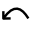
\includegraphics[width=0.7cm]{mActionUndo}
   & Défaire 
   & 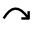
\includegraphics[width=0.7cm]{mActionRedo}
   & Refaire \\
\hline 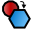
\includegraphics[width=0.7cm]{mActionSimplify}
   & Simplifier Entité
   & 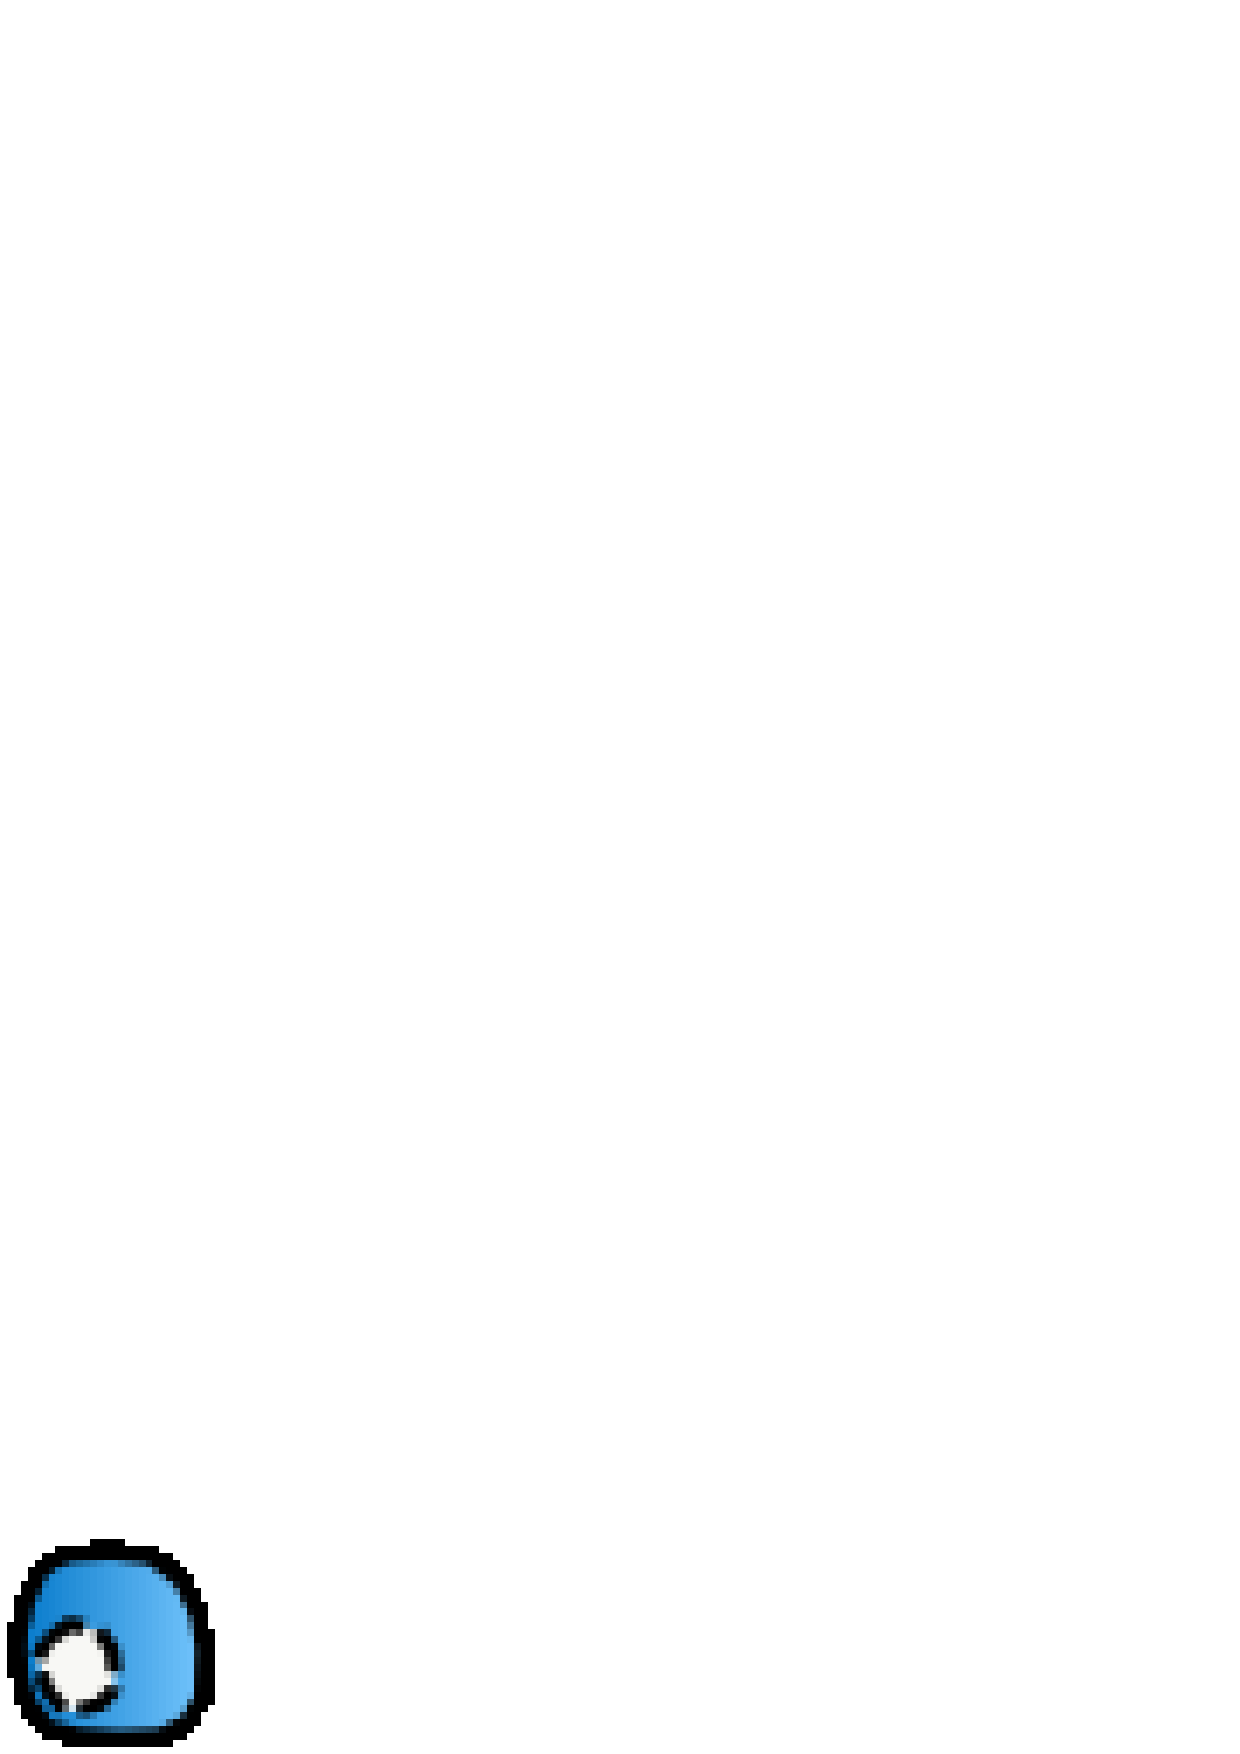
\includegraphics[width=0.7cm]{mActionAddRing}
   & Ajouter un anneau \\
\hline 
\includegraphics[width=0.7cm]{mActionAddIsland}
   & Ajouter une île
   & 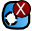
\includegraphics[width=0.7cm]{mActionDeleteRing}
   & Effacer un anneau \\
\hline 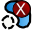
\includegraphics[width=0.7cm]{mActionDeletePart}
   & Effacer une partie
   & 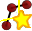
\includegraphics[width=0.7cm]{mActionReshape}
   & Remodeler une entité \\
\hline 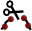
\includegraphics[width=0.7cm]{mActionSplitFeatures}
   & Couper une entité
   & 
\includegraphics[width=0.7cm]{mActionMergeFeatures}
   & Fusionner les entités sélectionnées \\
\hline 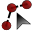
\includegraphics[width=0.7cm]{mActionNodeTool}
   & Outil de noeuds
   &
   & \\
\hline
\end{tabular}
\caption{Outils de numérisation avancée}\label{tab:advanced_editing}
\end{table}

\minisec{Annuler et refaire}
\index{couches vecteurs!annuler}
\index{couches vecteurs!refaire}

Les outils \toolbtntwo{mActionUndo}{Annuler} et \toolbtntwo{mActionRedo}{Refaire} permettent à l'utilisateur d'annuler ou revenir sur un certain nombre d'opérations sur les données vecteurs. La vue de base est une fenêtre où toutes les opérations sont répertoriées (voir figure~\ref{fig:vector_redoundo}). Cette fenêtre n'est pas affichée par défaut, mais peut être affichée par un clic droit sur une barre d'outils puis en cochant Annuler/Refaire L'outil est actif même quand la fenêtre n'est pas active.
\par
Quand on clique sur Annuler, l'état de toutes les entités retourne à l'état connu avant que les changements du à une opération quelconque aient été appliqué.
\par
Une action peut être déclenchée en cliquant sur les boutons Annuler ou Refaire (dans la fenêtre ou sur la barre d'outils de numérisation avancée) ou en cliquant directement sur l'action sur laquelle vous voulez revenir.

\begin{figure}[ht]
   \begin{center}   
   \includegraphics[clip=true, width=12cm]{redo_undo}
   \caption{Annuler et Refaire \nixcaption}\label{fig:vector_redoundo}
\end{center}
\end{figure}

% \minisec{Simplify Feature}
% \index{vector layers!simplify}
\minisec{Simplifier une entité}
\index{couches vecteurss!simplifier}

% The \toolbtntwo{mActionSimplify}{Simplify Feature} tool allows to reduce the
% number of vertices of a feature, as long as the geometry doesn't change. You 
% need to select one or several features, they will be highlighted by a red 
% rubber band and a slider appears. Moving the slider, the red rubber band is 
% changing its shape to show how the feature is being simplified. Clicking \button{OK} the new, simplified geometry will be stored. If a feature cannot be 
% simplified, a message shows up.
L'outil \toolbtntwo{mActionSimplify}{Simplifier une entité} permet de réduire le nombre de sommets qui composent une entité aussi longtemps que cela ne change pas le type de géométrie. Vous devez sélectionner une ou plusieurs entités qui seront alors sur-lignées par un contour rouge, une barre coulissante est affichée pour choisir le degré de simplification que vous désirez appliquer (le contour rouge reflète la forme que vous obtiendrez). Cliquez sur \button{OK} et la nouvelle forme sera retenue. Si une entité ne peut être simplifiée, un message vous le signalera.

% \minisec{Add Ring}
% \index{vector layers!add!ring}
\minisec{Ajouter un anneau}
\index{couches vecteurs!ajouter!anneau}

% You can create ring polygons using the \toolbtntwo{mActionAddRing}{Add Ring}
% icon in the toolbar. This means inside an existing area it is
% possible to digitize further polygons, that will occur as a 'hole', so only
% the area in between the boundaries of the outer and inner polygons remain as
% a ring polygon.

Vous pouvez créer des anneaux de polygones en utilisant l'icône \toolbtntwo{mActionAddRing}{Ajouter un anneau} Cela signifie qu'il est possible de dessiner des polygones à l'intérieur d'une zone existante et d'en tirer un trou,  seule la zone entre les limites externes des polygones sera conservée.

% \minisec{Add Island}
% \index{vector layers!add!island}
\minisec{Ajouter une île}
\index{couches vecteurs!ajouter!île}

% You can \toolbtntwo{mActionAddIsland}{add island} polygons to a selected
% multipolygon. The new island polygon has to be digitized outside the selected
% multipolygon.
Vous pouvez \toolbtntwo{mActionAddIsland}{ajouter une île} à un multipolygone sélectionné. La nouvelle île doit être dessinée en dehors de celui-ci.

% \minisec{Delete Ring}
% \index{vector layers!delete!ring}
\minisec{Effacer un anneau}
\index{couches vecteurs!effacer!anneau}

% The \toolbtntwo{mActionDeleteRing}{Delete Ring} tool allows to delete ring
% polygons inside an existing area. This tool only works with polygon layers. 
% It doesn't change anything when it is used on the outer ring of the polygon. 
% This tool can be used on polygon and mutli-polygon features.
L'outil \toolbtntwo{mActionDeleteRing}{Effacer un anneau} permet de supprimer un anneau existant. Il ne change rien lorsqu’utilisé sur la bordure extérieure du polygone.

% \minisec{Delete Part}
% \index{vector layers!delete!part}
\minisec{Effacer une partie}
\index{couches vecteurs!effacer!partie}

% The \toolbtntwo{mActionDeletePart}{Delete Part} tool allows to delete parts
% from multifeatures (e.g. to delete polygons from a multipolygon feature). It 
% won't delete the last part of the feature, this last part will stay untouched. This tool works with all multi-part geometries point, line and polygon.
L'outil \toolbtntwo{mActionDeletePart}{Effacer une partie} permet de supprimer des parties d'une entité multiparties (p.ex. un polygone composé de plusieurs polygones distincts). Cela n'effacera pas la dernière partie restante. Cet outil marche avec toutes les géométries.

% \minisec{Reshape Features}
% \index{vector layers!reshape!feature}
\minisec{Remodeler une entité}
\index{couches vecteurs!remodeler!entité}

% You can reshape line and polygon features using the 
% \toolbtntwo{mActionReshape}{Reshape Features} icon on the toolbar. It
% replaces the line or polygon part from the first to the last intersection 
% with the original line. With polygons this can sometime lead to unintended 
% results. It is mainly useful to replace smaller parts of a polygon, not major 
% overhauls and the reshapeline is not allowed to cross several polygon rings
% as this would generate an invalide polygon.
Il est possible de retoucher des lignes ou des polygones grâce à l'outil\\ \toolbtntwo{mActionReshape}{Remodeler une entité}. Vous pouvez changer la forme d'une ligne ou d'un polygone en traçant une nouvelle forme entre 2 sommets, la modification viendra s'ajouter à l'existant ou le remplacer selon la taille de l'intervalle entre le premier sommet et celui clôturant le remodelage. Cette méthode convient pour remplacer de petites portions d'une entité, la ligne de remodelage n'est pas autorisée à croiser plusieurs anneaux de polygones, car cela générerait un polygone invalide.

% \textbf{Note}: The reshape tool may alter the starting position of a polygon
% ring or a closed line. So the point that is represented 'twice' will not be
% the same any more. This may not be a problem for most applications, but it is
% something to consider.
\textbf{Note}: L'outil de remodelage peutt altérer la position de départ d'un anneau polygonal ou d'une ligne close, le point "double" ne sera plus le même. Ce n'est pas un problème pour la plupart des applications, mais c'est quelque chose à considérer.

% \minisec{Split Features}
% \index{vector layers!split!feature}
\minisec{Couper une entité}
\index{couches vecteurs!couper!entité}

% You can split features using the \toolbtntwo{mActionSplitFeatures}{Split
% Features} icon on the toolbar
Vous pouvez diviser une entité en utilisant le bouton \toolbtntwo{mActionSplitFeatures}{Couper Entités} situés dans la barre de numérisation.

% \minisec{Merge selected features}
% \index{vector layers!merge!features}
\minisec{Fusionner les entités sélectionnées}
\index{couches vecteurs!fusionner!entité}

% The \toolbtntwo{mActionMergeFeatures}{Merge Selected Features} tool allows to
% merge features that have common boundaries and the same attributes.  
L'outil \toolbtntwo{mActionMergeFeatures}{Fusionner les entités sélectionnées} permet de combiner des entités ayant une bordure commune et des attributs similaires.

% \minisec{Node Tool}
% \index{vector layers!node!tool}
\minisec{Outil de Noeuds}
\index{couches vecteurs!noeud!outil}

% The \toolbtntwo{mActionNodeTool}{Node Tool} provides manipulation capabilites
% of feature vertices similar to CAD programs. It is possible to simply select
% multiple vertices at once and to move, add or delete them alltogether. The node
% tool also works with 'on the fly' projection turned on and supports
% the topological editing feature. This tool is, unlike other tools in Quantum GIS, 
% persistent, so when some operation is done, selection stays active for this 
% feature and tool.

Le bouton \toolbtntwo{mActionNodeTool}{Outil de Noeuds} fournit la possibilité de manipuler des sommets d'entité de manière semblable à des programmes de CAO, on peut sélectionner facilement de multiples sommets à la fois et les déplacer, les effacer, les ajouter, etc. Cet outil fonctionne avec la projection "à la volée" activée et supporte l'édition topologique. Cet outil, au contraire des autres outils de \qg, est permanent donc quand une opération est effectuée, la sélection reste active pour cette entité et l'outil.

% \minisec{Basic operations}\index{vector layers!Node Tool}
\minisec{Opérations de base}\index{couches vecteurs!outil!noeud}

% Start by activating the \toolbtntwo{mActionNodeTool}{Node Tool} and selecting 
% some features by clicking on it. Red boxes appear at each vertex of this feature. 
% This is basic select of the feature. Functionalities are:
Commencez par activer l'outil \toolbtntwo{mActionNodeTool}{Outil de Noeuds} puis sélectionnez plusieurs entités en leur cliquant dessus. Un carré rouge apparaît sur chacun des sommets de ces entités. Les fonctionnalités sont :

\begin{description}
\item[Sélection d'un sommet :] elle se fait juste en cliquant sur le sommet, la couleur du carré virera au bleu. Lorsque vous voulez sélectionner plusieurs sommets, maintenez la touche \keystroke{Shift}. La touche \keystroke{Ctrl}  permet d'inverser la sélection (de les désélectionner si ils l'étaient). Plusieurs sommets peuvent être capturé en une fois en cliquant en dehors de la structure et en traçant un rectangle au-dessus d'eux. Ou encore, vous pouvez cliquez sur un segment et les sommets adjacents seront sélectionnés.
\item[Ajout d'un sommet :] Double-cliquez prêt d'un segment et un nouveau sommet apparaîtra proche du curseur. Veuillez noter que ce sommet apparaîtra sur le segment et non pas à la position du curseur, vous devrez donc le bouger si nécessaire.
\item[Effacer un sommet :] Après avoir fait vôtres sélection, utiliser la touche \keystroke{Supprimer} de votre clavier. Comme à son habitude \qg laissera assez de sommets pour garantir la conformité géométrique de l'entité, pour l'effacer complètement c'est un autre outil qu'il faudra employer.
\item[Déplacer un sommet :] Sélectionner tous les sommets que vous voulez, ils bougeront dans la même direction que le curseur. Si l'accrochage est activé, la sélection toute entière peut sauter jusqu'au sommet ou à la ligne la plus proche.
\end{description}

%\subsection{Creating a New Layer}\label{sec:create shape}\index{editing!creating a new layer}
\subsection{Créer une nouvelle couche}\label{sec:create shape}\index{éditer!créer une nouvelle couche}

%To create a new layer for editing, choose \toolbtntwo{mActionNewVectorLayer}{New Vector Layer} from the \mainmenuopt{Layer} menu. The \dialog{New Vector Layer} dialog will be displayed as shown in Figure \ref{fig:newvectorlayer}. Choose the type of layer (point, line or polygon).
Pour créer une nouvelle couche à éditer, allez dans \toolbtntwo{mActionNewVectorLayer}{Nouvelle couche vectorielle} du menu \mainmenuopt{Couche}. La fenêtre \dialog{Nouvelle couche vecteur} apparaitra telle que montrée dans la figure \ref{fig:newvectorlayer}. Choisissez le type de couche (point, ligne ou polygone).

\begin{figure}[ht]
  \begin{center}
  %\caption{Creating a New Vector Dialog \nixcaption}\label{fig:newvectorlayer}\smallskip
  \includegraphics[clip=true, width=8cm]{editNewVector}
  \caption{Fenêtre Nouvelle couche vecteur \nixcaption}\label{fig:newvectorlayer}
\end{center}
\end{figure}

%Note that \qg does not yet support creation of 2.5D features (i.e. features with X,Y,Z coordinates) or measure features. At this time, only shapefiles can be created. In a future version of \qg, creation of any OGR or \psq layer type will be supported.
Notez que \qg ne gère pas encore la création d'entité 2.5D (c.-à-d. des entités avec des coordonnées X, Y, Z). Pour le moment, seuls des shapefiles peuvent être créés. Dans une version future de \qg, la création de n'importe format de couches géré par OGR ou \psq sera possible.

%Creation of GRASS-layers is supported within the GRASS-plugin. Please refer to section \ref{sec:creating_new_grass_vectors} for more information on creating GRASS vector layers.
La création de couches GRASS est gérée par l'intermédiaire de l'extension GRASS. Référez-vous à la section \ref{sec:creating_new_grass_vectors} pour plus d'informations sur ce sujet.

%To complete the creation of the new layer, add the desired attributes by
%clicking on the \button{Add} button and specifying a name and type for the
%attribute. Only \selectstring{Type}{real}, \selectstring{Type}{integer}, and
%\selectstring{Type}{string} attributes are supported. Additionally and
%according to the attribute type you can also define the width and precision
%of the new attribute column. Once you are happy with the attributes, click
%\button{OK} and provide a name for the shapefile. \qg will automatically add
%a \filename{.shp} extension to the name you specify. Once
%the layer has been created, it will be added to the map and you can edit it in
%the same way as described in Section \ref{sec:edit_existing_layer} above. 
Pour terminer la création de la nouvelle couche, ajouter les attributs désirés en cliquant sur le bouton \button{Ajouter un attribut} et en spécifiant le nom et le type de l'attribut. Seuls les attributs de type \selectstring{Type}{réel}, \selectstring{Type}{entier}, et \selectstring{Type}{string} sont gérés. De plus, selon le type d'attribut vous pouvez définir la largeur et la précision de la nouvelle colonne. Une fois satisfait de vos attributs, cliquez sur \button{OK} et donnez un nom pour le shapefile. \qg va automatiquement ajouter l'extension \filename{.shp} au nom que vous lui avez spécifié. Une fois la couche créée, elle sera ajoutée à la carte et vous pouvez l'éditer de la manière décrite dans la Section \ref{sec:edit_existing_layer} ci-dessus.

%\subsection{Working with the Attribute Table}\label{sec:attribute table}\index{editing!working with the attribute table}
\subsection{Travailler avec la table attributaire}\label{sec:attribute table}\index{éditer!travailler avec la table attributaire}

%The attribute table displays features of a selected layer. Each row in the table 
%represents one map feature with its attributes shown in several columns. The 
%features in the table can be searched, selected, moved or even edited.
La table attributaire affiche les entités de la couche sélectionnée. Chaque ligne représente une entité avec ses attributs répartis dans  plusieurs colonnes. Chaque entité de la table peut être recherchée, sélectionnée, déplacée et éditée.

%To open the attribute table for a vector layer, make the layer active by clicking 
%on it in the map legend area. Then use \mainmenuopt{Layer} from the main menu 
%and and choose \dropmenuopttwo{mActionOpenTable}{Open Attribute Table} 
%from the menu. It is also possible to rightlick on the layer and 
%choose \dropmenuopttwo{mActionOpenTable}{Open Attribute Table} from the 
%dropdown menu. This will open a new window which displays the attributes for 
%every feature in the layer (figure \ref{fig:attributetable}).
Pour ouvrir la table attributaire d'une couche vecteur, acitvez la couche en cliquant dessus depuis la zone de légende de la carte. Puis dans le menu  \mainmenuopt{Couche}, faites and and choose \dropmenuopttwo{mActionOpenTable}{Ouvrir la table d'attribut}. Vous pouvez aussi y accéder avec un clic droit sur la couche. Cela ouvrira une nouvelle fenêtre qui comportera les attributs de toutes les entités de la couche (voir figure \ref{fig:attributetable}).

\begin{figure}[ht]
   \begin{center}
   \includegraphics[clip=true, width=12cm]{vectorAttributeTable}
    \caption{Table d'attributs pour la couche Alaska \nixcaption}\label{fig:attributetable}
\end{center} 
\end{figure}

\minisec{Sélectionner une entité depuis la table}

%\textbf{A selected row} in the attribute table represents all attributes of a 
%selected feature in the layer. The attribute table reflects any changes 
%in the layer selection in the main window and vice versa. A changed selection 
%in the attribute table also causes a change in the selected feature set in the 
%main window and different layer feature selection means different rows are to be 
%selected.

\textbf{Une ligne sélectionnée} représente tout les attributs d'une entité, la table attributaire reflète tous les changements qui seront faits sur la carte et vice versa. Un changement de sélection depuis la table d'attributs provoque également un changement de sélection sur la carte et la sélection d'entités d'une couche différente signifie que d'autres lignes ont été sélectionnées.

%Rows can be selected by clicking on the row number on the left side of the 
%row. Selecting a row doesn't change the current cursor position. \textbf{Multiple 
%rows} can be marked by holding the \keystroke{Ctrl} key. A \textbf{continuous 
%selection} can be made by holding the \keystroke{Shift} key and clicking on several 
%row headers on the left side of the rows. All rows between the current cursor 
%position and the clicked row are selected.

Les lignes peuvent être sélectionnées en cliquant sur le numéro de ligne placé tout à gauche. La sélection d'une ligne ne cause pas de changement de position du curseur. \textbf{Plusieurs lignes} peuvent être retenues en maintenant la touche \textbf{Ctrl}. \textbf{Une sélection continue} s'effectue en gardant appuyé la touche \textbf{Shift} et en cliquant sur une nouvelle ligne, toutes les lignes entrera première sélection et la dernière seront prises.

%Each column can be sorted by clicking on its column header. A small arrow 
%indicates the sort order (downward pointing means descending values from the top 
%row down, upward pointing means ascending values from the top rown down).
Vous pouvez faire un tri sur les colonnes en cliquant sur l'en-tête. Une petite flèche indique l'ordre de tri (une flèche pointant vers le bas indiquera un tri descendant).

%For a \textbf{simple search by attributes} on only one column the \button{Look for} 
%field can be used. Select the field (column) from which the search should be 
%performed from the dropdown menu and hit the \button{Search} button. For more 
%complex searches use the Advanced search \button{...}, which will lauch the 
%Search Query Builder described in Section \ref{sec:select_by_query}. 
Pour une \textbf{simple recherche par attributs} sur une colonne seulement, il faut utiliser le champ de saisie \button{Chercher pour}. Choisissez la colonne sur laquelle doit s'opérer la recherche depuis le menu déroulant de droite et appuyez sur le bouton \button{Chercher}. Pour des recherches plus complexes, il vous faudra cliquer sur \button{Recherche avancée} qui ouvrira le constructeur de requête décrit dans la section \ref{sec:select_by_query}.

%To show selected records only, use the checkbox \checkbox{Show selected records only}. To search selected records only, use the checkbox \checkbox{Search selected records only}. The other buttons at the bottom left of the attribute table window provide following functionality: 
Pour afficher uniquement les enregistrements que vous avez sélectionnés, utiliser la boite à cocher \checkbox{Montrer seulement les enregistrements sélectionnés}. Pour limiter la recherche à la sélection, activer la boîte à cocher \checkbox{Rechercher seulement les enregistrements sélectionnés} Les autres boutons disposés à gauche de la fenêtre fournissent les fonctionnalités suivantes :

%\begin{itemize}
%\item \toolbtntwo{mActionOpenTable}{Remove selection}
%\item \toolbtntwo{mActionSelectedToTop}{Move selected to top}
%\item \toolbtntwo{mActionInvertSelection}{Invert selection}
%\item \toolbtntwo{mActionCopySelected}{Copy selected rows to clipboard} also with \keystroke{Ctrl-C}
%\item \toolbtntwo{mActionZoomToSelected}{Zoom map to selected rows} also with \keystroke{Ctrl-J}
%\item \toolbtntwo{mActionToggleEditing}{toggle editing mode} to edit single values of attribute table.
%\end{itemize}
\begin{itemize}[label=--]
\item \toolbtntwo{mActionOpenTable}{Desélectionner tout}
\item \toolbtntwo{mActionSelectedToTop}{Déplacer la sélection au sommet}
\item \toolbtntwo{mActionInvertSelection}{Inverser la sélection}
\item \toolbtntwo{mActionCopySelected}{Copier les lignes sélectionnées dans le presse-papier} ou \keystroke{Ctrl-C}
\item \toolbtntwo{mActionZoomToSelected}{Zoomer la carte sur les lignes sélectionnées} ou \keystroke{Ctrl-J}
\item \toolbtntwo{mActionToggleEditing}{Activer le mode d'édition} pour modifier les valeurs des attributs
\end{itemize}

%\begin{Tip}[ht]\caption{\textsc{Manipulating Attribute data}}
%\qgistip{Currently only \pg layers are supported for adding or dropping
%attribute columns within this dialog. In future versions of \qg, other
%datasources will be supported, because this feature was recently implemented
%in GDAL/OGR > 1.6.0
\begin{Tip}[ht]\caption{\textsc{Manipuler les données attributaires}}
Actuellement seules les couches \pg sont supportés pour ce quide l'ajout ou la suppression de colonnes. Les prochaines versions de \qg étendront ce support à d'autres sources de données grâce aux apports des versions de GDAL/OGR postérieures à la 1.6.0.
\end{Tip}

%\section{Query Builder}\label{sec:query_builder}
\section{Constructeur de requêtes}\label{sec:query_builder}
%\index{Query Builder}
\index{Constructeur de requêtes}

%The \button{Advanced search\dots} button opens the Query Builder and allows you to define a subset of a table using a SQL-like WHERE clause, display the result in the main window and save it as a Shapefile. For example, if you have a \filename{towns} layer %with a \usertext{population} field you could select only larger towns by entering \usertext{population > 100000} in the SQL box of the query builder. Figure
%\ref{fig:query_builder} shows an example of the query builder populated with
%data from a \pg layer with attributes stored in PostgreSQL. 
%The Fields, Values and Operators sections help the user to construct the SQL-like

Le bouton de recherche avancée ouvre le constructeur de requêtes qui vous permet de définir un sous-ensemble de la table en utilisant une clause SQL de type WHERE et de l'afficher comme une couche dans \qg. Par exemple, si vous avez une couche \filename{towns} avec un champ \usertext{population}, vous pouvez sélectionner uniquement les plus grandes villes en entrant \usertext{population >\,\numprint{100000}} dans le cadre SQL du constructeur de requête. La figure \ref{fig:query_builder} montre un exemple de requête avec les données d'une couche \pg dont les attributs sont stockés dans PostgreSQL.

\begin{figure}[ht]
  \begin{center}
    %\caption{Query Builder \nixcaption}\label{fig:query_builder}\smallskip
    \includegraphics[clip=true, width=11.5cm]{queryBuilder}
    \caption{Constructeur de requêtes \nixcaption} \label{fig:query_builder}
  \end{center}
\end{figure}

%The \textbf{Fields list} contains all attributes of the attribute table to be 
%searched. To add an attribute to the SQL where clause field, double click its 
%name in the Fields list. Generally you can use the various fields, values and 
%operators to construct the query or you can just type it into the SQL box. 
La liste des champs contient tous les attributs de la table attributaire pouvant être parcourus par la recherche. Pour ajouter un attribut à la clause WHERE, double-cliquez son nom dans cette liste. Vous pouvez cliquez sur les différents champs, valeurs et opérateurs qui composent votre requête ou bien l'écrire directement dans le cadre SQL.

%The \textbf{Values list} lists the values of an attribute. To list all possible 
%values of an attribute, select the attribute in the Fields list and click the 
%\button{All} button\index{Query Builder!getting all values}. To list all values 
%of an attribute that are present in the sample table, select the attribute in 
%the Fields list and click the \button{Sample} button\index{Query Builder!generating sample list}. To add a value to the SQL 
%where clause field, double click its name in the Values list.   
La liste des valeurs recense toutes les valeurs d'un attribut. Pour en lister la totalité, sélectionnez l'attribut dans la liste de champs puis cliquez sur le bouton \button{Tout}\index{constructeur de requête!obtenir toutes les valeurs}. Pour lister toutes les valeurs présentes dans la liste d'échantillons, sélectionnez l'attribut puis le bouton \button{Echantillon}\index{constructeur de requête!générer une liste d'échantillon}. Pour ajouter une valeur à la clause WHERE et la prendre en compte dans la requête, il vous suffit de faire un double-clic dessus.

%The \textbf{Operators section} contains all usable operators. To add an operator 
%to the SQL where clause field, click the appropriate button. Relational operators 
%( = , > , \dots), string comparison operator ( LIKE ), logical operators ( AND , OR 
%, \dots) are available. 
La section des opérateurs contient toutes les opérations menables sur une recherche. Pour ajouter un opérateur à la requête SQL, cliquez sur le bouton approprié. Les opérateurs relationnels (=, >, \dots), les opérateurs de comparaison (LIKE), les opérateurs logiques ( AND, OR,\dots) sont disponibles.

%The \button{Clear} button clears the text in the SQL where clause text field. The 
%\button{Test} button shows a message box with the number of features satisfying 
%the current query, which is usable in the process of query construction. The 
%\button{OK} button closes the window and selects the features satisfying the 
%query. The \button{Cancel} button closes the window without changing the current 
%selection. 
Le bouton \button{Effacer} nettoye le texte présent dans le cadre SQL.button clears the text in the SQL where clause text field. Le \button{Test} affiche une fenêtre comptabilisant le nombre d'entités satisfaisant à votre requête, vous permettant de savoir si votre requête fonctionne au fil de sa construction. Le bouton \button{OK} ferme la fenêtre et effectue la recherche définie. Le bouton \button{Annuler} clôt la fenêtre, mais sans la sélection en cours.

%\begin{Tip}\caption{\textsc{Changing the Layer Definition}}\index{Query Builder!changing layer definitions}
\begin{Tip}\caption{\textsc{Changer la définition d'une couche}}\index{Constructeur de requête!changer des définitions de couche}
%\qgistip{You can change the layer definition after it is loaded by altering the SQL query used to define the layer. To do this, open the  vector \dialog{Layer Properties} dialog by double-clicking on the layer in the legend and click on the \button{Query Builder} button on the \tab{General} tab. See Section \ref{sec:vectorprops} for more information.}
Vous pouvez changer la définition d'une couche après son chargement en modifiant la requête SQL utilisée pour définir la couche. Pour faire cela, ouvrez la fenêtre \dialog{Propriétés de la couche} en double-cliquant sur la couche dans la légende puis cliquez sur le bouton \button{Constructeur de requête} dans l'onglet \tab{Général}. Voir Section \ref{sec:vectorprops} pour plus d'informations.
\end{Tip}

%\section{Select by query}\label{sec:select_by_query}
%\index{PostgreSQL!query builder}
%\index{PostGIS!query builder}
%\index{query builder!PostgreSQL}
%\index{query builder!PostGIS}
\section{Sélection par requête}\label{sec:select_by_query}
\index{PostgreSQL!constructeur de requête}
\index{PostGIS!constructeur de requête}
\index{constructeur de requête!PostgreSQL}
\index{constructeur de requête!PostGIS}

%With \qg it is possible also to select features using a similar query builder interface to that used in \ref{sec:query_builder}. In the above section the purpose of the query builder is to only show features meeting the filter criteria as a 'virtual layer' / subset. The purpose of the select by query function is to highlight all features that meet a particular criteria. Select by query can be used with all vector data providers.
Dans \qg, il est possible de sélectionner des entités en utilisant une interface similaire à celle du constructeur de requêtes utilisé dans \ref{sec:query_builder}. Dans la section ci-dessus, le but du constructeur de requêtes était seulement de montrer les entités répondant aux critères de filtre comme une \og couche virtuelle\fg/ sous-ensemble. Le but de la fonction de sélection par requête est de surligner toutes les entités qui répondent à un critère particulier. La sélection par requête peut être utilisée sur tous les fournisseurs de données vecteur.

%To do a `select by query' on a loaded layer, click on the button \toolbtntwo{mActionOpenTable}{Open Table} to open the attribute table of the layer. Then click the \button{Advanced...} button at the bottom. This starts the Query Builder that allows to define a subset of a table and display it as described in Section \ref{sec:query_builder}.
Pour faire une \og sélection par requête\fg sur une couche chargée, cliquez sur le bouton\\ \toolbtntwo{mActionOpenTable}{Ouvrir la table des attributs} pour ouvrir la table de la couche. Ensuite cliquez sur le bouton \button{Avancée\dots} en bas de la fenêtre. Cela lance le Constructeur de requête qui permet de définir un sous-ensemble de la table et l'affiche comme décrit dans la Section \ref{sec:query_builder}.


%\index{vector layers|)}
\index{couches vecteur|)}

